\documentclass[11pt]{article}

    \usepackage[spanish]{babel}
    \usepackage{parskip} % Stop auto-indenting (to mimic markdown behaviour)
    

    % Basic figure setup, for now with no caption control since it's done
    % automatically by Pandoc (which extracts ![](path) syntax from Markdown).
    \usepackage{graphicx}
    % Maintain compatibility with old templates. Remove in nbconvert 6.0
    \let\Oldincludegraphics\includegraphics
    % Ensure that by default, figures have no caption (until we provide a
    % proper Figure object with a Caption API and a way to capture that
    % in the conversion process - todo).
    \usepackage{caption}
    \DeclareCaptionFormat{nocaption}{}
    \captionsetup{format=nocaption,aboveskip=0pt,belowskip=0pt}

    \usepackage{float}
    \floatplacement{figure}{H} % forces figures to be placed at the correct location
    \usepackage{xcolor} % Allow colors to be defined
    \usepackage{enumerate} % Needed for markdown enumerations to work
    \usepackage{geometry} % Used to adjust the document margins
    \usepackage{amsmath} % Equations
    \usepackage{amssymb} % Equations
    \usepackage{textcomp} % defines textquotesingle
    % Hack from http://tex.stackexchange.com/a/47451/13684:
    \AtBeginDocument{%
        \def\PYZsq{\textquotesingle}% Upright quotes in Pygmentized code
    }
    \usepackage{upquote} % Upright quotes for verbatim code
    \usepackage{eurosym} % defines \euro

    \usepackage{iftex}
    \ifPDFTeX
        \usepackage[T1]{fontenc}
        \IfFileExists{alphabeta.sty}{
              \usepackage{alphabeta}
          }{
              \usepackage[mathletters]{ucs}
              \usepackage[utf8x]{inputenc}
          }
    \else
        \usepackage{fontspec}
        \usepackage{unicode-math}
    \fi

    \usepackage{fancyvrb} % verbatim replacement that allows latex
    \usepackage{grffile} % extends the file name processing of package graphics
                         % to support a larger range
    \makeatletter % fix for old versions of grffile with XeLaTeX
    \@ifpackagelater{grffile}{2019/11/01}
    {
      % Do nothing on new versions
    }
    {
      \def\Gread@@xetex#1{%
        \IfFileExists{"\Gin@base".bb}%
        {\Gread@eps{\Gin@base.bb}}%
        {\Gread@@xetex@aux#1}%
      }
    }
    \makeatother
    \usepackage[Export]{adjustbox} % Used to constrain images to a maximum size
    \adjustboxset{max size={0.9\linewidth}{0.9\paperheight}}

    % The hyperref package gives us a pdf with properly built
    % internal navigation ('pdf bookmarks' for the table of contents,
    % internal cross-reference links, web links for URLs, etc.)
    \usepackage{hyperref}
    % The default LaTeX title has an obnoxious amount of whitespace. By default,
    % titling removes some of it. It also provides customization options.
    \usepackage{titling}
    \usepackage{longtable} % longtable support required by pandoc >1.10
    \usepackage{booktabs}  % table support for pandoc > 1.12.2
    \usepackage{array}     % table support for pandoc >= 2.11.3
    \usepackage{calc}      % table minipage width calculation for pandoc >= 2.11.1
    \usepackage[inline]{enumitem} % IRkernel/repr support (it uses the enumerate* environment)
    \usepackage[normalem]{ulem} % ulem is needed to support strikethroughs (\sout)
                                % normalem makes italics be italics, not underlines
    \usepackage{soul}      % strikethrough (\st) support for pandoc >= 3.0.0
    \usepackage{mathrsfs}
    \usepackage{capt-of}
    \usepackage{adjustbox}
    \usepackage[T1]{fontenc}
    \usepackage[most]{tcolorbox}
    \usepackage{lmodern} 
    

    
    % Colors for the hyperref package
    \definecolor{urlcolor}{rgb}{0,.145,.698}
    \definecolor{linkcolor}{rgb}{.71,0.21,0.01}
    \definecolor{citecolor}{rgb}{.12,.54,.11}

    % ANSI colors
    \definecolor{ansi-black}{HTML}{3E424D}
    \definecolor{ansi-black-intense}{HTML}{282C36}
    \definecolor{ansi-red}{HTML}{E75C58}
    \definecolor{ansi-red-intense}{HTML}{B22B31}
    \definecolor{ansi-green}{HTML}{00A250}
    \definecolor{ansi-green-intense}{HTML}{007427}
    \definecolor{ansi-yellow}{HTML}{DDB62B}
    \definecolor{ansi-yellow-intense}{HTML}{B27D12}
    \definecolor{ansi-blue}{HTML}{208FFB}
    \definecolor{ansi-blue-intense}{HTML}{0065CA}
    \definecolor{ansi-magenta}{HTML}{D160C4}
    \definecolor{ansi-magenta-intense}{HTML}{A03196}
    \definecolor{ansi-cyan}{HTML}{60C6C8}
    \definecolor{ansi-cyan-intense}{HTML}{258F8F}
    \definecolor{ansi-white}{HTML}{C5C1B4}
    \definecolor{ansi-white-intense}{HTML}{A1A6B2}
    \definecolor{ansi-default-inverse-fg}{HTML}{FFFFFF}
    \definecolor{ansi-default-inverse-bg}{HTML}{000000}

    % common color for the border for error outputs.
    \definecolor{outerrorbackground}{HTML}{FFDFDF}

    % commands and environments needed by pandoc snippets
    % extracted from the output of `pandoc -s`
    \providecommand{\tightlist}{%
      \setlength{\itemsep}{0pt}\setlength{\parskip}{0pt}}
    \DefineVerbatimEnvironment{Highlighting}{Verbatim}{commandchars=\\\{\}}
    % Add ',fontsize=\small' for more characters per line
    \newenvironment{Shaded}{}{}
    \newcommand{\KeywordTok}[1]{\textcolor[rgb]{0.00,0.44,0.13}{\textbf{{#1}}}}
    \newcommand{\DataTypeTok}[1]{\textcolor[rgb]{0.56,0.13,0.00}{{#1}}}
    \newcommand{\DecValTok}[1]{\textcolor[rgb]{0.25,0.63,0.44}{{#1}}}
    \newcommand{\BaseNTok}[1]{\textcolor[rgb]{0.25,0.63,0.44}{{#1}}}
    \newcommand{\FloatTok}[1]{\textcolor[rgb]{0.25,0.63,0.44}{{#1}}}
    \newcommand{\CharTok}[1]{\textcolor[rgb]{0.25,0.44,0.63}{{#1}}}
    \newcommand{\StringTok}[1]{\textcolor[rgb]{0.25,0.44,0.63}{{#1}}}
    \newcommand{\CommentTok}[1]{\textcolor[rgb]{0.38,0.63,0.69}{\textit{{#1}}}}
    \newcommand{\OtherTok}[1]{\textcolor[rgb]{0.00,0.44,0.13}{{#1}}}
    \newcommand{\AlertTok}[1]{\textcolor[rgb]{1.00,0.00,0.00}{\textbf{{#1}}}}
    \newcommand{\FunctionTok}[1]{\textcolor[rgb]{0.02,0.16,0.49}{{#1}}}
    \newcommand{\RegionMarkerTok}[1]{{#1}}
    \newcommand{\ErrorTok}[1]{\textcolor[rgb]{1.00,0.00,0.00}{\textbf{{#1}}}}
    \newcommand{\NormalTok}[1]{{#1}}

    % Additional commands for more recent versions of Pandoc
    \newcommand{\ConstantTok}[1]{\textcolor[rgb]{0.53,0.00,0.00}{{#1}}}
    \newcommand{\SpecialCharTok}[1]{\textcolor[rgb]{0.25,0.44,0.63}{{#1}}}
    \newcommand{\VerbatimStringTok}[1]{\textcolor[rgb]{0.25,0.44,0.63}{{#1}}}
    \newcommand{\SpecialStringTok}[1]{\textcolor[rgb]{0.73,0.40,0.53}{{#1}}}
    \newcommand{\ImportTok}[1]{{#1}}
    \newcommand{\DocumentationTok}[1]{\textcolor[rgb]{0.73,0.13,0.13}{\textit{{#1}}}}
    \newcommand{\AnnotationTok}[1]{\textcolor[rgb]{0.38,0.63,0.69}{\textbf{\textit{{#1}}}}}
    \newcommand{\CommentVarTok}[1]{\textcolor[rgb]{0.38,0.63,0.69}{\textbf{\textit{{#1}}}}}
    \newcommand{\VariableTok}[1]{\textcolor[rgb]{0.10,0.09,0.49}{{#1}}}
    \newcommand{\ControlFlowTok}[1]{\textcolor[rgb]{0.00,0.44,0.13}{\textbf{{#1}}}}
    \newcommand{\OperatorTok}[1]{\textcolor[rgb]{0.40,0.40,0.40}{{#1}}}
    \newcommand{\BuiltInTok}[1]{{#1}}
    \newcommand{\ExtensionTok}[1]{{#1}}
    \newcommand{\PreprocessorTok}[1]{\textcolor[rgb]{0.74,0.48,0.00}{{#1}}}
    \newcommand{\AttributeTok}[1]{\textcolor[rgb]{0.49,0.56,0.16}{{#1}}}
    \newcommand{\InformationTok}[1]{\textcolor[rgb]{0.38,0.63,0.69}{\textbf{\textit{{#1}}}}}
    \newcommand{\WarningTok}[1]{\textcolor[rgb]{0.38,0.63,0.69}{\textbf{\textit{{#1}}}}}


    % Define a nice break command that doesn't care if a line doesn't already
    % exist.
    \def\br{\hspace*{\fill} \\* }
    % Math Jax compatibility definitions
    \def\gt{>}
    \def\lt{<}
    \let\Oldtex\TeX
    \let\Oldlatex\LaTeX
    \renewcommand{\TeX}{\textrm{\Oldtex}}
    \renewcommand{\LaTeX}{\textrm{\Oldlatex}}
    % Document parameters
    % Document title
    \title{Laboratorio: Modelos del lenguaje con RNNs}
    \author{Néstor Batista Díaz}
    \date{}
    
    
    
    
    
    
    
    
% Pygments definitions
\makeatletter
\def\PY@reset{\let\PY@it=\relax \let\PY@bf=\relax%
    \let\PY@ul=\relax \let\PY@tc=\relax%
    \let\PY@bc=\relax \let\PY@ff=\relax}
\def\PY@tok#1{\csname PY@tok@#1\endcsname}
\def\PY@toks#1+{\ifx\relax#1\empty\else%
    \PY@tok{#1}\expandafter\PY@toks\fi}
\def\PY@do#1{\PY@bc{\PY@tc{\PY@ul{%
    \PY@it{\PY@bf{\PY@ff{#1}}}}}}}
\def\PY#1#2{\PY@reset\PY@toks#1+\relax+\PY@do{#2}}

\@namedef{PY@tok@w}{\def\PY@tc##1{\textcolor[rgb]{0.73,0.73,0.73}{##1}}}
\@namedef{PY@tok@c}{\let\PY@it=\textit\def\PY@tc##1{\textcolor[rgb]{0.24,0.48,0.48}{##1}}}
\@namedef{PY@tok@cp}{\def\PY@tc##1{\textcolor[rgb]{0.61,0.40,0.00}{##1}}}
\@namedef{PY@tok@k}{\let\PY@bf=\textbf\def\PY@tc##1{\textcolor[rgb]{0.00,0.50,0.00}{##1}}}
\@namedef{PY@tok@kp}{\def\PY@tc##1{\textcolor[rgb]{0.00,0.50,0.00}{##1}}}
\@namedef{PY@tok@kt}{\def\PY@tc##1{\textcolor[rgb]{0.69,0.00,0.25}{##1}}}
\@namedef{PY@tok@o}{\def\PY@tc##1{\textcolor[rgb]{0.40,0.40,0.40}{##1}}}
\@namedef{PY@tok@ow}{\let\PY@bf=\textbf\def\PY@tc##1{\textcolor[rgb]{0.67,0.13,1.00}{##1}}}
\@namedef{PY@tok@nb}{\def\PY@tc##1{\textcolor[rgb]{0.00,0.50,0.00}{##1}}}
\@namedef{PY@tok@nf}{\def\PY@tc##1{\textcolor[rgb]{0.00,0.00,1.00}{##1}}}
\@namedef{PY@tok@nc}{\let\PY@bf=\textbf\def\PY@tc##1{\textcolor[rgb]{0.00,0.00,1.00}{##1}}}
\@namedef{PY@tok@nn}{\let\PY@bf=\textbf\def\PY@tc##1{\textcolor[rgb]{0.00,0.00,1.00}{##1}}}
\@namedef{PY@tok@ne}{\let\PY@bf=\textbf\def\PY@tc##1{\textcolor[rgb]{0.80,0.25,0.22}{##1}}}
\@namedef{PY@tok@nv}{\def\PY@tc##1{\textcolor[rgb]{0.10,0.09,0.49}{##1}}}
\@namedef{PY@tok@no}{\def\PY@tc##1{\textcolor[rgb]{0.53,0.00,0.00}{##1}}}
\@namedef{PY@tok@nl}{\def\PY@tc##1{\textcolor[rgb]{0.46,0.46,0.00}{##1}}}
\@namedef{PY@tok@ni}{\let\PY@bf=\textbf\def\PY@tc##1{\textcolor[rgb]{0.44,0.44,0.44}{##1}}}
\@namedef{PY@tok@na}{\def\PY@tc##1{\textcolor[rgb]{0.41,0.47,0.13}{##1}}}
\@namedef{PY@tok@nt}{\let\PY@bf=\textbf\def\PY@tc##1{\textcolor[rgb]{0.00,0.50,0.00}{##1}}}
\@namedef{PY@tok@nd}{\def\PY@tc##1{\textcolor[rgb]{0.67,0.13,1.00}{##1}}}
\@namedef{PY@tok@s}{\def\PY@tc##1{\textcolor[rgb]{0.73,0.13,0.13}{##1}}}
\@namedef{PY@tok@sd}{\let\PY@it=\textit\def\PY@tc##1{\textcolor[rgb]{0.73,0.13,0.13}{##1}}}
\@namedef{PY@tok@si}{\let\PY@bf=\textbf\def\PY@tc##1{\textcolor[rgb]{0.64,0.35,0.47}{##1}}}
\@namedef{PY@tok@se}{\let\PY@bf=\textbf\def\PY@tc##1{\textcolor[rgb]{0.67,0.36,0.12}{##1}}}
\@namedef{PY@tok@sr}{\def\PY@tc##1{\textcolor[rgb]{0.64,0.35,0.47}{##1}}}
\@namedef{PY@tok@ss}{\def\PY@tc##1{\textcolor[rgb]{0.10,0.09,0.49}{##1}}}
\@namedef{PY@tok@sx}{\def\PY@tc##1{\textcolor[rgb]{0.00,0.50,0.00}{##1}}}
\@namedef{PY@tok@m}{\def\PY@tc##1{\textcolor[rgb]{0.40,0.40,0.40}{##1}}}
\@namedef{PY@tok@gh}{\let\PY@bf=\textbf\def\PY@tc##1{\textcolor[rgb]{0.00,0.00,0.50}{##1}}}
\@namedef{PY@tok@gu}{\let\PY@bf=\textbf\def\PY@tc##1{\textcolor[rgb]{0.50,0.00,0.50}{##1}}}
\@namedef{PY@tok@gd}{\def\PY@tc##1{\textcolor[rgb]{0.63,0.00,0.00}{##1}}}
\@namedef{PY@tok@gi}{\def\PY@tc##1{\textcolor[rgb]{0.00,0.52,0.00}{##1}}}
\@namedef{PY@tok@gr}{\def\PY@tc##1{\textcolor[rgb]{0.89,0.00,0.00}{##1}}}
\@namedef{PY@tok@ge}{\let\PY@it=\textit}
\@namedef{PY@tok@gs}{\let\PY@bf=\textbf}
\@namedef{PY@tok@ges}{\let\PY@bf=\textbf\let\PY@it=\textit}
\@namedef{PY@tok@gp}{\let\PY@bf=\textbf\def\PY@tc##1{\textcolor[rgb]{0.00,0.00,0.50}{##1}}}
\@namedef{PY@tok@go}{\def\PY@tc##1{\textcolor[rgb]{0.44,0.44,0.44}{##1}}}
\@namedef{PY@tok@gt}{\def\PY@tc##1{\textcolor[rgb]{0.00,0.27,0.87}{##1}}}
\@namedef{PY@tok@err}{\def\PY@bc##1{{\setlength{\fboxsep}{\string -\fboxrule}\fcolorbox[rgb]{1.00,0.00,0.00}{1,1,1}{\strut ##1}}}}
\@namedef{PY@tok@kc}{\let\PY@bf=\textbf\def\PY@tc##1{\textcolor[rgb]{0.00,0.50,0.00}{##1}}}
\@namedef{PY@tok@kd}{\let\PY@bf=\textbf\def\PY@tc##1{\textcolor[rgb]{0.00,0.50,0.00}{##1}}}
\@namedef{PY@tok@kn}{\let\PY@bf=\textbf\def\PY@tc##1{\textcolor[rgb]{0.00,0.50,0.00}{##1}}}
\@namedef{PY@tok@kr}{\let\PY@bf=\textbf\def\PY@tc##1{\textcolor[rgb]{0.00,0.50,0.00}{##1}}}
\@namedef{PY@tok@bp}{\def\PY@tc##1{\textcolor[rgb]{0.00,0.50,0.00}{##1}}}
\@namedef{PY@tok@fm}{\def\PY@tc##1{\textcolor[rgb]{0.00,0.00,1.00}{##1}}}
\@namedef{PY@tok@vc}{\def\PY@tc##1{\textcolor[rgb]{0.10,0.09,0.49}{##1}}}
\@namedef{PY@tok@vg}{\def\PY@tc##1{\textcolor[rgb]{0.10,0.09,0.49}{##1}}}
\@namedef{PY@tok@vi}{\def\PY@tc##1{\textcolor[rgb]{0.10,0.09,0.49}{##1}}}
\@namedef{PY@tok@vm}{\def\PY@tc##1{\textcolor[rgb]{0.10,0.09,0.49}{##1}}}
\@namedef{PY@tok@sa}{\def\PY@tc##1{\textcolor[rgb]{0.73,0.13,0.13}{##1}}}
\@namedef{PY@tok@sb}{\def\PY@tc##1{\textcolor[rgb]{0.73,0.13,0.13}{##1}}}
\@namedef{PY@tok@sc}{\def\PY@tc##1{\textcolor[rgb]{0.73,0.13,0.13}{##1}}}
\@namedef{PY@tok@dl}{\def\PY@tc##1{\textcolor[rgb]{0.73,0.13,0.13}{##1}}}
\@namedef{PY@tok@s2}{\def\PY@tc##1{\textcolor[rgb]{0.73,0.13,0.13}{##1}}}
\@namedef{PY@tok@sh}{\def\PY@tc##1{\textcolor[rgb]{0.73,0.13,0.13}{##1}}}
\@namedef{PY@tok@s1}{\def\PY@tc##1{\textcolor[rgb]{0.73,0.13,0.13}{##1}}}
\@namedef{PY@tok@mb}{\def\PY@tc##1{\textcolor[rgb]{0.40,0.40,0.40}{##1}}}
\@namedef{PY@tok@mf}{\def\PY@tc##1{\textcolor[rgb]{0.40,0.40,0.40}{##1}}}
\@namedef{PY@tok@mh}{\def\PY@tc##1{\textcolor[rgb]{0.40,0.40,0.40}{##1}}}
\@namedef{PY@tok@mi}{\def\PY@tc##1{\textcolor[rgb]{0.40,0.40,0.40}{##1}}}
\@namedef{PY@tok@il}{\def\PY@tc##1{\textcolor[rgb]{0.40,0.40,0.40}{##1}}}
\@namedef{PY@tok@mo}{\def\PY@tc##1{\textcolor[rgb]{0.40,0.40,0.40}{##1}}}
\@namedef{PY@tok@ch}{\let\PY@it=\textit\def\PY@tc##1{\textcolor[rgb]{0.24,0.48,0.48}{##1}}}
\@namedef{PY@tok@cm}{\let\PY@it=\textit\def\PY@tc##1{\textcolor[rgb]{0.24,0.48,0.48}{##1}}}
\@namedef{PY@tok@cpf}{\let\PY@it=\textit\def\PY@tc##1{\textcolor[rgb]{0.24,0.48,0.48}{##1}}}
\@namedef{PY@tok@c1}{\let\PY@it=\textit\def\PY@tc##1{\textcolor[rgb]{0.24,0.48,0.48}{##1}}}
\@namedef{PY@tok@cs}{\let\PY@it=\textit\def\PY@tc##1{\textcolor[rgb]{0.24,0.48,0.48}{##1}}}

\def\PYZbs{\char`\\}
\def\PYZus{\char`\_}
\def\PYZob{\char`\{}
\def\PYZcb{\char`\}}
\def\PYZca{\char`\^}
\def\PYZam{\char`\&}
\def\PYZlt{\char`\<}
\def\PYZgt{\char`\>}
\def\PYZsh{\char`\#}
\def\PYZpc{\char`\%}
\def\PYZdl{\char`\$}
\def\PYZhy{\char`\-}
\def\PYZsq{\char`\'}
\def\PYZdq{\char`\"}
\def\PYZti{\char`\~}
% for compatibility with earlier versions
\def\PYZat{@}
\def\PYZlb{[}
\def\PYZrb{]}
\makeatother


    % For linebreaks inside Verbatim environment from package fancyvrb.
    \makeatletter
        \newbox\Wrappedcontinuationbox
        \newbox\Wrappedvisiblespacebox
        \newcommand*\Wrappedvisiblespace {\textcolor{red}{\textvisiblespace}}
        \newcommand*\Wrappedcontinuationsymbol {\textcolor{red}{\llap{\tiny$\m@th\hookrightarrow$}}}
        \newcommand*\Wrappedcontinuationindent {3ex }
        \newcommand*\Wrappedafterbreak {\kern\Wrappedcontinuationindent\copy\Wrappedcontinuationbox}
        % Take advantage of the already applied Pygments mark-up to insert
        % potential linebreaks for TeX processing.
        %        {, <, #, %, $, ' and ": go to next line.
        %        _, }, ^, &, >, - and ~: stay at end of broken line.
        % Use of \textquotesingle for straight quote.
        \newcommand*\Wrappedbreaksatspecials {%
            \def\PYGZus{\discretionary{\char`\_}{\Wrappedafterbreak}{\char`\_}}%
            \def\PYGZob{\discretionary{}{\Wrappedafterbreak\char`\{}{\char`\{}}%
            \def\PYGZcb{\discretionary{\char`\}}{\Wrappedafterbreak}{\char`\}}}%
            \def\PYGZca{\discretionary{\char`\^}{\Wrappedafterbreak}{\char`\^}}%
            \def\PYGZam{\discretionary{\char`\&}{\Wrappedafterbreak}{\char`\&}}%
            \def\PYGZlt{\discretionary{}{\Wrappedafterbreak\char`\<}{\char`\<}}%
            \def\PYGZgt{\discretionary{\char`\>}{\Wrappedafterbreak}{\char`\>}}%
            \def\PYGZsh{\discretionary{}{\Wrappedafterbreak\char`\#}{\char`\#}}%
            \def\PYGZpc{\discretionary{}{\Wrappedafterbreak\char`\%}{\char`\%}}%
            \def\PYGZdl{\discretionary{}{\Wrappedafterbreak\char`\$}{\char`\$}}%
            \def\PYGZhy{\discretionary{\char`\-}{\Wrappedafterbreak}{\char`\-}}%
            \def\PYGZsq{\discretionary{}{\Wrappedafterbreak\textquotesingle}{\textquotesingle}}%
            \def\PYGZdq{\discretionary{}{\Wrappedafterbreak\char`\"}{\char`\"}}%
            \def\PYGZti{\discretionary{\char`\~}{\Wrappedafterbreak}{\char`\~}}%
        }
        % Some characters . , ; ? ! / are not pygmentized.
        % This macro makes them "active" and they will insert potential linebreaks
        \newcommand*\Wrappedbreaksatpunct {%
            \lccode`\~`\.\lowercase{\def~}{\discretionary{\hbox{\char`\.}}{\Wrappedafterbreak}{\hbox{\char`\.}}}%
            \lccode`\~`\,\lowercase{\def~}{\discretionary{\hbox{\char`\,}}{\Wrappedafterbreak}{\hbox{\char`\,}}}%
            \lccode`\~`\;\lowercase{\def~}{\discretionary{\hbox{\char`\;}}{\Wrappedafterbreak}{\hbox{\char`\;}}}%
            \lccode`\~`\:\lowercase{\def~}{\discretionary{\hbox{\char`\:}}{\Wrappedafterbreak}{\hbox{\char`\:}}}%
            \lccode`\~`\?\lowercase{\def~}{\discretionary{\hbox{\char`\?}}{\Wrappedafterbreak}{\hbox{\char`\?}}}%
            \lccode`\~`\!\lowercase{\def~}{\discretionary{\hbox{\char`\!}}{\Wrappedafterbreak}{\hbox{\char`\!}}}%
            \lccode`\~`\/\lowercase{\def~}{\discretionary{\hbox{\char`\/}}{\Wrappedafterbreak}{\hbox{\char`\/}}}%
            \catcode`\.\active
            \catcode`\,\active
            \catcode`\;\active
            \catcode`\:\active
            \catcode`\?\active
            \catcode`\!\active
            \catcode`\/\active
            \lccode`\~`\~
        }
    \makeatother

    \let\OriginalVerbatim=\Verbatim
    \makeatletter
    \renewcommand{\Verbatim}[1][1]{%
        %\parskip\z@skip
        \sbox\Wrappedcontinuationbox {\Wrappedcontinuationsymbol}%
        \sbox\Wrappedvisiblespacebox {\FV@SetupFont\Wrappedvisiblespace}%
        \def\FancyVerbFormatLine ##1{\hsize\linewidth
            \vtop{\raggedright\hyphenpenalty\z@\exhyphenpenalty\z@
                \doublehyphendemerits\z@\finalhyphendemerits\z@
                \strut ##1\strut}%
        }%
        % If the linebreak is at a space, the latter will be displayed as visible
        % space at end of first line, and a continuation symbol starts next line.
        % Stretch/shrink are however usually zero for typewriter font.
        \def\FV@Space {%
            \nobreak\hskip\z@ plus\fontdimen3\font minus\fontdimen4\font
            \discretionary{\copy\Wrappedvisiblespacebox}{\Wrappedafterbreak}
            {\kern\fontdimen2\font}%
        }%

        % Allow breaks at special characters using \PYG... macros.
        \Wrappedbreaksatspecials
        % Breaks at punctuation characters . , ; ? ! and / need catcode=\active
        \OriginalVerbatim[#1,codes*=\Wrappedbreaksatpunct]%
    }
    \makeatother

    % Exact colors from NB
    \definecolor{incolor}{HTML}{303F9F}
    \definecolor{outcolor}{HTML}{D84315}
    \definecolor{cellborder}{HTML}{CFCFCF}
    \definecolor{cellbackground}{HTML}{F7F7F7}

    % prompt
    \makeatletter
    \newcommand{\boxspacing}{\kern\kvtcb@left@rule\kern\kvtcb@boxsep}
    \makeatother
    \newcommand{\prompt}[4]{
        {\ttfamily\llap{{\color{#2}[#3]:\hspace{3pt}#4}}\vspace{-\baselineskip}}
    }
    

    
    % Prevent overflowing lines due to hard-to-break entities
    \sloppy
    % Setup hyperref package
    \hypersetup{
      breaklinks=true,  % so long urls are correctly broken across lines
      colorlinks=true,
      urlcolor=urlcolor,
      linkcolor=linkcolor,
      citecolor=citecolor,
      }
    % Slightly bigger margins than the latex defaults
    
    \geometry{verbose,tmargin=1in,bmargin=1in,lmargin=1in,rmargin=1in}
    
    \setcounter{secnumdepth}{0}
    

\begin{document}
    
 \maketitle
    
    

    
%     \begin{figure}
% \centering
% \includegraphics{https://img.shields.io/badge/Author-Nestor_Batista_Díaz-yellow}
% \caption{enter image description here}
% \end{figure}

En este laboratorio, vamos a entrenar un modelo del lenguaje basado en
caracteres con Recurrent Neural Networks. Asimismo, utilizaremos el
modelo para generar texto. En particular, alimentaremos nuestro modelo
con obras de la literatura clásica en castellano para obtener una red
neuronal que sea capaz de ``escribir'' fragmentos literarios.

Los entrenamientos en esta laboratorio para obtener un modelo de calidad
podrían tomar cierto tiempo (5-10 minutos por 
epoch), por lo que se
aconseja empezar a trabajar pronto. El uso de GPUs no ayuda tanto con
LSTMs como con CNNs, por lo que si tenéis máquinas potentes en casa es
posible que podáis entrenar más rápido o a la misma velocidad que en
Colab. En todo caso, la potencia de Colab es más que suficiente para
completar este laboratorio con éxito.

\begin{figure}[ht!]
    \centering
    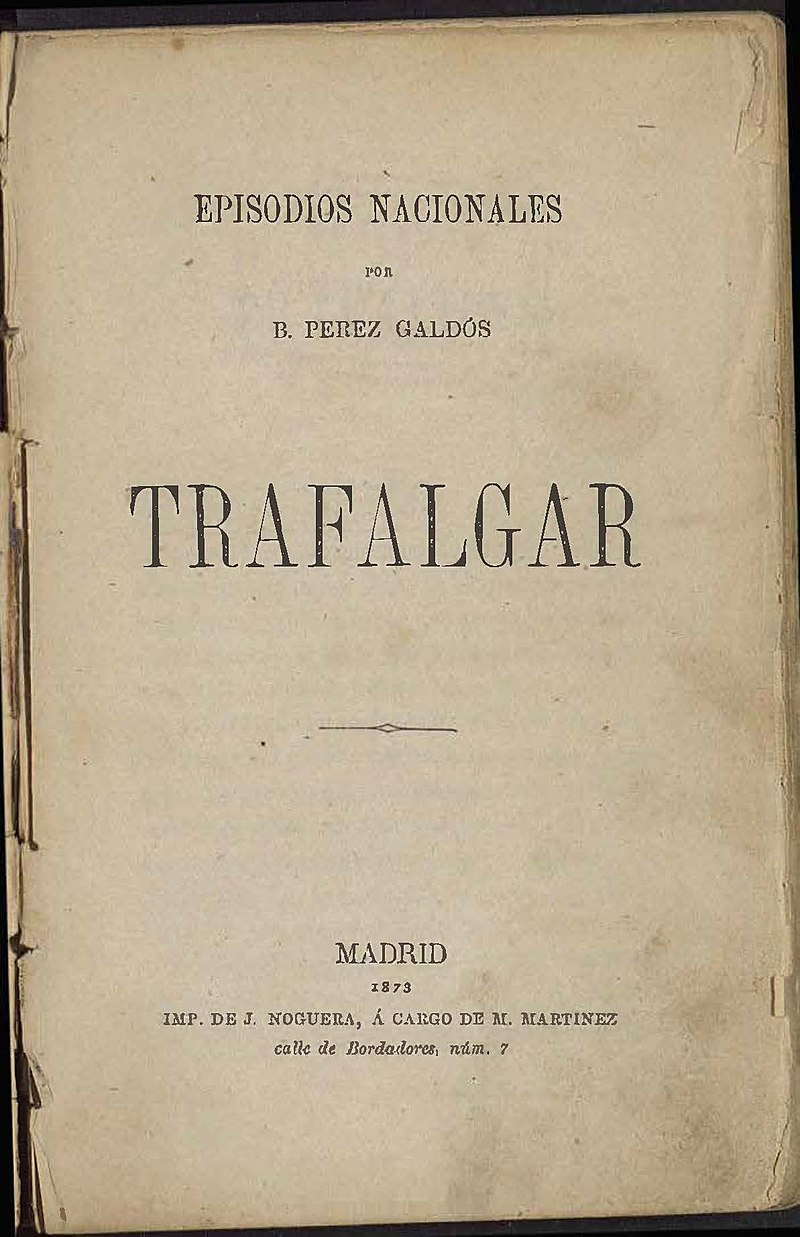
\includegraphics[height=300px]{Portada_Trafalgar_(1873).jpg}
\end{figure}

El dataset a utilizar consistirá en un archivo de texto con el contenido
íntegro en castellano de Trafalgar, disponible de manera libre en la
página de \href{https://www.gutenberg.org}{Project Gutenberg}. Asimismo,
como apartado optativo en este laboratorio se pueden utilizar otras
fuentes de texto. Aquí podéis descargar los datos a utilizar de El
Quijote y un par de obras adicionales:

\href{https://onedrive.live.com/download?cid=C506CF0A4F373B0F&resid=C506CF0A4F373B0F\%219424&authkey=AH0gb-qSo5Xd7Io}{El
ingenioso hidalgo Don Quijote de la Mancha (Miguel de Cervantes)}

\href{https://onedrive.live.com/download?cid=C506CF0A4F373B0F&resid=C506CF0A4F373B0F\%219433&authkey=AKvGD6DC3IRBqmc}{Compilación
de obras teatrales (Calderón de la Barca)}

\href{https://onedrive.live.com/download?cid=C506CF0A4F373B0F&resid=C506CF0A4F373B0F\%219434&authkey=AErPCAtMKOI5tYQ}{Trafalgar
(Benito Pérez Galdós)}

Como ya deberíamos de estar acostumbrados en problemas de Machine
Learning, es importante echar un vistazo a los datos antes de empezar.

    \subsection{1. Carga y procesado del
texto}\label{carga-y-procesado-del-texto}

    Primero, vamos a descargar el libro e inspeccionar los datos. El fichero
a descargar es una versión en .txt del libro Trafalgar, a la cual se le
han borrado introducciones, licencias y otras secciones para dejarlo con
el contenido real de la novela.

    \begin{tcolorbox}[breakable, size=fbox, boxrule=1pt, pad at break*=1mm, colback=white,colframe=black]
\begin{Verbatim}[commandchars=\\\{\}]
\PY{k+kn}{import} \PY{n+nn}{numpy} \PY{k}{as} \PY{n+nn}{np}
\PY{k+kn}{import} \PY{n+nn}{keras}
\PY{k+kn}{import} \PY{n+nn}{matplotlib}\PY{n+nn}{.}\PY{n+nn}{pyplot} \PY{k}{as} \PY{n+nn}{plt}
\PY{k+kn}{from} \PY{n+nn}{keras}\PY{n+nn}{.}\PY{n+nn}{callbacks} \PY{k+kn}{import} \PY{n}{LambdaCallback}
\PY{k+kn}{from} \PY{n+nn}{keras}\PY{n+nn}{.}\PY{n+nn}{models} \PY{k+kn}{import} \PY{n}{Sequential}
\PY{k+kn}{from} \PY{n+nn}{keras}\PY{n+nn}{.}\PY{n+nn}{layers} \PY{k+kn}{import} \PY{n}{Dense}
\PY{k+kn}{from} \PY{n+nn}{keras}\PY{n+nn}{.}\PY{n+nn}{layers} \PY{k+kn}{import} \PY{n}{Dropout}
\PY{k+kn}{from} \PY{n+nn}{keras}\PY{n+nn}{.}\PY{n+nn}{layers} \PY{k+kn}{import} \PY{n}{LSTM}
\PY{k+kn}{import} \PY{n+nn}{random}
\PY{k+kn}{import} \PY{n+nn}{io}
\PY{k+kn}{import} \PY{n+nn}{nltk}
\PY{n}{path} \PY{o}{=} \PY{n}{keras}\PY{o}{.}\PY{n}{utils}\PY{o}{.}\PY{n}{get\PYZus{}file}\PY{p}{(}
    \PY{n}{fname}\PY{o}{=}\PY{l+s+s2}{\PYZdq{}}\PY{l+s+s2}{Trafalgar.txt}\PY{l+s+s2}{\PYZdq{}}\PY{p}{,}
        \PY{n}{origin}\PY{o}{=}\PY{l+s+s2}{\PYZdq{}}\PY{l+s+s2}{https://onedrive.live.com/download?cid=C506CF0A4F373B0F\PYZam{}resid=C506CF0A4F373B0F}\PY{l+s+s2}{\PYZpc{}}\PY{l+s+s2}{219434\PYZam{}authkey=AErPCAtMKOI5tYQ}\PY{l+s+s2}{\PYZdq{}}\PY{p}{,}
        \PY{p}{)}
\end{Verbatim}
\end{tcolorbox}

    Una vez descargado, vamos a leer el contenido del fichero en una
variable. Adicionalmente, convertiremos el contenido del texto a
minúsculas para ponérselo un poco más fácil a nuestro modelo (de modo
que todas las letras sean minúsculas y el modelo no necesite diferenciar
entre minúsculas y mayúsculas).

\textbf{1.1.} Leer todo el contenido del fichero en una única variable
\textbf{\emph{text}} y convertir el string a minúsculas

    \begin{tcolorbox}[breakable, size=fbox, boxrule=1pt, pad at break*=1mm, colback=white,colframe=black]
\begin{Verbatim}[commandchars=\\\{\}]
\PY{n}{text}\PY{o}{=}\PY{n+nb}{open}\PY{p}{(}\PY{n}{path}\PY{p}{,} \PY{n}{encoding}\PY{o}{=}\PY{l+s+s2}{\PYZdq{}}\PY{l+s+s2}{utf8}\PY{l+s+s2}{\PYZdq{}}\PY{p}{)}\PY{o}{.}\PY{n}{read}\PY{p}{(}\PY{p}{)}\PY{o}{.}\PY{n}{lower}\PY{p}{(}\PY{p}{)}
\end{Verbatim}
\end{tcolorbox}

    Podemos comprobar ahora que efectivamente nuestra variable contiene el
resultado deseado, con el comienzo tan característico del Quijote.

    \begin{tcolorbox}[breakable, size=fbox, boxrule=1pt, pad at break*=1mm, colback=white,colframe=black]
\begin{Verbatim}[commandchars=\\\{\}]
\PY{n+nb}{print}\PY{p}{(}\PY{l+s+s2}{\PYZdq{}}\PY{l+s+s2}{Longitud del texto: }\PY{l+s+si}{\PYZob{}\PYZcb{}}\PY{l+s+s2}{\PYZdq{}}\PY{o}{.}\PY{n}{format}\PY{p}{(}\PY{n+nb}{len}\PY{p}{(}\PY{n}{text}\PY{p}{)}\PY{p}{)}\PY{p}{)}
\PY{n+nb}{print}\PY{p}{(}\PY{n}{text}\PY{p}{[}\PY{l+m+mi}{0}\PY{p}{:}\PY{l+m+mi}{300}\PY{p}{]}\PY{p}{)}
\end{Verbatim}
\end{tcolorbox}


\begin{tcolorbox}[breakable, size=fbox, boxrule=1pt, pad at break*=1mm,colback=cellbackground, colframe=cellborder]
    \begin{Verbatim}[commandchars=\\\{\}]
Longitud del texto: 300039
-i-
    \end{Verbatim}
\end{tcolorbox}

\begin{Verbatim}[commandchars=\\\{\}]

se me permitirá que antes de referir el gran suceso de que fui testigo,
diga algunas palabras sobre mi infancia, explicando por qué extraña
manera me llevaron los azares de la vida a presenciar la terrible
catástrofe de nuestra marina.

al hablar de mi nacimiento, no imitaré a la mayor parte de
    \end{Verbatim}

    \subsection{2. Procesado de los datos}\label{procesado-de-los-datos}

    Una de las grandes ventajas de trabajar con modelos que utilizan
caracteres en vez de palabras es que no necesitamos tokenizar el texto
(partirlo palabra a palabra). Nuestro modelo funcionará directamente con
los caracteres en el texto, incluyendo espacios, saltos de línea, etc.

Antes de hacer nada, necesitamos procesar el texto en entradas y salidas
compatibles con nuestro modelo. Como sabemos, un modelo del lenguaje con
RNNs acepta una serie de caracteres y predice el siguiente carácter en
la secuencia.

\begin{itemize}
\tightlist
\item
  ``\emph{Se me permitirá que antes de referir el gr}'' -\textgreater{}
  predicción: \textbf{a}
\item
  ``\emph{e me permitirá que antes de referir el gra}'' -\textgreater{}
  predicción: \textbf{n}
\end{itemize}

De modo que la entrada y la salida de nuestro modelo necesita ser algo
parecido a este esquema. En este punto, podríamos usar dos formas de
preparar los datos para nuestro modelo.

\begin{enumerate}
\def\labelenumi{\arabic{enumi}.}
\tightlist
\item
  \textbf{Secuencia a secuencia}. La entrada de nuestro modelo sería una
  secuencia y la salida sería esa secuencia trasladada un caracter a la
  derecha, de modo que en cada instante de tiempo la RNN tiene que
  predecir el carácter siguiente. Por ejemplo:
\end{enumerate}

\begin{quote}
\begin{itemize}
\tightlist
\item
  \emph{Input}: Se me permitirá que antes de referir el gr
\item
  \emph{Output}: e me permitirá que antes de referir el gra
\end{itemize}
\end{quote}

\begin{enumerate}
\def\labelenumi{\arabic{enumi}.}
\setcounter{enumi}{1}
\tightlist
\item
  \textbf{Secuencia a carácter}. En este variante, pasaríamos una
  secuencia de caracteres por nuestra RNN y, al llegar al final de la
  secuencia, predeciríamos el siguiente carácter.
\end{enumerate}

\begin{quote}
\begin{itemize}
\tightlist
\item
  \emph{Input}: Se me permitirá que antes de referir el gr
\item
  \emph{Output}: a
\end{itemize}
\end{quote}

En este laboratorio, por simplicidad, vamos a utilizar la segunda
variante (PERO USANDO PALABRAS NO CARACTERES).

De este modo, a partir del texto, hemos de generar nuestro propio
training data que consista en secuencias de PALABRAS con la siguiente
PALABRA a predecir. Para estandarizar las cosas, utilizaremos secuencias
de tamaño \emph{SEQ\_LENGTH} PALABRAS (un hiperparámetro que podemos
elegir nosotros).

    \paragraph{2.1. Obtención de las palabras y mapas de
palabras}\label{obtenciuxf3n-de-las-palabras-y-mapas-de-palabras}

Antes que nada, necesitamos saber qué palabras aparecen en el texto, ya
que tendremos que diferenciarlos mediante un índice de 0 a
\emph{num\_words} - 1 en el modelo. Obtener:

\begin{enumerate}
\def\labelenumi{\arabic{enumi}.}
\tightlist
\item
  Número de caracteres únicos que aparecen en el texto.
\item
  Diccionario que asocia char a índice único entre 0 y \emph{num\_words}
  - 1. Por ejemplo, \{`se': 0, `me': 1, \ldots\}
\item
  Diccionario reverso de índices a palabras: \{0: `se', 1: `me',
  \ldots\}
\end{enumerate}

    \begin{tcolorbox}[breakable, size=fbox, boxrule=1pt, pad at break*=1mm, colback=white,colframe=black]
\begin{Verbatim}[commandchars=\\\{\}]
\PY{n}{texto}\PY{o}{=}\PY{l+s+s2}{\PYZdq{}}\PY{l+s+s2}{\PYZdq{}}
\PY{k}{for} \PY{n}{letra} \PY{o+ow}{in} \PY{n}{text}\PY{p}{:}
    \PY{k}{if} \PY{o+ow}{not} \PY{n}{letra} \PY{o+ow}{in} \PY{l+s+s2}{\PYZdq{}}\PY{l+s+s2}{=\PYZgt{}\PYZlt{}*\PYZus{}?¿.,}\PY{l+s+s2}{\PYZsq{}}\PY{l+s+s2}{¡!()\PYZhy{}}\PY{l+s+si}{\PYZob{}\PYZcb{}}\PY{l+s+s2}{;[]»«:}\PY{l+s+se}{\PYZbs{}\PYZdq{}}\PY{l+s+s2}{\PYZdq{}}\PY{p}{:}
        \PY{n}{texto}\PY{o}{+}\PY{o}{=}\PY{n}{letra}
    \PY{n}{text}\PY{o}{=}\PY{n}{texto}

\PY{n}{palabras} \PY{o}{=} \PY{n}{text}\PY{o}{.}\PY{n}{split}\PY{p}{(}\PY{p}{)}
\PY{n}{palabras\PYZus{}unicas} \PY{o}{=} \PY{n+nb}{set}\PY{p}{(}\PY{n}{palabras}\PY{p}{)}
\PY{n}{word\PYZus{}index} \PY{o}{=} \PY{p}{\PYZob{}}\PY{p}{\PYZcb{}}
\PY{n}{reversed\PYZus{}index} \PY{o}{=} \PY{p}{\PYZob{}}\PY{p}{\PYZcb{}}
\PY{n}{k}\PY{o}{=}\PY{l+m+mi}{0}
\PY{k}{for} \PY{n}{palabra} \PY{o+ow}{in} \PY{n}{palabras\PYZus{}unicas}\PY{p}{:}
    \PY{n}{word\PYZus{}index}\PY{p}{[}\PY{n}{palabra}\PY{p}{]} \PY{o}{=} \PY{n}{k}
    \PY{n}{reversed\PYZus{}index}\PY{p}{[}\PY{n}{k}\PY{p}{]} \PY{o}{=} \PY{n}{palabra}
    \PY{n}{k}\PY{o}{+}\PY{o}{=}\PY{l+m+mi}{1}
\end{Verbatim}
\end{tcolorbox}

    \begin{tcolorbox}[breakable, size=fbox, boxrule=1pt, pad at break*=1mm, colback=white,colframe=black]
\begin{Verbatim}[commandchars=\\\{\}]
\PY{n+nb}{len}\PY{p}{(}\PY{n}{palabras\PYZus{}unicas}\PY{p}{)}
\end{Verbatim}
\end{tcolorbox}

\begin{tcolorbox}[breakable, size=fbox, boxrule=1pt, pad at break*=1mm,colback=cellbackground, colframe=cellborder]
\begin{Verbatim}[commandchars=\\\{\}]
8688
\end{Verbatim}
\end{tcolorbox}
        
    \begin{tcolorbox}[breakable, size=fbox, boxrule=1pt, pad at break*=1mm, colback=white,colframe=black]
\begin{Verbatim}[commandchars=\\\{\}]
\PY{n}{word\PYZus{}index}
\end{Verbatim}
\end{tcolorbox}

            \begin{tcolorbox}[breakable, size=fbox, boxrule=1pt, pad at break*=1mm,colback=cellbackground, colframe=cellborder]
\begin{Verbatim}[commandchars=\\\{\}]
\{'fruta': 0,
 'significar': 1,
 'coleto': 2,
 'apocamiento': 3,
 'hice': 4,
 'entibiaba': 5,
 'sargento': 6,
 'aparente': 7,
 'encopetados': 8,
 'busqué': 9,
 'mudo': 10,
 'datos': 11,
 'cuándo': 12,
 'entrometa': 13,
 'contestó': 14,
 'compramos': 15,
 'desencadenó': 16,
 'recrudecimiento': 17,
 'conociéramos': 18,
 'carena': 19,
 'resultados': 20,
 'éstos': 21,
 'cordero': 22,
 'castaña': 23,
 'conocerá': 24,
 'reñido': 25,
 'apto': 26,
 'fiestas': 27,
 'largamente': 28,
 'marché': 29,
 'novena': 30,
 'baile': 31,
 'pretendía': 32,
 'serios': 33,
 'comparativamente': 34,
 'entraremos': 35,
 'sequedad': 36,
 'crueldades': 37,
 'hallándome': 38,
 'desahogo': 39,
 'ochenta': 40,
 'agilidad': 41,
 'civil': 42,
 'cerró': 43,
 'marchar': 44,
 'maniobrar': 45,
 'amada': 46,
 'argumosa': 47,
 'malestar': 48,
 'edad': 49,
 'scipion': 50,
 'apreciarlo': 51,
 'zapatos': 52,
 'arreglaban': 53,
 'envolviéndonos': 54,
 'pecadillos': 55,
 'ahogados': 56,
 'estrechaba': 57,
 'apresados': 58,
 'despertar': 59,
 'cuantimás': 60,
 'perece': 61,
 'firme': 62,
 'mandados': 63,
 'te': 64,
 'entorpecía': 65,
 'ensangrentada': 66,
 'únicos': 67,
 'puras': 68,
 'ciertos': 69,
 '1834': 70,
 'llegó': 71,
 'bolas': 72,
 'jesús': 73,
 'alcázar': 74,
 'precedió': 75,
 'dados': 76,
 'expirar': 77,
 'apegado': 78,
 'bendito': 79,
 'segados': 80,
 'habré': 81,
 'diviertan': 82,
 'antigua': 83,
 'reinaba': 84,
 'perezoso': 85,
 'sepultarnos': 86,
 'vuelven': 87,
 '|redoutablef': 88,
 'públicas': 89,
 'geología': 90,
 'castiguen': 91,
 'benévolo': 92,
 'suplicaron': 93,
 'avemaría': 94,
 'aguardaba': 95,
 'castigaría': 96,
 'enorme': 97,
 'perplejidad': 98,
 'boca': 99,
 'defendernos': 100,
 'barras': 101,
 'paraíso': 102,
 'x': 103,
 'apretamos': 104,
 'malísima': 105,
 'luengo': 106,
 'habiéndose': 107,
 'pensaras': 108,
 'grandezas': 109,
 'navales': 110,
 'palabra': 111,
 'rendir': 112,
 'mostrando': 113,
 'realidad': 114,
 'grilla': 115,
 'trastorno': 116,
 'descarga': 117,
 'verme': 118,
 'arias': 119,
 'despabilado': 120,
 'andalucía': 121,
 'ninguno': 122,
 'buscarla': 123,
 'retirándose': 124,
 'previo': 125,
 'afectaba': 126,
 'soplaron': 127,
 'caballerosidad': 128,
 'media': 129,
 'terribles': 130,
 'maistral': 131,
 'daban': 132,
 'episodio': 133,
 'todas': 134,
 'aplanándose': 135,
 'fatal': 136,
 'romper': 137,
 'pajes': 138,
 'concierto': 139,
 'talladas': 140,
 'cascarilla': 141,
 'contestarme': 142,
 'acudí': 143,
 'posible': 144,
 'procedencias': 145,
 'consternación': 146,
 'carecían': 147,
 'alzar': 148,
 'quejó': 149,
 'infinitas': 150,
 'guerra': 151,
 'reunidos': 152,
 'conservación': 153,
 'calurosa': 154,
 'diera': 155,
 'lastimero': 156,
 'hallaron': 157,
 'dolorido': 158,
 'respiraron': 159,
 'nosotros': 160,
 'evitado': 161,
 'faltado': 162,
 'holgazana': 163,
 'perdidos': 164,
 'tambiénmanifesté': 165,
 'exclamación': 166,
 'alegrorepuso': 167,
 'armas': 168,
 'apresarnos': 169,
 'populosas': 170,
 'trataban': 171,
 'reliquia': 172,
 'formadas': 173,
 'sarcófago': 174,
 'acurrucado': 175,
 'repercutía': 176,
 'mi': 177,
 'montados': 178,
 'ponerse': 179,
 'mandando': 180,
 'propicia': 181,
 'ocasionó': 182,
 'instante': 183,
 'rica': 184,
 'paca': 185,
 'atenciones': 186,
 'entristeció': 187,
 'altar': 188,
 'sentó': 189,
 'alcanza': 190,
 'nadie': 191,
 'imprevista': 192,
 'prudentes': 193,
 'sonar': 194,
 'culta': 195,
 'reflexiones': 196,
 'ungüentos': 197,
 'basta': 198,
 'combustibles': 199,
 'rudo': 200,
 'batahola': 201,
 'aventurarme': 202,
 'duele': 203,
 'sirvo': 204,
 'andaluz': 205,
 'considerando': 206,
 'muñequito': 207,
 'importantes': 208,
 'esperanza': 209,
 'expuso': 210,
 'anoche': 211,
 'fingido': 212,
 'proyectos': 213,
 'último': 214,
 'pajarillas': 215,
 'plinmuf': 216,
 'largo': 217,
 'particulares': 218,
 'olé': 219,
 'ahdije': 220,
 'mezquinamente': 221,
 'varón': 222,
 'duplicar': 223,
 'infundido': 224,
 'corto': 225,
 'churruca': 226,
 'gases': 227,
 '|intrépide': 228,
 'consignó': 229,
 'verde': 230,
 'huían': 231,
 'pieles': 232,
 'riñó': 233,
 'aprecia': 234,
 'gabacho': 235,
 'taché': 236,
 'demostración': 237,
 'ventura': 238,
 'encina': 239,
 'continente': 240,
 'decoro': 241,
 'entró': 242,
 'tapar': 243,
 'bulle': 244,
 'mares': 245,
 'eludí': 246,
 'atajándole': 247,
 'muerto': 248,
 'menester': 249,
 'vejer': 250,
 'ladrón': 251,
 'ajeno': 252,
 'trabuco': 253,
 'periodo': 254,
 'disipa': 255,
 'salada': 256,
 'conciencia': 257,
 'luces': 258,
 'sabido': 259,
 'estaré': 260,
 '++': 261,
 'suspicacia': 262,
 'considerarse': 263,
 'sentimiento': 264,
 'encerraba': 265,
 'vencer': 266,
 'serené': 267,
 'compleja': 268,
 'simples': 269,
 'ahogan': 270,
 'efecto': 271,
 'ansiedad': 272,
 'marineras': 273,
 'sostén': 274,
 'modificara': 275,
 'cebaron': 276,
 'comprende': 277,
 'tengo': 278,
 'formidable': 279,
 'magnánimos': 280,
 'arriar': 281,
 'encantadora': 282,
 'mahón': 283,
 'pasó': 284,
 'consagrarte': 285,
 'propenso': 286,
 'corríamos': 287,
 'mediohombredecía': 288,
 'nodijo': 289,
 'oyera': 290,
 'mis': 291,
 'indicar': 292,
 'asegura': 293,
 'presentose': 294,
 'jactancioso': 295,
 'sainete': 296,
 '1796': 297,
 'colmó': 298,
 'seré': 299,
 'eché': 300,
 'espectáculo': 301,
 'desastredijo': 302,
 'comparable': 303,
 'físicos': 304,
 'límites': 305,
 'baladronadas': 306,
 'mire': 307,
 'pintado': 308,
 'pichón': 309,
 'tramo': 310,
 'remolcadora': 311,
 'armónico': 312,
 'próximamente': 313,
 'arrojaría': 314,
 'maniobra': 315,
 'pavimento': 316,
 'vagar': 317,
 'doméstico': 318,
 'apresadovive': 319,
 'ideadas': 320,
 'desmayados': 321,
 'nos': 322,
 'lluvia': 323,
 'relevado': 324,
 'imaginarse': 325,
 'con': 326,
 'oficialillo': 327,
 'representé': 328,
 'quedarme': 329,
 'muebles': 330,
 'imagen': 331,
 'sernos': 332,
 'felipe': 333,
 'porfía': 334,
 'afortunados': 335,
 'penetraba': 336,
 'grabados': 337,
 'atrocidades': 338,
 'fuese': 339,
 'mareado': 340,
 'ilustre': 341,
 'agarré': 342,
 'alarido': 343,
 'sacrificando': 344,
 'levanta': 345,
 'popa': 346,
 'cuida': 347,
 'patente': 348,
 'dices': 349,
 'retratista': 350,
 'ausencias': 351,
 'disparaba': 352,
 'íbamos': 353,
 'mulas': 354,
 'restañadas': 355,
 'asombraba': 356,
 'enemiga': 357,
 'lindamente': 358,
 'vocablo': 359,
 'tragos': 360,
 'piedad': 361,
 'pataplús': 362,
 'sacados': 363,
 'toda': 364,
 'seguía': 365,
 'hombredijo': 366,
 'mangas': 367,
 'extravío': 368,
 'asolando': 369,
 '30': 370,
 'respondo': 371,
 'cada': 372,
 'desembarco': 373,
 'conversaciones': 374,
 'etiqueta': 375,
 'alimento': 376,
 'abandonadas': 377,
 'sí': 378,
 'auxilios': 379,
 'paseamos': 380,
 'economizaba': 381,
 'veía': 382,
 'grave': 383,
 'cargamos': 384,
 'existe': 385,
 'decirlo': 386,
 'capaces': 387,
 'consejero': 388,
 'butrón': 389,
 'caritativa': 390,
 'acongojadas': 391,
 'columna': 392,
 'hallaban': 393,
 'ridiculeces': 394,
 'imperial': 395,
 'lucha': 396,
 'apostrofó': 397,
 'infiel': 398,
 'conducta': 399,
 'abrieron': 400,
 '116': 401,
 'apriétate': 402,
 'recalado': 403,
 '7murió': 404,
 'rondaba': 405,
 'año': 406,
 'advertir': 407,
 'añadió': 408,
 'dureza': 409,
 'criticado': 410,
 'churrucaexclamó': 411,
 'desaparecido': 412,
 'villeneuve': 413,
 'suelen': 414,
 'construido': 415,
 'desesperación': 416,
 'fardo': 417,
 'rato': 418,
 'nublaron': 419,
 'indica': 420,
 'exprofeso': 421,
 'útiles': 422,
 'queremos': 423,
 'agarrándose': 424,
 'inoportunamente': 425,
 'ustedes': 426,
 'colegía': 427,
 'me': 428,
 'disgustar': 429,
 'quedar': 430,
 'dimensiones': 431,
 'frontera': 432,
 'travesuras': 433,
 'avanzar': 434,
 '36': 435,
 'volvía': 436,
 'estampa': 437,
 'devolviendo': 438,
 'océano': 439,
 'dominar': 440,
 'retribuido': 441,
 'hermanos': 442,
 'penetrar': 443,
 'perdí': 444,
 'inexplicable': 445,
 'altamente': 446,
 'consigna': 447,
 'carreras': 448,
 'agosto': 449,
 'frívolas': 450,
 'maravillaron': 451,
 'lentamente': 452,
 'yo': 453,
 'carlos': 454,
 'contramaestre': 455,
 'entrepuentes': 456,
 'enternidad': 457,
 'concertado': 458,
 'amo': 459,
 'alargaba': 460,
 'azotando': 461,
 'historia': 462,
 'buscar': 463,
 'injerido': 464,
 'marcarlos': 465,
 'destrozándose': 466,
 'decaimiento': 467,
 'caminos': 468,
 'explicando': 469,
 'poeta': 470,
 'significaba': 471,
 'oírla': 472,
 'londres': 473,
 'satisfacer': 474,
 'teñía': 475,
 'insignificante': 476,
 'primera': 477,
 'sujeto': 478,
 'deslizándose': 479,
 'tranquilizarme': 480,
 'abundancia': 481,
 'japón': 482,
 'distinguida': 483,
 'aumentando': 484,
 'extraordinarias': 485,
 'niño': 486,
 'trozos': 487,
 'extraño': 488,
 'pared': 489,
 'guardianes': 490,
 'balas': 491,
 'arbitrio': 492,
 'ana120': 493,
 'larguísima': 494,
 'hija': 495,
 'existía': 496,
 'volviese': 497,
 'martirizados': 498,
 'maderas': 499,
 '1775': 500,
 'soñar': 501,
 'restauración': 502,
 'contó': 503,
 'loco': 504,
 'asintieron': 505,
 'inclinándose': 506,
 'cesaron': 507,
 'creen': 508,
 'sistemática': 509,
 'vergüenza': 510,
 'solía': 511,
 'estásdijo': 512,
 'rápido': 513,
 'rosario': 514,
 'imperiosa': 515,
 'monsieur': 516,
 'discurrí': 517,
 'comunicándose': 518,
 'saber': 519,
 'hermenegildo': 520,
 'voluble': 521,
 'violentamente': 522,
 'levantarse': 523,
 'algazara': 524,
 'honradamente': 525,
 'dormido': 526,
 'mostrándome': 527,
 'levantamos': 528,
 'aquéllas': 529,
 'pueblos': 530,
 'el2': 531,
 'cargo': 532,
 'agobia': 533,
 'apresaban': 534,
 'hueca': 535,
 'llamaban': 536,
 'servicios': 537,
 'banqueta': 538,
 'diálogo': 539,
 'declamación': 540,
 'arenga': 541,
 'herejes': 542,
 'precipitó': 543,
 'atmósfera': 544,
 'miraban': 545,
 'esperaba': 546,
 'contener': 547,
 'pública': 548,
 'quiero': 549,
 'pesadumbres': 550,
 'ciegas': 551,
 'adquirió': 552,
 'fraternalmente': 553,
 'transparentar': 554,
 'alcé': 555,
 'infundíamos': 556,
 'herir': 557,
 'marchaban': 558,
 'par': 559,
 'bailasen': 560,
 'inválido': 561,
 'baluarte': 562,
 'procedió': 563,
 'pesada': 564,
 'puesto': 565,
 'lindísima': 566,
 'abate': 567,
 'fijo': 568,
 'amanecido': 569,
 'yoañadió': 570,
 'extremadamente': 571,
 'siendo': 572,
 'desastres': 573,
 'diciéndoles': 574,
 'recibió': 575,
 'evadí': 576,
 'humanas': 577,
 'valeroso': 578,
 'ocurrencia': 579,
 'amabilidades': 580,
 'confesarse': 581,
 'advirtiéndola': 582,
 'llevaba': 583,
 'despertó': 584,
 'puse': 585,
 'vale': 586,
 'escuchaba': 587,
 'víctimas': 588,
 'principios': 589,
 'tambiéndijo': 590,
 'rescatar': 591,
 'parecidos': 592,
 'desocupadas': 593,
 'ininteligible': 594,
 'aparecieron': 595,
 'ciega': 596,
 'asocio': 597,
 'cañones': 598,
 'mercedes': 599,
 'entramos': 600,
 'lamentó': 601,
 'ordinarios': 602,
 'preparaba': 603,
 'moños': 604,
 'dijo': 605,
 'escenas': 606,
 'trasbordamos': 607,
 'lobo': 608,
 'pescadillas': 609,
 'muevan': 610,
 'agita': 611,
 'magníficos': 612,
 'cola': 613,
 'esperar': 614,
 'ocurrida': 615,
 'pesado': 616,
 'fragancia': 617,
 'perecería': 618,
 'combina': 619,
 'treinta': 620,
 'pusieran': 621,
 'completos': 622,
 'viento': 623,
 'convencerla': 624,
 'neptuno': 625,
 'izada': 626,
 'melancólico': 627,
 'disparaban': 628,
 'echaban': 629,
 'perdoné': 630,
 'mudos': 631,
 'rapacidad': 632,
 'derrotado': 633,
 'salida': 634,
 'remontara': 635,
 'transfiguración': 636,
 'abracé': 637,
 'encallar': 638,
 'amiguito': 639,
 'origen': 640,
 'insultando': 641,
 'extraordinariamente': 642,
 'atendí': 643,
 'hablara': 644,
 'casado': 645,
 'ocurridos': 646,
 'digna': 647,
 '|achilles': 648,
 'probar': 649,
 'baldeo': 650,
 'llegar': 651,
 'oficiales': 652,
 'ahínco': 653,
 'vaivén': 654,
 'perecieran': 655,
 'aspirando': 656,
 'ordenándome': 657,
 'cuentascontestó': 658,
 'arreciado': 659,
 'trasbordo': 660,
 'llego': 661,
 'cambiaban': 662,
 'cabeza': 663,
 'representaba': 664,
 'quise': 665,
 'ejemplar': 666,
 'cuidarse': 667,
 'prince': 668,
 'personalizarlos': 669,
 'auxiliarla': 670,
 'olas': 671,
 'secundase': 672,
 'peregrinos': 673,
 'decíamos': 674,
 'encontrábamos': 675,
 'coronel': 676,
 'rotundamente': 677,
 'dilatado': 678,
 'moral': 679,
 'cristal': 680,
 'descalabro': 681,
 'agasajo': 682,
 'hueso': 683,
 'pensó': 684,
 'secretaría': 685,
 'escorzaba': 686,
 'ángeles': 687,
 'trasladarme': 688,
 'intenta': 689,
 'pulgada': 690,
 'pusieron': 691,
 'aplacadas': 692,
 'gabriel': 693,
 'escuadras': 694,
 'estadística': 695,
 'picón': 696,
 'contentó': 697,
 'reunían': 698,
 'gritando': 699,
 'hubiera': 700,
 'arrebato': 701,
 'rematarnos': 702,
 'atrozmente': 703,
 'alternando': 704,
 'quitármela': 705,
 'fundada': 706,
 'fogonazo': 707,
 'caliente': 708,
 'avanza': 709,
 'muere': 710,
 'matan': 711,
 'locuras': 712,
 'revolvía': 713,
 'comprendió': 714,
 'añada': 715,
 'alegres': 716,
 'colilla': 717,
 'libren': 718,
 'señoría': 719,
 'conoce': 720,
 'oficialidad': 721,
 'partes': 722,
 'alumnos': 723,
 'tan': 724,
 'emparentada': 725,
 'peligrosos': 726,
 'trastorna': 727,
 'jaula': 728,
 '3': 729,
 'reparos': 730,
 'absuelva': 731,
 '|trinidad': 732,
 'ojos': 733,
 'cubrir': 734,
 'murallas': 735,
 'austria': 736,
 'consistía': 737,
 'descendía': 738,
 'escolares': 739,
 'lograron': 740,
 'enfilarla': 741,
 'denodadamente': 742,
 'codo': 743,
 'martinica': 744,
 'sonado': 745,
 'darme': 746,
 'damas': 747,
 'direcciones': 748,
 'cuatrocientos': 749,
 'cuántas': 750,
 'entregara': 751,
 'magon': 752,
 'ágiles': 753,
 'explicó': 754,
 'afluía': 755,
 'gavia': 756,
 'excitando': 757,
 'echármele': 758,
 'notar': 759,
 'peripecias': 760,
 'mortales': 761,
 'desplegar': 762,
 'arrodillé': 763,
 'alta': 764,
 'embarco': 765,
 'ordinariamente': 766,
 'esas': 767,
 'para': 768,
 'pálido': 769,
 'primeros': 770,
 'zascandil': 771,
 'estribo': 772,
 'acompañando': 773,
 'dejé': 774,
 'diestro': 775,
 'pardo': 776,
 'momentos': 777,
 'castigado': 778,
 'destacaba': 779,
 'grupo': 780,
 'pescozón': 781,
 'cuidé': 782,
 'indefinible': 783,
 'confusión': 784,
 'va': 785,
 'descubierta': 786,
 'tantas': 787,
 'buenocontestó': 788,
 'm': 789,
 'decían': 790,
 'encaré': 791,
 'ejecutando': 792,
 'probarla': 793,
 'comprendí': 794,
 'desatose': 795,
 'permiso': 796,
 'apagado': 797,
 'apéndice': 798,
 'guatemala': 799,
 'dramáticas': 800,
 'horrible': 801,
 'atrasada': 802,
 'vicente': 803,
 'fiera': 804,
 'combinadadijo': 805,
 'reparar': 806,
 'sublime': 807,
 'amojamado': 808,
 'compadrele': 809,
 'terreno': 810,
 'distinto': 811,
 'respirábamos': 812,
 'designó': 813,
 'dudo': 814,
 'dejaron': 815,
 'cansar': 816,
 'consagráronle': 817,
 'oyendo': 818,
 'enseñáronme': 819,
 'evidente': 820,
 'restablecer': 821,
 'comestibles': 822,
 'muera': 823,
 'señoras': 824,
 'repitió': 825,
 'centro': 826,
 'aprendí': 827,
 'movimiento': 828,
 'presentarme': 829,
 'retardar': 830,
 'presentó': 831,
 'vacíos': 832,
 'turbada': 833,
 'línea': 834,
 'remolcar': 835,
 'aljofifa': 836,
 'pergenio': 837,
 'parezcamos': 838,
 'quiebran': 839,
 'hueco': 840,
 'débiles': 841,
 'remolcado': 842,
 'puerta': 843,
 'diferenciaba': 844,
 'llegaremospregunté': 845,
 'impulsado': 846,
 'monarca': 847,
 'realzado': 848,
 'puedes': 849,
 'fueran': 850,
 'prestaba': 851,
 'delicados': 852,
 'gana': 853,
 'aventurado': 854,
 'tablones': 855,
 'marinerillos': 856,
 'centelleantes': 857,
 'órdenes': 858,
 'todavía': 859,
 'disparado': 860,
 'déjalesme': 861,
 'burros': 862,
 'evitarles': 863,
 'llamarse': 864,
 'pierde': 865,
 'soplaba': 866,
 'agresión': 867,
 'creocontesté': 868,
 'cumplido': 869,
 'inventopues': 870,
 'referidas': 871,
 'emociones': 872,
 'anocheció': 873,
 'represando': 874,
 'canciones': 875,
 'asociaba': 876,
 'hacen': 877,
 'golpes': 878,
 'bonitos': 879,
 'cuya': 880,
 'inventiva': 881,
 'celebraron': 882,
 'creyendo': 883,
 'entrar': 884,
 'tendrías': 885,
 'ardientes': 886,
 'lucí': 887,
 'gallardo': 888,
 'enumerar': 889,
 'extinguido': 890,
 'serenidad': 891,
 'observara': 892,
 'alegrara': 893,
 'caudales': 894,
 'desaliento': 895,
 'interrogué': 896,
 'buenos': 897,
 'combés': 898,
 'figura': 899,
 'palpita': 900,
 'día': 901,
 'corrí': 902,
 'inflamándose': 903,
 'sucedieron': 904,
 'transforma': 905,
 'seis': 906,
 'sirviendo': 907,
 'conducido': 908,
 'lado': 909,
 'dejando': 910,
 'coraje': 911,
 'flora': 912,
 'averías': 913,
 'caí': 914,
 'ámbito': 915,
 'sollados': 916,
 'chaleco': 917,
 'incansable': 918,
 'auxiliaran': 919,
 'melancolía': 920,
 'restos': 921,
 'salir': 922,
 'cabezas': 923,
 'días': 924,
 'sistema': 925,
 'tiro': 926,
 'eclipse': 927,
 'frescura': 928,
 'existencia': 929,
 'conmovido': 930,
 'juzgarme': 931,
 'siete': 932,
 'diversas': 933,
 'providencia': 934,
 'negro': 935,
 'crucero': 936,
 'o': 937,
 'indiferente': 938,
 'ahogamos': 939,
 'escuché': 940,
 'balandra': 941,
 'quiere': 942,
 'santo': 943,
 'necesitasen': 944,
 'ineptitud': 945,
 'amargamente': 946,
 'cabellos': 947,
 'derrotados': 948,
 'empezar': 949,
 'haciéndome': 950,
 'incapaz': 951,
 'arrastra': 952,
 'andaría': 953,
 'posibles': 954,
 'misma': 955,
 'henchirse': 956,
 'murieron': 957,
 'proezas': 958,
 'encendido': 959,
 'hacerme': 960,
 'apresar': 961,
 'siguiendo': 962,
 'campanas': 963,
 'ávidos': 964,
 'caracoles': 965,
 'distábamos': 966,
 'fatigado': 967,
 'contrabandistas': 968,
 'interesantes': 969,
 'sotaventó': 970,
 'nadando': 971,
 'proyectillo': 972,
 'obsequiarles': 973,
 'extraña': 974,
 'embriagarse': 975,
 'dando': 976,
 'hacia': 977,
 'sexta': 978,
 'r': 979,
 'lazos': 980,
 'bastaban': 981,
 'miré': 982,
 'américa': 983,
 'bofetón': 984,
 'inoportunidad': 985,
 'pena': 986,
 'arguyéndole': 987,
 'falúa': 988,
 'agarraban': 989,
 'usaba': 990,
 'perdiste': 991,
 'rocas': 992,
 'pascuas': 993,
 'madrid': 994,
 'confesar': 995,
 'zurra': 996,
 'remolcados': 997,
 'acercaba': 998,
 'quizás': 999,
 {\ldots}\}
\end{Verbatim}
\end{tcolorbox}
        
    \paragraph{2.2. Obtención de secuencias de entrada y palabra a
predecir}\label{obtenciuxf3n-de-secuencias-de-entrada-y-palabra-a-predecir}

Ahora, vamos a obtener las secuencias de entrada en formato texto y las
correspondientes palabras a predecir. Para ello, recorrer el texto
completo leído anteriormente, obteniendo una secuencia de SEQ\_LENGTH
palabras y la siguiente palabra a predecir. Una vez hecho, desplazarse
una palabra a la derecha y hacer lo mismo para obtener una nueva
secuencia y predicción. Guardar las secuencias en una variable
\textbf{\emph{sequences}} y las palabras a predecir en una variable
\textbf{\emph{next\_words}}.

Por ejemplo, si el texto fuera ``Don Quijote'' y SEQ\_LENGTH fuese 2,
tendríamos

\begin{itemize}
\tightlist
\item
  \emph{sequences} = {[}``Don Quijote'', ``Quijote de''{]}
\item
  \emph{next\_chars} = {[}`de', `La'{]}
\end{itemize}

    \begin{tcolorbox}[breakable, size=fbox, boxrule=1pt, pad at break*=1mm, colback=white,colframe=black]
\begin{Verbatim}[commandchars=\\\{\}]
\PY{c+c1}{\PYZsh{} Definimos el tamaño de las secuencias. Puedes dejar este valor por defecto.}
\PY{n}{SEQ\PYZus{}LENGTH} \PY{o}{=} \PY{l+m+mi}{5}
\PY{n}{NUM\PYZus{}WORDS} \PY{o}{=} \PY{n+nb}{len}\PY{p}{(}\PY{n}{palabras\PYZus{}unicas}\PY{p}{)}

\PY{n}{step}\PY{o}{=}\PY{l+m+mi}{1}
\PY{n}{sequences} \PY{o}{=} \PY{p}{[}\PY{p}{]}
\PY{n}{next\PYZus{}words} \PY{o}{=} \PY{p}{[}\PY{p}{]}
\end{Verbatim}
\end{tcolorbox}

    Indicar el tamaño del training set que acabamos de generar.

    \begin{tcolorbox}[breakable, size=fbox, boxrule=1pt, pad at break*=1mm, colback=white,colframe=black]
\begin{Verbatim}[commandchars=\\\{\}]
\PY{k}{for} \PY{n}{i} \PY{o+ow}{in} \PY{n+nb}{range}\PY{p}{(}\PY{l+m+mi}{0}\PY{p}{,}\PY{n+nb}{len}\PY{p}{(}\PY{n}{palabras}\PY{p}{)}\PY{o}{\PYZhy{}}\PY{n}{SEQ\PYZus{}LENGTH}\PY{p}{,} \PY{n}{step}\PY{p}{)}\PY{p}{:}
    \PY{n}{sequences}\PY{o}{.}\PY{n}{append}\PY{p}{(}\PY{n}{palabras}\PY{p}{[}\PY{n}{i}\PY{p}{:}\PY{n}{i}\PY{o}{+}\PY{n}{SEQ\PYZus{}LENGTH}\PY{p}{]}\PY{p}{)}
    \PY{n}{next\PYZus{}words}\PY{o}{.}\PY{n}{append}\PY{p}{(}\PY{n}{palabras}\PY{p}{[}\PY{n}{i}\PY{o}{+}\PY{n}{SEQ\PYZus{}LENGTH}\PY{p}{]}\PY{p}{)}
\end{Verbatim}
\end{tcolorbox}

    \begin{tcolorbox}[breakable, size=fbox, boxrule=1pt, pad at break*=1mm, colback=white,colframe=black]
\begin{Verbatim}[commandchars=\\\{\}]
\PY{n}{sequences}\PY{p}{[}\PY{l+m+mi}{8}\PY{p}{]}
\end{Verbatim}
\end{tcolorbox}

            \begin{tcolorbox}[breakable, size=fbox, boxrule=1pt, pad at break*=1mm,colback=cellbackground, colframe=cellborder]
\begin{Verbatim}[commandchars=\\\{\}]
['el', 'gran', 'suceso', 'de', 'que']
\end{Verbatim}
\end{tcolorbox}
        
    \begin{tcolorbox}[breakable, size=fbox, boxrule=1pt, pad at break*=1mm, colback=white,colframe=black]
\begin{Verbatim}[commandchars=\\\{\}]
\PY{n}{next\PYZus{}words}\PY{p}{[}\PY{l+m+mi}{8}\PY{p}{]}
\end{Verbatim}
\end{tcolorbox}

            \begin{tcolorbox}[breakable, size=fbox, boxrule=1pt, pad at break*=1mm,colback=cellbackground, colframe=cellborder]
\begin{Verbatim}[commandchars=\\\{\}]
'fui'
\end{Verbatim}
\end{tcolorbox}
        
    Como el Quijote es muy largo y tenemos muchas secuencias, podríamos
encontrar problemas de memoria. Por ello, vamos a elegir un número
máximo de ellas. Si estás corriendo esto localmente y tienes problemas
de memoria, puedes reducir el tamaño aún más, pero ten cuidado porque, a
menos datos, peor calidad del modelo.

    \begin{tcolorbox}[breakable, size=fbox, boxrule=1pt, pad at break*=1mm, colback=white,colframe=black]
\begin{Verbatim}[commandchars=\\\{\}]
\PY{n}{sequences}\PY{p}{[}\PY{n+nb}{len}\PY{p}{(}\PY{n}{sequences}\PY{p}{)}\PY{o}{\PYZhy{}}\PY{l+m+mi}{1}\PY{p}{]}
\end{Verbatim}
\end{tcolorbox}

            \begin{tcolorbox}[breakable, size=fbox, boxrule=1pt, pad at break*=1mm,colback=cellbackground, colframe=cellborder]
\begin{Verbatim}[commandchars=\\\{\}]
['ilustrada', 'por', 'enrique', 'y', 'arturo']
\end{Verbatim}
\end{tcolorbox}
        
    \begin{tcolorbox}[breakable, size=fbox, boxrule=1pt, pad at break*=1mm, colback=white,colframe=black]
\begin{Verbatim}[commandchars=\\\{\}]
\PY{n}{next\PYZus{}words}\PY{p}{[}\PY{n+nb}{len}\PY{p}{(}\PY{n}{sequences}\PY{p}{)}\PY{o}{\PYZhy{}}\PY{l+m+mi}{1}\PY{p}{]}
\end{Verbatim}
\end{tcolorbox}

            \begin{tcolorbox}[breakable, size=fbox, boxrule=1pt, pad at break*=1mm,colback=cellbackground, colframe=cellborder]
\begin{Verbatim}[commandchars=\\\{\}]
'mélida'
\end{Verbatim}
\end{tcolorbox}
        
    \begin{tcolorbox}[breakable, size=fbox, boxrule=1pt, pad at break*=1mm, colback=white,colframe=black]
\begin{Verbatim}[commandchars=\\\{\}]
\PY{c+c1}{\PYZsh{}Convertimos las sequencias en frases}
\PY{n}{frases} \PY{o}{=} \PY{p}{[}\PY{p}{]}
\PY{k}{for} \PY{n}{i} \PY{o+ow}{in} \PY{n+nb}{range}\PY{p}{(}\PY{n+nb}{len}\PY{p}{(}\PY{n}{sequences}\PY{p}{)}\PY{p}{)}\PY{p}{:}
    \PY{n}{frase} \PY{o}{=} \PY{l+s+s1}{\PYZsq{}}\PY{l+s+s1}{ }\PY{l+s+s1}{\PYZsq{}}\PY{o}{.}\PY{n}{join}\PY{p}{(}\PY{n}{sequences}\PY{p}{[}\PY{n}{i}\PY{p}{]}\PY{p}{)}
    \PY{n}{frases}\PY{o}{.}\PY{n}{append}\PY{p}{(}\PY{n}{frase}\PY{p}{)}
\PY{c+c1}{\PYZsh{}Tokenizar las frases}
\PY{n}{newsVec} \PY{o}{=} \PY{p}{[}\PY{n}{nltk}\PY{o}{.}\PY{n}{word\PYZus{}tokenize}\PY{p}{(}\PY{n}{frase}\PY{p}{,} \PY{n}{language}\PY{o}{=} \PY{l+s+s2}{\PYZdq{}}\PY{l+s+s2}{spanish}\PY{l+s+s2}{\PYZdq{}}\PY{p}{)} \PY{k}{for} \PY{n}{frase} \PY{o+ow}{in} \PY{n}{frases}\PY{p}{]}
\end{Verbatim}
\end{tcolorbox}

    \begin{tcolorbox}[breakable, size=fbox, boxrule=1pt, pad at break*=1mm, colback=white,colframe=black]
\begin{Verbatim}[commandchars=\\\{\}]
\PY{n}{newsVec}
\end{Verbatim}
\end{tcolorbox}

            \begin{tcolorbox}[breakable, size=fbox, boxrule=1pt, pad at break*=1mm,colback=cellbackground, colframe=cellborder]
\begin{Verbatim}[commandchars=\\\{\}]
[['i', 'se', 'me', 'permitirá', 'que'],
 ['se', 'me', 'permitirá', 'que', 'antes'],
 ['me', 'permitirá', 'que', 'antes', 'de'],
 ['permitirá', 'que', 'antes', 'de', 'referir'],
 ['que', 'antes', 'de', 'referir', 'el'],
 ['antes', 'de', 'referir', 'el', 'gran'],
 ['de', 'referir', 'el', 'gran', 'suceso'],
 ['referir', 'el', 'gran', 'suceso', 'de'],
 ['el', 'gran', 'suceso', 'de', 'que'],
 ['gran', 'suceso', 'de', 'que', 'fui'],
 ['suceso', 'de', 'que', 'fui', 'testigo'],
 ['de', 'que', 'fui', 'testigo', 'diga'],
 ['que', 'fui', 'testigo', 'diga', 'algunas'],
 ['fui', 'testigo', 'diga', 'algunas', 'palabras'],
 ['testigo', 'diga', 'algunas', 'palabras', 'sobre'],
 ['diga', 'algunas', 'palabras', 'sobre', 'mi'],
 ['algunas', 'palabras', 'sobre', 'mi', 'infancia'],
 ['palabras', 'sobre', 'mi', 'infancia', 'explicando'],
 ['sobre', 'mi', 'infancia', 'explicando', 'por'],
 ['mi', 'infancia', 'explicando', 'por', 'qué'],
 ['infancia', 'explicando', 'por', 'qué', 'extraña'],
 ['explicando', 'por', 'qué', 'extraña', 'manera'],
 ['por', 'qué', 'extraña', 'manera', 'me'],
 ['qué', 'extraña', 'manera', 'me', 'llevaron'],
 ['extraña', 'manera', 'me', 'llevaron', 'los'],
 ['manera', 'me', 'llevaron', 'los', 'azares'],
 ['me', 'llevaron', 'los', 'azares', 'de'],
 ['llevaron', 'los', 'azares', 'de', 'la'],
 ['los', 'azares', 'de', 'la', 'vida'],
 ['azares', 'de', 'la', 'vida', 'a'],
 ['de', 'la', 'vida', 'a', 'presenciar'],
 ['la', 'vida', 'a', 'presenciar', 'la'],
 ['vida', 'a', 'presenciar', 'la', 'terrible'],
 ['a', 'presenciar', 'la', 'terrible', 'catástrofe'],
 ['presenciar', 'la', 'terrible', 'catástrofe', 'de'],
 ['la', 'terrible', 'catástrofe', 'de', 'nuestra'],
 ['terrible', 'catástrofe', 'de', 'nuestra', 'marina'],
 ['catástrofe', 'de', 'nuestra', 'marina', 'al'],
 ['de', 'nuestra', 'marina', 'al', 'hablar'],
 ['nuestra', 'marina', 'al', 'hablar', 'de'],
 ['marina', 'al', 'hablar', 'de', 'mi'],
 ['al', 'hablar', 'de', 'mi', 'nacimiento'],
 ['hablar', 'de', 'mi', 'nacimiento', 'no'],
 ['de', 'mi', 'nacimiento', 'no', 'imitaré'],
 ['mi', 'nacimiento', 'no', 'imitaré', 'a'],
 ['nacimiento', 'no', 'imitaré', 'a', 'la'],
 ['no', 'imitaré', 'a', 'la', 'mayor'],
 ['imitaré', 'a', 'la', 'mayor', 'parte'],
 ['a', 'la', 'mayor', 'parte', 'de'],
 ['la', 'mayor', 'parte', 'de', 'los'],
 ['mayor', 'parte', 'de', 'los', 'que'],
 ['parte', 'de', 'los', 'que', 'cuentan'],
 ['de', 'los', 'que', 'cuentan', 'hechos'],
 ['los', 'que', 'cuentan', 'hechos', 'de'],
 ['que', 'cuentan', 'hechos', 'de', 'su'],
 ['cuentan', 'hechos', 'de', 'su', 'propia'],
 ['hechos', 'de', 'su', 'propia', 'vida'],
 ['de', 'su', 'propia', 'vida', 'quienes'],
 ['su', 'propia', 'vida', 'quienes', 'empiezan'],
 ['propia', 'vida', 'quienes', 'empiezan', 'nombrando'],
 ['vida', 'quienes', 'empiezan', 'nombrando', 'su'],
 ['quienes', 'empiezan', 'nombrando', 'su', 'parentela'],
 ['empiezan', 'nombrando', 'su', 'parentela', 'las'],
 ['nombrando', 'su', 'parentela', 'las', 'más'],
 ['su', 'parentela', 'las', 'más', 'veces'],
 ['parentela', 'las', 'más', 'veces', 'noble'],
 ['las', 'más', 'veces', 'noble', 'siempre'],
 ['más', 'veces', 'noble', 'siempre', 'hidalga'],
 ['veces', 'noble', 'siempre', 'hidalga', 'por'],
 ['noble', 'siempre', 'hidalga', 'por', 'lo'],
 ['siempre', 'hidalga', 'por', 'lo', 'menos'],
 ['hidalga', 'por', 'lo', 'menos', 'si'],
 ['por', 'lo', 'menos', 'si', 'no'],
 ['lo', 'menos', 'si', 'no', 'se'],
 ['menos', 'si', 'no', 'se', 'dicen'],
 ['si', 'no', 'se', 'dicen', 'descendientes'],
 ['no', 'se', 'dicen', 'descendientes', 'del'],
 ['se', 'dicen', 'descendientes', 'del', 'mismo'],
 ['dicen', 'descendientes', 'del', 'mismo', 'emperador'],
 ['descendientes', 'del', 'mismo', 'emperador', 'de'],
 ['del', 'mismo', 'emperador', 'de', 'trapisonda'],
 ['mismo', 'emperador', 'de', 'trapisonda', 'yo'],
 ['emperador', 'de', 'trapisonda', 'yo', 'en'],
 ['de', 'trapisonda', 'yo', 'en', 'esta'],
 ['trapisonda', 'yo', 'en', 'esta', 'parte'],
 ['yo', 'en', 'esta', 'parte', 'no'],
 ['en', 'esta', 'parte', 'no', 'puedo'],
 ['esta', 'parte', 'no', 'puedo', 'adornar'],
 ['parte', 'no', 'puedo', 'adornar', 'mi'],
 ['no', 'puedo', 'adornar', 'mi', 'libro'],
 ['puedo', 'adornar', 'mi', 'libro', 'con'],
 ['adornar', 'mi', 'libro', 'con', 'sonoros'],
 ['mi', 'libro', 'con', 'sonoros', 'apellidos'],
 ['libro', 'con', 'sonoros', 'apellidos', 'y'],
 ['con', 'sonoros', 'apellidos', 'y', 'fuera'],
 ['sonoros', 'apellidos', 'y', 'fuera', 'de'],
 ['apellidos', 'y', 'fuera', 'de', 'mi'],
 ['y', 'fuera', 'de', 'mi', 'madre'],
 ['fuera', 'de', 'mi', 'madre', 'a'],
 ['de', 'mi', 'madre', 'a', 'quien'],
 ['mi', 'madre', 'a', 'quien', 'conocí'],
 ['madre', 'a', 'quien', 'conocí', 'por'],
 ['a', 'quien', 'conocí', 'por', 'poco'],
 ['quien', 'conocí', 'por', 'poco', 'tiempo'],
 ['conocí', 'por', 'poco', 'tiempo', 'no'],
 ['por', 'poco', 'tiempo', 'no', 'tengo'],
 ['poco', 'tiempo', 'no', 'tengo', 'noticia'],
 ['tiempo', 'no', 'tengo', 'noticia', 'de'],
 ['no', 'tengo', 'noticia', 'de', 'ninguno'],
 ['tengo', 'noticia', 'de', 'ninguno', 'de'],
 ['noticia', 'de', 'ninguno', 'de', 'mis'],
 ['de', 'ninguno', 'de', 'mis', 'ascendientes'],
 ['ninguno', 'de', 'mis', 'ascendientes', 'si'],
 ['de', 'mis', 'ascendientes', 'si', 'no'],
 ['mis', 'ascendientes', 'si', 'no', 'es'],
 ['ascendientes', 'si', 'no', 'es', 'de'],
 ['si', 'no', 'es', 'de', 'adán'],
 ['no', 'es', 'de', 'adán', 'cuyo'],
 ['es', 'de', 'adán', 'cuyo', 'parentesco'],
 ['de', 'adán', 'cuyo', 'parentesco', 'me'],
 ['adán', 'cuyo', 'parentesco', 'me', 'parece'],
 ['cuyo', 'parentesco', 'me', 'parece', 'indiscutible'],
 ['parentesco', 'me', 'parece', 'indiscutible', 'doy'],
 ['me', 'parece', 'indiscutible', 'doy', 'principio'],
 ['parece', 'indiscutible', 'doy', 'principio', 'pues'],
 ['indiscutible', 'doy', 'principio', 'pues', 'a'],
 ['doy', 'principio', 'pues', 'a', 'mi'],
 ['principio', 'pues', 'a', 'mi', 'historia'],
 ['pues', 'a', 'mi', 'historia', 'como'],
 ['a', 'mi', 'historia', 'como', 'pablos'],
 ['mi', 'historia', 'como', 'pablos', 'el'],
 ['historia', 'como', 'pablos', 'el', 'buscón'],
 ['como', 'pablos', 'el', 'buscón', 'de'],
 ['pablos', 'el', 'buscón', 'de', 'segovia'],
 ['el', 'buscón', 'de', 'segovia', 'afortunadamente'],
 ['buscón', 'de', 'segovia', 'afortunadamente', 'dios'],
 ['de', 'segovia', 'afortunadamente', 'dios', 'ha'],
 ['segovia', 'afortunadamente', 'dios', 'ha', 'querido'],
 ['afortunadamente', 'dios', 'ha', 'querido', 'que'],
 ['dios', 'ha', 'querido', 'que', 'en'],
 ['ha', 'querido', 'que', 'en', 'esto'],
 ['querido', 'que', 'en', 'esto', 'sólo'],
 ['que', 'en', 'esto', 'sólo', 'nos'],
 ['en', 'esto', 'sólo', 'nos', 'parezcamos'],
 ['esto', 'sólo', 'nos', 'parezcamos', 'yo'],
 ['sólo', 'nos', 'parezcamos', 'yo', 'nací'],
 ['nos', 'parezcamos', 'yo', 'nací', 'en'],
 ['parezcamos', 'yo', 'nací', 'en', 'cádiz'],
 ['yo', 'nací', 'en', 'cádiz', 'y'],
 ['nací', 'en', 'cádiz', 'y', 'en'],
 ['en', 'cádiz', 'y', 'en', 'el'],
 ['cádiz', 'y', 'en', 'el', 'famoso'],
 ['y', 'en', 'el', 'famoso', 'barrio'],
 ['en', 'el', 'famoso', 'barrio', 'de'],
 ['el', 'famoso', 'barrio', 'de', 'la'],
 ['famoso', 'barrio', 'de', 'la', 'viña'],
 ['barrio', 'de', 'la', 'viña', 'que'],
 ['de', 'la', 'viña', 'que', 'no'],
 ['la', 'viña', 'que', 'no', 'es'],
 ['viña', 'que', 'no', 'es', 'hoy'],
 ['que', 'no', 'es', 'hoy', 'ni'],
 ['no', 'es', 'hoy', 'ni', 'menos'],
 ['es', 'hoy', 'ni', 'menos', 'era'],
 ['hoy', 'ni', 'menos', 'era', 'entonces'],
 ['ni', 'menos', 'era', 'entonces', 'academia'],
 ['menos', 'era', 'entonces', 'academia', 'de'],
 ['era', 'entonces', 'academia', 'de', 'buenas'],
 ['entonces', 'academia', 'de', 'buenas', 'costumbres'],
 ['academia', 'de', 'buenas', 'costumbres', 'la'],
 ['de', 'buenas', 'costumbres', 'la', 'memoria'],
 ['buenas', 'costumbres', 'la', 'memoria', 'no'],
 ['costumbres', 'la', 'memoria', 'no', 'me'],
 ['la', 'memoria', 'no', 'me', 'da'],
 ['memoria', 'no', 'me', 'da', 'luz'],
 ['no', 'me', 'da', 'luz', 'alguna'],
 ['me', 'da', 'luz', 'alguna', 'sobre'],
 ['da', 'luz', 'alguna', 'sobre', 'mi'],
 ['luz', 'alguna', 'sobre', 'mi', 'persona'],
 ['alguna', 'sobre', 'mi', 'persona', 'y'],
 ['sobre', 'mi', 'persona', 'y', 'mis'],
 ['mi', 'persona', 'y', 'mis', 'acciones'],
 ['persona', 'y', 'mis', 'acciones', 'en'],
 ['y', 'mis', 'acciones', 'en', 'la'],
 ['mis', 'acciones', 'en', 'la', 'niñez'],
 ['acciones', 'en', 'la', 'niñez', 'sino'],
 ['en', 'la', 'niñez', 'sino', 'desde'],
 ['la', 'niñez', 'sino', 'desde', 'la'],
 ['niñez', 'sino', 'desde', 'la', 'edad'],
 ['sino', 'desde', 'la', 'edad', 'de'],
 ['desde', 'la', 'edad', 'de', 'seis'],
 ['la', 'edad', 'de', 'seis', 'años'],
 ['edad', 'de', 'seis', 'años', 'y'],
 ['de', 'seis', 'años', 'y', 'si'],
 ['seis', 'años', 'y', 'si', 'recuerdo'],
 ['años', 'y', 'si', 'recuerdo', 'esta'],
 ['y', 'si', 'recuerdo', 'esta', 'fecha'],
 ['si', 'recuerdo', 'esta', 'fecha', 'es'],
 ['recuerdo', 'esta', 'fecha', 'es', 'porque'],
 ['esta', 'fecha', 'es', 'porque', 'la'],
 ['fecha', 'es', 'porque', 'la', 'asocio'],
 ['es', 'porque', 'la', 'asocio', 'a'],
 ['porque', 'la', 'asocio', 'a', 'un'],
 ['la', 'asocio', 'a', 'un', 'suceso'],
 ['asocio', 'a', 'un', 'suceso', 'naval'],
 ['a', 'un', 'suceso', 'naval', 'de'],
 ['un', 'suceso', 'naval', 'de', 'que'],
 ['suceso', 'naval', 'de', 'que', 'oí'],
 ['naval', 'de', 'que', 'oí', 'hablar'],
 ['de', 'que', 'oí', 'hablar', 'entonces'],
 ['que', 'oí', 'hablar', 'entonces', 'el'],
 ['oí', 'hablar', 'entonces', 'el', 'combate'],
 ['hablar', 'entonces', 'el', 'combate', 'del'],
 ['entonces', 'el', 'combate', 'del', 'cabo'],
 ['el', 'combate', 'del', 'cabo', 'de'],
 ['combate', 'del', 'cabo', 'de', 'san'],
 ['del', 'cabo', 'de', 'san', 'vicente'],
 ['cabo', 'de', 'san', 'vicente', 'acaecido'],
 ['de', 'san', 'vicente', 'acaecido', 'en'],
 ['san', 'vicente', 'acaecido', 'en', '1797'],
 ['vicente', 'acaecido', 'en', '1797', 'dirigiendo'],
 ['acaecido', 'en', '1797', 'dirigiendo', 'una'],
 ['en', '1797', 'dirigiendo', 'una', 'mirada'],
 ['1797', 'dirigiendo', 'una', 'mirada', 'hacia'],
 ['dirigiendo', 'una', 'mirada', 'hacia', 'lo'],
 ['una', 'mirada', 'hacia', 'lo', 'que'],
 ['mirada', 'hacia', 'lo', 'que', 'fue'],
 ['hacia', 'lo', 'que', 'fue', 'con'],
 ['lo', 'que', 'fue', 'con', 'la'],
 ['que', 'fue', 'con', 'la', 'curiosidad'],
 ['fue', 'con', 'la', 'curiosidad', 'y'],
 ['con', 'la', 'curiosidad', 'y', 'el'],
 ['la', 'curiosidad', 'y', 'el', 'interés'],
 ['curiosidad', 'y', 'el', 'interés', 'propios'],
 ['y', 'el', 'interés', 'propios', 'de'],
 ['el', 'interés', 'propios', 'de', 'quien'],
 ['interés', 'propios', 'de', 'quien', 'se'],
 ['propios', 'de', 'quien', 'se', 'observa'],
 ['de', 'quien', 'se', 'observa', 'imagen'],
 ['quien', 'se', 'observa', 'imagen', 'confusa'],
 ['se', 'observa', 'imagen', 'confusa', 'y'],
 ['observa', 'imagen', 'confusa', 'y', 'borrosa'],
 ['imagen', 'confusa', 'y', 'borrosa', 'en'],
 ['confusa', 'y', 'borrosa', 'en', 'el'],
 ['y', 'borrosa', 'en', 'el', 'cuadro'],
 ['borrosa', 'en', 'el', 'cuadro', 'de'],
 ['en', 'el', 'cuadro', 'de', 'las'],
 ['el', 'cuadro', 'de', 'las', 'cosas'],
 ['cuadro', 'de', 'las', 'cosas', 'pasadas'],
 ['de', 'las', 'cosas', 'pasadas', 'me'],
 ['las', 'cosas', 'pasadas', 'me', 'veo'],
 ['cosas', 'pasadas', 'me', 'veo', 'jugando'],
 ['pasadas', 'me', 'veo', 'jugando', 'en'],
 ['me', 'veo', 'jugando', 'en', 'la'],
 ['veo', 'jugando', 'en', 'la', 'caleta'],
 ['jugando', 'en', 'la', 'caleta', 'con'],
 ['en', 'la', 'caleta', 'con', 'otros'],
 ['la', 'caleta', 'con', 'otros', 'chicos'],
 ['caleta', 'con', 'otros', 'chicos', 'de'],
 ['con', 'otros', 'chicos', 'de', 'mi'],
 ['otros', 'chicos', 'de', 'mi', 'edad'],
 ['chicos', 'de', 'mi', 'edad', 'poco'],
 ['de', 'mi', 'edad', 'poco', 'más'],
 ['mi', 'edad', 'poco', 'más', 'o'],
 ['edad', 'poco', 'más', 'o', 'menos'],
 ['poco', 'más', 'o', 'menos', 'aquello'],
 ['más', 'o', 'menos', 'aquello', 'era'],
 ['o', 'menos', 'aquello', 'era', 'para'],
 ['menos', 'aquello', 'era', 'para', 'mí'],
 ['aquello', 'era', 'para', 'mí', 'la'],
 ['era', 'para', 'mí', 'la', 'vida'],
 ['para', 'mí', 'la', 'vida', 'entera'],
 ['mí', 'la', 'vida', 'entera', 'más'],
 ['la', 'vida', 'entera', 'más', 'aún'],
 ['vida', 'entera', 'más', 'aún', 'la'],
 ['entera', 'más', 'aún', 'la', 'vida'],
 ['más', 'aún', 'la', 'vida', 'normal'],
 ['aún', 'la', 'vida', 'normal', 'de'],
 ['la', 'vida', 'normal', 'de', 'nuestra'],
 ['vida', 'normal', 'de', 'nuestra', 'privilegiada'],
 ['normal', 'de', 'nuestra', 'privilegiada', 'especie'],
 ['de', 'nuestra', 'privilegiada', 'especie', 'y'],
 ['nuestra', 'privilegiada', 'especie', 'y', 'los'],
 ['privilegiada', 'especie', 'y', 'los', 'que'],
 ['especie', 'y', 'los', 'que', 'no'],
 ['y', 'los', 'que', 'no', 'vivían'],
 ['los', 'que', 'no', 'vivían', 'como'],
 ['que', 'no', 'vivían', 'como', 'yo'],
 ['no', 'vivían', 'como', 'yo', 'me'],
 ['vivían', 'como', 'yo', 'me', 'parecían'],
 ['como', 'yo', 'me', 'parecían', 'seres'],
 ['yo', 'me', 'parecían', 'seres', 'excepcionales'],
 ['me', 'parecían', 'seres', 'excepcionales', 'del'],
 ['parecían', 'seres', 'excepcionales', 'del', 'humano'],
 ['seres', 'excepcionales', 'del', 'humano', 'linaje'],
 ['excepcionales', 'del', 'humano', 'linaje', 'pues'],
 ['del', 'humano', 'linaje', 'pues', 'en'],
 ['humano', 'linaje', 'pues', 'en', 'mi'],
 ['linaje', 'pues', 'en', 'mi', 'infantil'],
 ['pues', 'en', 'mi', 'infantil', 'inocencia'],
 ['en', 'mi', 'infantil', 'inocencia', 'y'],
 ['mi', 'infantil', 'inocencia', 'y', 'desconocimiento'],
 ['infantil', 'inocencia', 'y', 'desconocimiento', 'del'],
 ['inocencia', 'y', 'desconocimiento', 'del', 'mundo'],
 ['y', 'desconocimiento', 'del', 'mundo', 'yo'],
 ['desconocimiento', 'del', 'mundo', 'yo', 'tenía'],
 ['del', 'mundo', 'yo', 'tenía', 'la'],
 ['mundo', 'yo', 'tenía', 'la', 'creencia'],
 ['yo', 'tenía', 'la', 'creencia', 'de'],
 ['tenía', 'la', 'creencia', 'de', 'que'],
 ['la', 'creencia', 'de', 'que', 'el'],
 ['creencia', 'de', 'que', 'el', 'hombre'],
 ['de', 'que', 'el', 'hombre', 'había'],
 ['que', 'el', 'hombre', 'había', 'sido'],
 ['el', 'hombre', 'había', 'sido', 'criado'],
 ['hombre', 'había', 'sido', 'criado', 'para'],
 ['había', 'sido', 'criado', 'para', 'la'],
 ['sido', 'criado', 'para', 'la', 'mar'],
 ['criado', 'para', 'la', 'mar', 'habiéndole'],
 ['para', 'la', 'mar', 'habiéndole', 'asignado'],
 ['la', 'mar', 'habiéndole', 'asignado', 'la'],
 ['mar', 'habiéndole', 'asignado', 'la', 'providencia'],
 ['habiéndole', 'asignado', 'la', 'providencia', 'como'],
 ['asignado', 'la', 'providencia', 'como', 'supremo'],
 ['la', 'providencia', 'como', 'supremo', 'ejercicio'],
 ['providencia', 'como', 'supremo', 'ejercicio', 'de'],
 ['como', 'supremo', 'ejercicio', 'de', 'su'],
 ['supremo', 'ejercicio', 'de', 'su', 'cuerpo'],
 ['ejercicio', 'de', 'su', 'cuerpo', 'la'],
 ['de', 'su', 'cuerpo', 'la', 'natación'],
 ['su', 'cuerpo', 'la', 'natación', 'y'],
 ['cuerpo', 'la', 'natación', 'y', 'como'],
 ['la', 'natación', 'y', 'como', 'constante'],
 ['natación', 'y', 'como', 'constante', 'empleo'],
 ['y', 'como', 'constante', 'empleo', 'de'],
 ['como', 'constante', 'empleo', 'de', 'su'],
 ['constante', 'empleo', 'de', 'su', 'espíritu'],
 ['empleo', 'de', 'su', 'espíritu', 'el'],
 ['de', 'su', 'espíritu', 'el', 'buscar'],
 ['su', 'espíritu', 'el', 'buscar', 'y'],
 ['espíritu', 'el', 'buscar', 'y', 'coger'],
 ['el', 'buscar', 'y', 'coger', 'ya'],
 ['buscar', 'y', 'coger', 'ya', 'para'],
 ['y', 'coger', 'ya', 'para', 'arrancarles'],
 ['coger', 'ya', 'para', 'arrancarles', 'y'],
 ['ya', 'para', 'arrancarles', 'y', 'vender'],
 ['para', 'arrancarles', 'y', 'vender', 'sus'],
 ['arrancarles', 'y', 'vender', 'sus', 'estimadas'],
 ['y', 'vender', 'sus', 'estimadas', 'bocas'],
 ['vender', 'sus', 'estimadas', 'bocas', 'que'],
 ['sus', 'estimadas', 'bocas', 'que', 'llaman'],
 ['estimadas', 'bocas', 'que', 'llaman', 'de'],
 ['bocas', 'que', 'llaman', 'de', 'la'],
 ['que', 'llaman', 'de', 'la', 'isla'],
 ['llaman', 'de', 'la', 'isla', 'ya'],
 ['de', 'la', 'isla', 'ya', 'para'],
 ['la', 'isla', 'ya', 'para', 'propia'],
 ['isla', 'ya', 'para', 'propia', 'satisfacción'],
 ['ya', 'para', 'propia', 'satisfacción', 'y'],
 ['para', 'propia', 'satisfacción', 'y', 'regalo'],
 ['propia', 'satisfacción', 'y', 'regalo', 'mezclando'],
 ['satisfacción', 'y', 'regalo', 'mezclando', 'así'],
 ['y', 'regalo', 'mezclando', 'así', 'lo'],
 ['regalo', 'mezclando', 'así', 'lo', 'agradable'],
 ['mezclando', 'así', 'lo', 'agradable', 'con'],
 ['así', 'lo', 'agradable', 'con', 'lo'],
 ['lo', 'agradable', 'con', 'lo', 'útil'],
 ['agradable', 'con', 'lo', 'útil', 'la'],
 ['con', 'lo', 'útil', 'la', 'sociedad'],
 ['lo', 'útil', 'la', 'sociedad', 'en'],
 ['útil', 'la', 'sociedad', 'en', 'que'],
 ['la', 'sociedad', 'en', 'que', 'yo'],
 ['sociedad', 'en', 'que', 'yo', 'me'],
 ['en', 'que', 'yo', 'me', 'crié'],
 ['que', 'yo', 'me', 'crié', 'era'],
 ['yo', 'me', 'crié', 'era', 'pues'],
 ['me', 'crié', 'era', 'pues', 'de'],
 ['crié', 'era', 'pues', 'de', 'lo'],
 ['era', 'pues', 'de', 'lo', 'más'],
 ['pues', 'de', 'lo', 'más', 'rudo'],
 ['de', 'lo', 'más', 'rudo', 'incipiente'],
 ['lo', 'más', 'rudo', 'incipiente', 'y'],
 ['más', 'rudo', 'incipiente', 'y', 'soez'],
 ['rudo', 'incipiente', 'y', 'soez', 'que'],
 ['incipiente', 'y', 'soez', 'que', 'puede'],
 ['y', 'soez', 'que', 'puede', 'imaginarse'],
 ['soez', 'que', 'puede', 'imaginarse', 'hasta'],
 ['que', 'puede', 'imaginarse', 'hasta', 'tal'],
 ['puede', 'imaginarse', 'hasta', 'tal', 'punto'],
 ['imaginarse', 'hasta', 'tal', 'punto', 'que'],
 ['hasta', 'tal', 'punto', 'que', 'los'],
 ['tal', 'punto', 'que', 'los', 'chicos'],
 ['punto', 'que', 'los', 'chicos', 'de'],
 ['que', 'los', 'chicos', 'de', 'la'],
 ['los', 'chicos', 'de', 'la', 'caleta'],
 ['chicos', 'de', 'la', 'caleta', 'éramos'],
 ['de', 'la', 'caleta', 'éramos', 'considerados'],
 ['la', 'caleta', 'éramos', 'considerados', 'como'],
 ['caleta', 'éramos', 'considerados', 'como', 'más'],
 ['éramos', 'considerados', 'como', 'más', 'canallas'],
 ['considerados', 'como', 'más', 'canallas', 'que'],
 ['como', 'más', 'canallas', 'que', 'los'],
 ['más', 'canallas', 'que', 'los', 'que'],
 ['canallas', 'que', 'los', 'que', 'ejercían'],
 ['que', 'los', 'que', 'ejercían', 'igual'],
 ['los', 'que', 'ejercían', 'igual', 'industria'],
 ['que', 'ejercían', 'igual', 'industria', 'y'],
 ['ejercían', 'igual', 'industria', 'y', 'desafiaban'],
 ['igual', 'industria', 'y', 'desafiaban', 'con'],
 ['industria', 'y', 'desafiaban', 'con', 'igual'],
 ['y', 'desafiaban', 'con', 'igual', 'brío'],
 ['desafiaban', 'con', 'igual', 'brío', 'los'],
 ['con', 'igual', 'brío', 'los', 'elementos'],
 ['igual', 'brío', 'los', 'elementos', 'en'],
 ['brío', 'los', 'elementos', 'en', 'puntales'],
 ['los', 'elementos', 'en', 'puntales', 'y'],
 ['elementos', 'en', 'puntales', 'y', 'por'],
 ['en', 'puntales', 'y', 'por', 'esta'],
 ['puntales', 'y', 'por', 'esta', 'diferencia'],
 ['y', 'por', 'esta', 'diferencia', 'uno'],
 ['por', 'esta', 'diferencia', 'uno', 'y'],
 ['esta', 'diferencia', 'uno', 'y', 'otro'],
 ['diferencia', 'uno', 'y', 'otro', 'bando'],
 ['uno', 'y', 'otro', 'bando', 'nos'],
 ['y', 'otro', 'bando', 'nos', 'considerábamos'],
 ['otro', 'bando', 'nos', 'considerábamos', 'rivales'],
 ['bando', 'nos', 'considerábamos', 'rivales', 'y'],
 ['nos', 'considerábamos', 'rivales', 'y', 'a'],
 ['considerábamos', 'rivales', 'y', 'a', 'veces'],
 ['rivales', 'y', 'a', 'veces', 'medíamos'],
 ['y', 'a', 'veces', 'medíamos', 'nuestras'],
 ['a', 'veces', 'medíamos', 'nuestras', 'fuerzas'],
 ['veces', 'medíamos', 'nuestras', 'fuerzas', 'en'],
 ['medíamos', 'nuestras', 'fuerzas', 'en', 'la'],
 ['nuestras', 'fuerzas', 'en', 'la', 'puerta'],
 ['fuerzas', 'en', 'la', 'puerta', 'de'],
 ['en', 'la', 'puerta', 'de', 'tierra'],
 ['la', 'puerta', 'de', 'tierra', 'con'],
 ['puerta', 'de', 'tierra', 'con', 'grandes'],
 ['de', 'tierra', 'con', 'grandes', 'y'],
 ['tierra', 'con', 'grandes', 'y', 'ruidosas'],
 ['con', 'grandes', 'y', 'ruidosas', 'pedreas'],
 ['grandes', 'y', 'ruidosas', 'pedreas', 'que'],
 ['y', 'ruidosas', 'pedreas', 'que', 'manchaban'],
 ['ruidosas', 'pedreas', 'que', 'manchaban', 'el'],
 ['pedreas', 'que', 'manchaban', 'el', 'suelo'],
 ['que', 'manchaban', 'el', 'suelo', 'de'],
 ['manchaban', 'el', 'suelo', 'de', 'heroica'],
 ['el', 'suelo', 'de', 'heroica', 'sangre'],
 ['suelo', 'de', 'heroica', 'sangre', 'cuando'],
 ['de', 'heroica', 'sangre', 'cuando', 'tuve'],
 ['heroica', 'sangre', 'cuando', 'tuve', 'edad'],
 ['sangre', 'cuando', 'tuve', 'edad', 'para'],
 ['cuando', 'tuve', 'edad', 'para', 'meterme'],
 ['tuve', 'edad', 'para', 'meterme', 'de'],
 ['edad', 'para', 'meterme', 'de', 'cabeza'],
 ['para', 'meterme', 'de', 'cabeza', 'en'],
 ['meterme', 'de', 'cabeza', 'en', 'los'],
 ['de', 'cabeza', 'en', 'los', 'negocios'],
 ['cabeza', 'en', 'los', 'negocios', 'por'],
 ['en', 'los', 'negocios', 'por', 'cuenta'],
 ['los', 'negocios', 'por', 'cuenta', 'propia'],
 ['negocios', 'por', 'cuenta', 'propia', 'con'],
 ['por', 'cuenta', 'propia', 'con', 'objeto'],
 ['cuenta', 'propia', 'con', 'objeto', 'de'],
 ['propia', 'con', 'objeto', 'de', 'ganar'],
 ['con', 'objeto', 'de', 'ganar', 'honradamente'],
 ['objeto', 'de', 'ganar', 'honradamente', 'algunos'],
 ['de', 'ganar', 'honradamente', 'algunos', 'cuartos'],
 ['ganar', 'honradamente', 'algunos', 'cuartos', 'recuerdo'],
 ['honradamente', 'algunos', 'cuartos', 'recuerdo', 'que'],
 ['algunos', 'cuartos', 'recuerdo', 'que', 'lucí'],
 ['cuartos', 'recuerdo', 'que', 'lucí', 'mi'],
 ['recuerdo', 'que', 'lucí', 'mi', 'travesura'],
 ['que', 'lucí', 'mi', 'travesura', 'en'],
 ['lucí', 'mi', 'travesura', 'en', 'el'],
 ['mi', 'travesura', 'en', 'el', 'muelle'],
 ['travesura', 'en', 'el', 'muelle', 'sirviendo'],
 ['en', 'el', 'muelle', 'sirviendo', 'de'],
 ['el', 'muelle', 'sirviendo', 'de', 'a'],
 ['muelle', 'sirviendo', 'de', 'a', 'los'],
 ['sirviendo', 'de', 'a', 'los', 'muchos'],
 ['de', 'a', 'los', 'muchos', 'ingleses'],
 ['a', 'los', 'muchos', 'ingleses', 'que'],
 ['los', 'muchos', 'ingleses', 'que', 'entonces'],
 ['muchos', 'ingleses', 'que', 'entonces', 'como'],
 ['ingleses', 'que', 'entonces', 'como', 'ahora'],
 ['que', 'entonces', 'como', 'ahora', 'nos'],
 ['entonces', 'como', 'ahora', 'nos', 'visitaban'],
 ['como', 'ahora', 'nos', 'visitaban', 'el'],
 ['ahora', 'nos', 'visitaban', 'el', 'muelle'],
 ['nos', 'visitaban', 'el', 'muelle', 'era'],
 ['visitaban', 'el', 'muelle', 'era', 'una'],
 ['el', 'muelle', 'era', 'una', 'escuela'],
 ['muelle', 'era', 'una', 'escuela', 'ateniense'],
 ['era', 'una', 'escuela', 'ateniense', 'para'],
 ['una', 'escuela', 'ateniense', 'para', 'despabilarse'],
 ['escuela', 'ateniense', 'para', 'despabilarse', 'en'],
 ['ateniense', 'para', 'despabilarse', 'en', 'pocos'],
 ['para', 'despabilarse', 'en', 'pocos', 'años'],
 ['despabilarse', 'en', 'pocos', 'años', 'y'],
 ['en', 'pocos', 'años', 'y', 'yo'],
 ['pocos', 'años', 'y', 'yo', 'no'],
 ['años', 'y', 'yo', 'no', 'fui'],
 ['y', 'yo', 'no', 'fui', 'de'],
 ['yo', 'no', 'fui', 'de', 'los'],
 ['no', 'fui', 'de', 'los', 'alumnos'],
 ['fui', 'de', 'los', 'alumnos', 'menos'],
 ['de', 'los', 'alumnos', 'menos', 'aprovechados'],
 ['los', 'alumnos', 'menos', 'aprovechados', 'en'],
 ['alumnos', 'menos', 'aprovechados', 'en', 'aquel'],
 ['menos', 'aprovechados', 'en', 'aquel', 'vasto'],
 ['aprovechados', 'en', 'aquel', 'vasto', 'ramo'],
 ['en', 'aquel', 'vasto', 'ramo', 'del'],
 ['aquel', 'vasto', 'ramo', 'del', 'saber'],
 ['vasto', 'ramo', 'del', 'saber', 'humano'],
 ['ramo', 'del', 'saber', 'humano', 'así'],
 ['del', 'saber', 'humano', 'así', 'como'],
 ['saber', 'humano', 'así', 'como', 'tampoco'],
 ['humano', 'así', 'como', 'tampoco', 'dejé'],
 ['así', 'como', 'tampoco', 'dejé', 'de'],
 ['como', 'tampoco', 'dejé', 'de', 'sobresalir'],
 ['tampoco', 'dejé', 'de', 'sobresalir', 'en'],
 ['dejé', 'de', 'sobresalir', 'en', 'el'],
 ['de', 'sobresalir', 'en', 'el', 'merodeo'],
 ['sobresalir', 'en', 'el', 'merodeo', 'de'],
 ['en', 'el', 'merodeo', 'de', 'la'],
 ['el', 'merodeo', 'de', 'la', 'fruta'],
 ['merodeo', 'de', 'la', 'fruta', 'para'],
 ['de', 'la', 'fruta', 'para', 'lo'],
 ['la', 'fruta', 'para', 'lo', 'cual'],
 ['fruta', 'para', 'lo', 'cual', 'ofrecía'],
 ['para', 'lo', 'cual', 'ofrecía', 'ancho'],
 ['lo', 'cual', 'ofrecía', 'ancho', 'campo'],
 ['cual', 'ofrecía', 'ancho', 'campo', 'a'],
 ['ofrecía', 'ancho', 'campo', 'a', 'nuestra'],
 ['ancho', 'campo', 'a', 'nuestra', 'iniciativa'],
 ['campo', 'a', 'nuestra', 'iniciativa', 'y'],
 ['a', 'nuestra', 'iniciativa', 'y', 'altas'],
 ['nuestra', 'iniciativa', 'y', 'altas', 'especulaciones'],
 ['iniciativa', 'y', 'altas', 'especulaciones', 'la'],
 ['y', 'altas', 'especulaciones', 'la', 'plaza'],
 ['altas', 'especulaciones', 'la', 'plaza', 'de'],
 ['especulaciones', 'la', 'plaza', 'de', 'san'],
 ['la', 'plaza', 'de', 'san', 'juan'],
 ['plaza', 'de', 'san', 'juan', 'de'],
 ['de', 'san', 'juan', 'de', 'dios'],
 ['san', 'juan', 'de', 'dios', 'pero'],
 ['juan', 'de', 'dios', 'pero', 'quiero'],
 ['de', 'dios', 'pero', 'quiero', 'poner'],
 ['dios', 'pero', 'quiero', 'poner', 'punto'],
 ['pero', 'quiero', 'poner', 'punto', 'en'],
 ['quiero', 'poner', 'punto', 'en', 'esta'],
 ['poner', 'punto', 'en', 'esta', 'parte'],
 ['punto', 'en', 'esta', 'parte', 'de'],
 ['en', 'esta', 'parte', 'de', 'mi'],
 ['esta', 'parte', 'de', 'mi', 'historia'],
 ['parte', 'de', 'mi', 'historia', 'pues'],
 ['de', 'mi', 'historia', 'pues', 'hoy'],
 ['mi', 'historia', 'pues', 'hoy', 'recuerdo'],
 ['historia', 'pues', 'hoy', 'recuerdo', 'con'],
 ['pues', 'hoy', 'recuerdo', 'con', 'vergüenza'],
 ['hoy', 'recuerdo', 'con', 'vergüenza', 'tan'],
 ['recuerdo', 'con', 'vergüenza', 'tan', 'grande'],
 ['con', 'vergüenza', 'tan', 'grande', 'envilecimiento'],
 ['vergüenza', 'tan', 'grande', 'envilecimiento', 'y'],
 ['tan', 'grande', 'envilecimiento', 'y', 'doy'],
 ['grande', 'envilecimiento', 'y', 'doy', 'gracias'],
 ['envilecimiento', 'y', 'doy', 'gracias', 'a'],
 ['y', 'doy', 'gracias', 'a', 'dios'],
 ['doy', 'gracias', 'a', 'dios', 'de'],
 ['gracias', 'a', 'dios', 'de', 'que'],
 ['a', 'dios', 'de', 'que', 'me'],
 ['dios', 'de', 'que', 'me', 'librara'],
 ['de', 'que', 'me', 'librara', 'pronto'],
 ['que', 'me', 'librara', 'pronto', 'de'],
 ['me', 'librara', 'pronto', 'de', 'él'],
 ['librara', 'pronto', 'de', 'él', 'llevándome'],
 ['pronto', 'de', 'él', 'llevándome', 'por'],
 ['de', 'él', 'llevándome', 'por', 'más'],
 ['él', 'llevándome', 'por', 'más', 'noble'],
 ['llevándome', 'por', 'más', 'noble', 'camino'],
 ['por', 'más', 'noble', 'camino', 'entre'],
 ['más', 'noble', 'camino', 'entre', 'las'],
 ['noble', 'camino', 'entre', 'las', 'impresiones'],
 ['camino', 'entre', 'las', 'impresiones', 'que'],
 ['entre', 'las', 'impresiones', 'que', 'conservo'],
 ['las', 'impresiones', 'que', 'conservo', 'está'],
 ['impresiones', 'que', 'conservo', 'está', 'muy'],
 ['que', 'conservo', 'está', 'muy', 'fijo'],
 ['conservo', 'está', 'muy', 'fijo', 'en'],
 ['está', 'muy', 'fijo', 'en', 'mi'],
 ['muy', 'fijo', 'en', 'mi', 'memoria'],
 ['fijo', 'en', 'mi', 'memoria', 'el'],
 ['en', 'mi', 'memoria', 'el', 'placer'],
 ['mi', 'memoria', 'el', 'placer', 'entusiasta'],
 ['memoria', 'el', 'placer', 'entusiasta', 'que'],
 ['el', 'placer', 'entusiasta', 'que', 'me'],
 ['placer', 'entusiasta', 'que', 'me', 'causaba'],
 ['entusiasta', 'que', 'me', 'causaba', 'la'],
 ['que', 'me', 'causaba', 'la', 'vista'],
 ['me', 'causaba', 'la', 'vista', 'de'],
 ['causaba', 'la', 'vista', 'de', 'los'],
 ['la', 'vista', 'de', 'los', 'barcos'],
 ['vista', 'de', 'los', 'barcos', 'de'],
 ['de', 'los', 'barcos', 'de', 'guerra'],
 ['los', 'barcos', 'de', 'guerra', 'cuando'],
 ['barcos', 'de', 'guerra', 'cuando', 'se'],
 ['de', 'guerra', 'cuando', 'se', 'fondeaban'],
 ['guerra', 'cuando', 'se', 'fondeaban', 'frente'],
 ['cuando', 'se', 'fondeaban', 'frente', 'a'],
 ['se', 'fondeaban', 'frente', 'a', 'cádiz'],
 ['fondeaban', 'frente', 'a', 'cádiz', 'o'],
 ['frente', 'a', 'cádiz', 'o', 'en'],
 ['a', 'cádiz', 'o', 'en', 'san'],
 ['cádiz', 'o', 'en', 'san', 'fernando'],
 ['o', 'en', 'san', 'fernando', 'como'],
 ['en', 'san', 'fernando', 'como', 'nunca'],
 ['san', 'fernando', 'como', 'nunca', 'pude'],
 ['fernando', 'como', 'nunca', 'pude', 'satisfacer'],
 ['como', 'nunca', 'pude', 'satisfacer', 'mi'],
 ['nunca', 'pude', 'satisfacer', 'mi', 'curiosidad'],
 ['pude', 'satisfacer', 'mi', 'curiosidad', 'viendo'],
 ['satisfacer', 'mi', 'curiosidad', 'viendo', 'de'],
 ['mi', 'curiosidad', 'viendo', 'de', 'cerca'],
 ['curiosidad', 'viendo', 'de', 'cerca', 'aquellas'],
 ['viendo', 'de', 'cerca', 'aquellas', 'formidables'],
 ['de', 'cerca', 'aquellas', 'formidables', 'máquinas'],
 ['cerca', 'aquellas', 'formidables', 'máquinas', 'yo'],
 ['aquellas', 'formidables', 'máquinas', 'yo', 'me'],
 ['formidables', 'máquinas', 'yo', 'me', 'las'],
 ['máquinas', 'yo', 'me', 'las', 'representaba'],
 ['yo', 'me', 'las', 'representaba', 'de'],
 ['me', 'las', 'representaba', 'de', 'un'],
 ['las', 'representaba', 'de', 'un', 'modo'],
 ['representaba', 'de', 'un', 'modo', 'fantástico'],
 ['de', 'un', 'modo', 'fantástico', 'y'],
 ['un', 'modo', 'fantástico', 'y', 'absurdo'],
 ['modo', 'fantástico', 'y', 'absurdo', 'suponiéndolas'],
 ['fantástico', 'y', 'absurdo', 'suponiéndolas', 'llenas'],
 ['y', 'absurdo', 'suponiéndolas', 'llenas', 'de'],
 ['absurdo', 'suponiéndolas', 'llenas', 'de', 'misterios'],
 ['suponiéndolas', 'llenas', 'de', 'misterios', 'afanosos'],
 ['llenas', 'de', 'misterios', 'afanosos', 'para'],
 ['de', 'misterios', 'afanosos', 'para', 'imitar'],
 ['misterios', 'afanosos', 'para', 'imitar', 'las'],
 ['afanosos', 'para', 'imitar', 'las', 'grandes'],
 ['para', 'imitar', 'las', 'grandes', 'cosas'],
 ['imitar', 'las', 'grandes', 'cosas', 'de'],
 ['las', 'grandes', 'cosas', 'de', 'los'],
 ['grandes', 'cosas', 'de', 'los', 'hombres'],
 ['cosas', 'de', 'los', 'hombres', 'los'],
 ['de', 'los', 'hombres', 'los', 'chicos'],
 ['los', 'hombres', 'los', 'chicos', 'hacíamos'],
 ['hombres', 'los', 'chicos', 'hacíamos', 'también'],
 ['los', 'chicos', 'hacíamos', 'también', 'nuestras'],
 ['chicos', 'hacíamos', 'también', 'nuestras', 'escuadras'],
 ['hacíamos', 'también', 'nuestras', 'escuadras', 'con'],
 ['también', 'nuestras', 'escuadras', 'con', 'rudamente'],
 ['nuestras', 'escuadras', 'con', 'rudamente', 'talladas'],
 ['escuadras', 'con', 'rudamente', 'talladas', 'a'],
 ['con', 'rudamente', 'talladas', 'a', 'que'],
 ['rudamente', 'talladas', 'a', 'que', 'poníamos'],
 ['talladas', 'a', 'que', 'poníamos', 'velas'],
 ['a', 'que', 'poníamos', 'velas', 'de'],
 ['que', 'poníamos', 'velas', 'de', 'papel'],
 ['poníamos', 'velas', 'de', 'papel', 'o'],
 ['velas', 'de', 'papel', 'o', 'trapo'],
 ['de', 'papel', 'o', 'trapo', 'marinándolas'],
 ['papel', 'o', 'trapo', 'marinándolas', 'con'],
 ['o', 'trapo', 'marinándolas', 'con', 'mucha'],
 ['trapo', 'marinándolas', 'con', 'mucha', 'decisión'],
 ['marinándolas', 'con', 'mucha', 'decisión', 'y'],
 ['con', 'mucha', 'decisión', 'y', 'seriedad'],
 ['mucha', 'decisión', 'y', 'seriedad', 'en'],
 ['decisión', 'y', 'seriedad', 'en', 'cualquier'],
 ['y', 'seriedad', 'en', 'cualquier', 'charco'],
 ['seriedad', 'en', 'cualquier', 'charco', 'de'],
 ['en', 'cualquier', 'charco', 'de', 'puntales'],
 ['cualquier', 'charco', 'de', 'puntales', 'o'],
 ['charco', 'de', 'puntales', 'o', 'la'],
 ['de', 'puntales', 'o', 'la', 'caleta'],
 ['puntales', 'o', 'la', 'caleta', 'para'],
 ['o', 'la', 'caleta', 'para', 'que'],
 ['la', 'caleta', 'para', 'que', 'todo'],
 ['caleta', 'para', 'que', 'todo', 'fuera'],
 ['para', 'que', 'todo', 'fuera', 'completo'],
 ['que', 'todo', 'fuera', 'completo', 'cuando'],
 ['todo', 'fuera', 'completo', 'cuando', 'venía'],
 ['fuera', 'completo', 'cuando', 'venía', 'algún'],
 ['completo', 'cuando', 'venía', 'algún', 'cuarto'],
 ['cuando', 'venía', 'algún', 'cuarto', 'a'],
 ['venía', 'algún', 'cuarto', 'a', 'nuestras'],
 ['algún', 'cuarto', 'a', 'nuestras', 'manos'],
 ['cuarto', 'a', 'nuestras', 'manos', 'por'],
 ['a', 'nuestras', 'manos', 'por', 'cualquiera'],
 ['nuestras', 'manos', 'por', 'cualquiera', 'de'],
 ['manos', 'por', 'cualquiera', 'de', 'las'],
 ['por', 'cualquiera', 'de', 'las', 'vías'],
 ['cualquiera', 'de', 'las', 'vías', 'industriales'],
 ['de', 'las', 'vías', 'industriales', 'que'],
 ['las', 'vías', 'industriales', 'que', 'nos'],
 ['vías', 'industriales', 'que', 'nos', 'eran'],
 ['industriales', 'que', 'nos', 'eran', 'propias'],
 ['que', 'nos', 'eran', 'propias', 'comprábamos'],
 ['nos', 'eran', 'propias', 'comprábamos', 'pólvora'],
 ['eran', 'propias', 'comprábamos', 'pólvora', 'en'],
 ['propias', 'comprábamos', 'pólvora', 'en', 'casa'],
 ['comprábamos', 'pólvora', 'en', 'casa', 'de'],
 ['pólvora', 'en', 'casa', 'de', 'la'],
 ['en', 'casa', 'de', 'la', 'tía'],
 ['casa', 'de', 'la', 'tía', 'coscoja'],
 ['de', 'la', 'tía', 'coscoja', 'de'],
 ['la', 'tía', 'coscoja', 'de', 'la'],
 ['tía', 'coscoja', 'de', 'la', 'calle'],
 ['coscoja', 'de', 'la', 'calle', 'del'],
 ['de', 'la', 'calle', 'del', 'torno'],
 ['la', 'calle', 'del', 'torno', 'de'],
 ['calle', 'del', 'torno', 'de', 'santa'],
 ['del', 'torno', 'de', 'santa', 'maría'],
 ['torno', 'de', 'santa', 'maría', 'y'],
 ['de', 'santa', 'maría', 'y', 'con'],
 ['santa', 'maría', 'y', 'con', 'este'],
 ['maría', 'y', 'con', 'este', 'ingrediente'],
 ['y', 'con', 'este', 'ingrediente', 'hacíamos'],
 ['con', 'este', 'ingrediente', 'hacíamos', 'una'],
 ['este', 'ingrediente', 'hacíamos', 'una', 'completa'],
 ['ingrediente', 'hacíamos', 'una', 'completa', 'fiesta'],
 ['hacíamos', 'una', 'completa', 'fiesta', 'naval'],
 ['una', 'completa', 'fiesta', 'naval', 'nuestras'],
 ['completa', 'fiesta', 'naval', 'nuestras', 'flotas'],
 ['fiesta', 'naval', 'nuestras', 'flotas', 'se'],
 ['naval', 'nuestras', 'flotas', 'se', 'lanzaban'],
 ['nuestras', 'flotas', 'se', 'lanzaban', 'a'],
 ['flotas', 'se', 'lanzaban', 'a', 'tomar'],
 ['se', 'lanzaban', 'a', 'tomar', 'viento'],
 ['lanzaban', 'a', 'tomar', 'viento', 'en'],
 ['a', 'tomar', 'viento', 'en', 'océanos'],
 ['tomar', 'viento', 'en', 'océanos', 'de'],
 ['viento', 'en', 'océanos', 'de', 'tres'],
 ['en', 'océanos', 'de', 'tres', 'varas'],
 ['océanos', 'de', 'tres', 'varas', 'de'],
 ['de', 'tres', 'varas', 'de', 'ancho'],
 ['tres', 'varas', 'de', 'ancho', 'disparaban'],
 ['varas', 'de', 'ancho', 'disparaban', 'sus'],
 ['de', 'ancho', 'disparaban', 'sus', 'piezas'],
 ['ancho', 'disparaban', 'sus', 'piezas', 'de'],
 ['disparaban', 'sus', 'piezas', 'de', 'caña'],
 ['sus', 'piezas', 'de', 'caña', 'se'],
 ['piezas', 'de', 'caña', 'se', 'chocaban'],
 ['de', 'caña', 'se', 'chocaban', 'remedando'],
 ['caña', 'se', 'chocaban', 'remedando', 'sangrientos'],
 ['se', 'chocaban', 'remedando', 'sangrientos', 'abordajes'],
 ['chocaban', 'remedando', 'sangrientos', 'abordajes', 'en'],
 ['remedando', 'sangrientos', 'abordajes', 'en', 'que'],
 ['sangrientos', 'abordajes', 'en', 'que', 'se'],
 ['abordajes', 'en', 'que', 'se', 'batía'],
 ['en', 'que', 'se', 'batía', 'con'],
 ['que', 'se', 'batía', 'con', 'gloria'],
 ['se', 'batía', 'con', 'gloria', 'su'],
 ['batía', 'con', 'gloria', 'su', 'imaginaria'],
 ['con', 'gloria', 'su', 'imaginaria', 'tripulación'],
 ['gloria', 'su', 'imaginaria', 'tripulación', 'cubríalas'],
 ['su', 'imaginaria', 'tripulación', 'cubríalas', 'el'],
 ['imaginaria', 'tripulación', 'cubríalas', 'el', 'humo'],
 ['tripulación', 'cubríalas', 'el', 'humo', 'dejando'],
 ['cubríalas', 'el', 'humo', 'dejando', 'ver'],
 ['el', 'humo', 'dejando', 'ver', 'las'],
 ['humo', 'dejando', 'ver', 'las', 'banderas'],
 ['dejando', 'ver', 'las', 'banderas', 'hechas'],
 ['ver', 'las', 'banderas', 'hechas', 'con'],
 ['las', 'banderas', 'hechas', 'con', 'el'],
 ['banderas', 'hechas', 'con', 'el', 'primer'],
 ['hechas', 'con', 'el', 'primer', 'trapo'],
 ['con', 'el', 'primer', 'trapo', 'de'],
 ['el', 'primer', 'trapo', 'de', 'color'],
 ['primer', 'trapo', 'de', 'color', 'encontrado'],
 ['trapo', 'de', 'color', 'encontrado', 'en'],
 ['de', 'color', 'encontrado', 'en', 'los'],
 ['color', 'encontrado', 'en', 'los', 'basureros'],
 ['encontrado', 'en', 'los', 'basureros', 'y'],
 ['en', 'los', 'basureros', 'y', 'en'],
 ['los', 'basureros', 'y', 'en', 'tanto'],
 ['basureros', 'y', 'en', 'tanto', 'nosotros'],
 ['y', 'en', 'tanto', 'nosotros', 'bailábamos'],
 ['en', 'tanto', 'nosotros', 'bailábamos', 'de'],
 ['tanto', 'nosotros', 'bailábamos', 'de', 'regocijo'],
 ['nosotros', 'bailábamos', 'de', 'regocijo', 'en'],
 ['bailábamos', 'de', 'regocijo', 'en', 'la'],
 ['de', 'regocijo', 'en', 'la', 'costa'],
 ['regocijo', 'en', 'la', 'costa', 'al'],
 ['en', 'la', 'costa', 'al', 'estruendo'],
 ['la', 'costa', 'al', 'estruendo', 'de'],
 ['costa', 'al', 'estruendo', 'de', 'la'],
 ['al', 'estruendo', 'de', 'la', 'artillería'],
 ['estruendo', 'de', 'la', 'artillería', 'figurándonos'],
 ['de', 'la', 'artillería', 'figurándonos', 'ser'],
 ['la', 'artillería', 'figurándonos', 'ser', 'las'],
 ['artillería', 'figurándonos', 'ser', 'las', 'naciones'],
 ['figurándonos', 'ser', 'las', 'naciones', 'a'],
 ['ser', 'las', 'naciones', 'a', 'que'],
 ['las', 'naciones', 'a', 'que', 'correspondían'],
 ['naciones', 'a', 'que', 'correspondían', 'aquellos'],
 ['a', 'que', 'correspondían', 'aquellos', 'barcos'],
 ['que', 'correspondían', 'aquellos', 'barcos', 'y'],
 ['correspondían', 'aquellos', 'barcos', 'y', 'creyendo'],
 ['aquellos', 'barcos', 'y', 'creyendo', 'que'],
 ['barcos', 'y', 'creyendo', 'que', 'en'],
 ['y', 'creyendo', 'que', 'en', 'el'],
 ['creyendo', 'que', 'en', 'el', 'mundo'],
 ['que', 'en', 'el', 'mundo', 'de'],
 ['en', 'el', 'mundo', 'de', 'los'],
 ['el', 'mundo', 'de', 'los', 'hombres'],
 ['mundo', 'de', 'los', 'hombres', 'y'],
 ['de', 'los', 'hombres', 'y', 'de'],
 ['los', 'hombres', 'y', 'de', 'las'],
 ['hombres', 'y', 'de', 'las', 'cosas'],
 ['y', 'de', 'las', 'cosas', 'grandes'],
 ['de', 'las', 'cosas', 'grandes', 'las'],
 ['las', 'cosas', 'grandes', 'las', 'naciones'],
 ['cosas', 'grandes', 'las', 'naciones', 'bailarían'],
 ['grandes', 'las', 'naciones', 'bailarían', 'lo'],
 ['las', 'naciones', 'bailarían', 'lo', 'mismo'],
 ['naciones', 'bailarían', 'lo', 'mismo', 'presenciando'],
 ['bailarían', 'lo', 'mismo', 'presenciando', 'la'],
 ['lo', 'mismo', 'presenciando', 'la', 'victoria'],
 ['mismo', 'presenciando', 'la', 'victoria', 'de'],
 ['presenciando', 'la', 'victoria', 'de', 'sus'],
 ['la', 'victoria', 'de', 'sus', 'queridas'],
 ['victoria', 'de', 'sus', 'queridas', 'escuadras'],
 ['de', 'sus', 'queridas', 'escuadras', 'los'],
 ['sus', 'queridas', 'escuadras', 'los', 'chicos'],
 ['queridas', 'escuadras', 'los', 'chicos', 'ven'],
 ['escuadras', 'los', 'chicos', 'ven', 'todo'],
 ['los', 'chicos', 'ven', 'todo', 'de'],
 ['chicos', 'ven', 'todo', 'de', 'un'],
 ['ven', 'todo', 'de', 'un', 'modo'],
 ['todo', 'de', 'un', 'modo', 'singular'],
 ['de', 'un', 'modo', 'singular', 'aquélla'],
 ['un', 'modo', 'singular', 'aquélla', 'era'],
 ['modo', 'singular', 'aquélla', 'era', 'época'],
 ['singular', 'aquélla', 'era', 'época', 'de'],
 ['aquélla', 'era', 'época', 'de', 'grandes'],
 ['era', 'época', 'de', 'grandes', 'combates'],
 ['época', 'de', 'grandes', 'combates', 'navales'],
 ['de', 'grandes', 'combates', 'navales', 'pues'],
 ['grandes', 'combates', 'navales', 'pues', 'había'],
 ['combates', 'navales', 'pues', 'había', 'uno'],
 ['navales', 'pues', 'había', 'uno', 'cada'],
 ['pues', 'había', 'uno', 'cada', 'año'],
 ['había', 'uno', 'cada', 'año', 'y'],
 ['uno', 'cada', 'año', 'y', 'alguna'],
 ['cada', 'año', 'y', 'alguna', 'escaramuza'],
 ['año', 'y', 'alguna', 'escaramuza', 'cada'],
 ['y', 'alguna', 'escaramuza', 'cada', 'mes'],
 ['alguna', 'escaramuza', 'cada', 'mes', 'yo'],
 ['escaramuza', 'cada', 'mes', 'yo', 'me'],
 ['cada', 'mes', 'yo', 'me', 'figuraba'],
 ['mes', 'yo', 'me', 'figuraba', 'que'],
 ['yo', 'me', 'figuraba', 'que', 'las'],
 ['me', 'figuraba', 'que', 'las', 'escuadras'],
 ['figuraba', 'que', 'las', 'escuadras', 'se'],
 ['que', 'las', 'escuadras', 'se', 'batían'],
 ['las', 'escuadras', 'se', 'batían', 'unas'],
 ['escuadras', 'se', 'batían', 'unas', 'con'],
 ['se', 'batían', 'unas', 'con', 'otras'],
 ['batían', 'unas', 'con', 'otras', 'pura'],
 ['unas', 'con', 'otras', 'pura', 'y'],
 ['con', 'otras', 'pura', 'y', 'simplemente'],
 ['otras', 'pura', 'y', 'simplemente', 'porque'],
 ['pura', 'y', 'simplemente', 'porque', 'les'],
 ['y', 'simplemente', 'porque', 'les', 'daba'],
 ['simplemente', 'porque', 'les', 'daba', 'la'],
 ['porque', 'les', 'daba', 'la', 'gana'],
 ['les', 'daba', 'la', 'gana', 'o'],
 ['daba', 'la', 'gana', 'o', 'con'],
 ['la', 'gana', 'o', 'con', 'objeto'],
 ['gana', 'o', 'con', 'objeto', 'de'],
 ['o', 'con', 'objeto', 'de', 'probar'],
 ['con', 'objeto', 'de', 'probar', 'su'],
 ['objeto', 'de', 'probar', 'su', 'valor'],
 ['de', 'probar', 'su', 'valor', 'como'],
 ['probar', 'su', 'valor', 'como', 'dos'],
 ['su', 'valor', 'como', 'dos', 'guapos'],
 ['valor', 'como', 'dos', 'guapos', 'que'],
 ['como', 'dos', 'guapos', 'que', 'se'],
 ['dos', 'guapos', 'que', 'se', 'citan'],
 ['guapos', 'que', 'se', 'citan', 'fuera'],
 ['que', 'se', 'citan', 'fuera', 'de'],
 ['se', 'citan', 'fuera', 'de', 'puertas'],
 ['citan', 'fuera', 'de', 'puertas', 'para'],
 ['fuera', 'de', 'puertas', 'para', 'darse'],
 ['de', 'puertas', 'para', 'darse', 'de'],
 ['puertas', 'para', 'darse', 'de', 'navajazos'],
 ['para', 'darse', 'de', 'navajazos', 'me'],
 ['darse', 'de', 'navajazos', 'me', 'río'],
 ['de', 'navajazos', 'me', 'río', 'recordando'],
 ['navajazos', 'me', 'río', 'recordando', 'mis'],
 ['me', 'río', 'recordando', 'mis', 'extravagantes'],
 ['río', 'recordando', 'mis', 'extravagantes', 'ideas'],
 ['recordando', 'mis', 'extravagantes', 'ideas', 'respecto'],
 ['mis', 'extravagantes', 'ideas', 'respecto', 'a'],
 ['extravagantes', 'ideas', 'respecto', 'a', 'las'],
 ['ideas', 'respecto', 'a', 'las', 'cosas'],
 ['respecto', 'a', 'las', 'cosas', 'de'],
 ['a', 'las', 'cosas', 'de', 'aquel'],
 ['las', 'cosas', 'de', 'aquel', 'tiempo'],
 ['cosas', 'de', 'aquel', 'tiempo', 'oía'],
 ['de', 'aquel', 'tiempo', 'oía', 'hablar'],
 ['aquel', 'tiempo', 'oía', 'hablar', 'mucho'],
 ['tiempo', 'oía', 'hablar', 'mucho', 'de'],
 ['oía', 'hablar', 'mucho', 'de', 'napoleón'],
 ['hablar', 'mucho', 'de', 'napoleón', 'y'],
 ['mucho', 'de', 'napoleón', 'y', 'cómo'],
 ['de', 'napoleón', 'y', 'cómo', 'creen'],
 ['napoleón', 'y', 'cómo', 'creen', 'ustedes'],
 ['y', 'cómo', 'creen', 'ustedes', 'que'],
 ['cómo', 'creen', 'ustedes', 'que', 'yo'],
 ['creen', 'ustedes', 'que', 'yo', 'me'],
 ['ustedes', 'que', 'yo', 'me', 'lo'],
 ['que', 'yo', 'me', 'lo', 'figuraba'],
 ['yo', 'me', 'lo', 'figuraba', 'pues'],
 ['me', 'lo', 'figuraba', 'pues', 'nada'],
 ['lo', 'figuraba', 'pues', 'nada', 'menos'],
 ['figuraba', 'pues', 'nada', 'menos', 'que'],
 ['pues', 'nada', 'menos', 'que', 'igual'],
 ['nada', 'menos', 'que', 'igual', 'en'],
 ['menos', 'que', 'igual', 'en', 'todo'],
 ['que', 'igual', 'en', 'todo', 'a'],
 ['igual', 'en', 'todo', 'a', 'los'],
 ['en', 'todo', 'a', 'los', 'contrabandistas'],
 ['todo', 'a', 'los', 'contrabandistas', 'que'],
 ['a', 'los', 'contrabandistas', 'que', 'procedentes'],
 ['los', 'contrabandistas', 'que', 'procedentes', 'del'],
 ['contrabandistas', 'que', 'procedentes', 'del', 'campo'],
 ['que', 'procedentes', 'del', 'campo', 'de'],
 ['procedentes', 'del', 'campo', 'de', 'gibraltar'],
 ['del', 'campo', 'de', 'gibraltar', 'se'],
 ['campo', 'de', 'gibraltar', 'se', 'veían'],
 ['de', 'gibraltar', 'se', 'veían', 'en'],
 ['gibraltar', 'se', 'veían', 'en', 'el'],
 ['se', 'veían', 'en', 'el', 'barrio'],
 ['veían', 'en', 'el', 'barrio', 'de'],
 ['en', 'el', 'barrio', 'de', 'la'],
 ['el', 'barrio', 'de', 'la', 'viña'],
 ['barrio', 'de', 'la', 'viña', 'con'],
 ['de', 'la', 'viña', 'con', 'harta'],
 ['la', 'viña', 'con', 'harta', 'frecuencia'],
 ['viña', 'con', 'harta', 'frecuencia', 'me'],
 ['con', 'harta', 'frecuencia', 'me', 'lo'],
 ['harta', 'frecuencia', 'me', 'lo', 'figuraba'],
 ['frecuencia', 'me', 'lo', 'figuraba', 'caballero'],
 ['me', 'lo', 'figuraba', 'caballero', 'en'],
 ['lo', 'figuraba', 'caballero', 'en', 'un'],
 ['figuraba', 'caballero', 'en', 'un', 'potro'],
 ['caballero', 'en', 'un', 'potro', 'jerezano'],
 ['en', 'un', 'potro', 'jerezano', 'con'],
 ['un', 'potro', 'jerezano', 'con', 'su'],
 ['potro', 'jerezano', 'con', 'su', 'manta'],
 ['jerezano', 'con', 'su', 'manta', 'polainas'],
 ['con', 'su', 'manta', 'polainas', 'sombrero'],
 ['su', 'manta', 'polainas', 'sombrero', 'de'],
 ['manta', 'polainas', 'sombrero', 'de', 'fieltro'],
 ['polainas', 'sombrero', 'de', 'fieltro', 'y'],
 ['sombrero', 'de', 'fieltro', 'y', 'el'],
 ['de', 'fieltro', 'y', 'el', 'correspondiente'],
 ['fieltro', 'y', 'el', 'correspondiente', 'trabuco'],
 ['y', 'el', 'correspondiente', 'trabuco', 'según'],
 ['el', 'correspondiente', 'trabuco', 'según', 'mis'],
 ['correspondiente', 'trabuco', 'según', 'mis', 'ideas'],
 ['trabuco', 'según', 'mis', 'ideas', 'con'],
 ['según', 'mis', 'ideas', 'con', 'este'],
 ['mis', 'ideas', 'con', 'este', 'pergenio'],
 ['ideas', 'con', 'este', 'pergenio', 'y'],
 ['con', 'este', 'pergenio', 'y', 'seguido'],
 ['este', 'pergenio', 'y', 'seguido', 'de'],
 ['pergenio', 'y', 'seguido', 'de', 'otros'],
 ['y', 'seguido', 'de', 'otros', 'aventureros'],
 ['seguido', 'de', 'otros', 'aventureros', 'del'],
 ['de', 'otros', 'aventureros', 'del', 'mismo'],
 ['otros', 'aventureros', 'del', 'mismo', 'empaque'],
 ['aventureros', 'del', 'mismo', 'empaque', 'aquel'],
 ['del', 'mismo', 'empaque', 'aquel', 'hombre'],
 ['mismo', 'empaque', 'aquel', 'hombre', 'que'],
 ['empaque', 'aquel', 'hombre', 'que', 'todos'],
 ['aquel', 'hombre', 'que', 'todos', 'pintaban'],
 ['hombre', 'que', 'todos', 'pintaban', 'como'],
 ['que', 'todos', 'pintaban', 'como', 'extraordinario'],
 ['todos', 'pintaban', 'como', 'extraordinario', 'conquistaba'],
 ['pintaban', 'como', 'extraordinario', 'conquistaba', 'la'],
 ['como', 'extraordinario', 'conquistaba', 'la', 'europa'],
 ['extraordinario', 'conquistaba', 'la', 'europa', 'es'],
 ['conquistaba', 'la', 'europa', 'es', 'decir'],
 ['la', 'europa', 'es', 'decir', 'una'],
 ['europa', 'es', 'decir', 'una', 'gran'],
 ['es', 'decir', 'una', 'gran', 'isla'],
 ['decir', 'una', 'gran', 'isla', 'dentro'],
 ['una', 'gran', 'isla', 'dentro', 'de'],
 ['gran', 'isla', 'dentro', 'de', 'la'],
 ['isla', 'dentro', 'de', 'la', 'cual'],
 ['dentro', 'de', 'la', 'cual', 'estaban'],
 {\ldots}]
\end{Verbatim}
\end{tcolorbox}
        
    \begin{tcolorbox}[breakable, size=fbox, boxrule=1pt, pad at break*=1mm, colback=white,colframe=black]
\begin{Verbatim}[commandchars=\\\{\}]
\PY{k+kn}{from} \PY{n+nn}{gensim}\PY{n+nn}{.}\PY{n+nn}{models} \PY{k+kn}{import} \PY{n}{Word2Vec}
\PY{n}{model}\PY{o}{=}\PY{n}{Word2Vec}\PY{p}{(}\PY{n}{newsVec}\PY{p}{,}\PY{n}{min\PYZus{}count}\PY{o}{=}\PY{l+m+mi}{1}\PY{p}{,}\PY{n}{vector\PYZus{}size}\PY{o}{=}\PY{l+m+mi}{32}\PY{p}{)}
\end{Verbatim}
\end{tcolorbox}

    \begin{tcolorbox}[breakable, size=fbox, boxrule=1pt, pad at break*=1mm, colback=white,colframe=black]
\begin{Verbatim}[commandchars=\\\{\}]
\PY{n}{model}\PY{o}{.}\PY{n}{wv}\PY{p}{[}\PY{l+s+s2}{\PYZdq{}}\PY{l+s+s2}{testigo}\PY{l+s+s2}{\PYZdq{}}\PY{p}{]}
\end{Verbatim}
\end{tcolorbox}

            \begin{tcolorbox}[breakable, size=fbox, boxrule=1pt, pad at break*=1mm,colback=cellbackground, colframe=cellborder]
\begin{Verbatim}[commandchars=\\\{\}]
array([ 2.7635135e-02, -2.7069360e-01,  2.5417536e-01,  5.3740088e-02,
       -2.1682829e-02, -2.1519803e-01,  1.3474883e-01,  3.7878979e-02,
       -1.7135926e-01,  9.7342245e-02,  7.6183595e-02, -1.0444162e-01,
        1.2932117e-01, -2.0334028e-01, -1.9326811e-01,  7.4618519e-03,
        9.2466949e-03,  8.1479929e-02, -6.2993072e-02,  4.6322001e-03,
        2.8416273e-01,  2.6870310e-01,  2.6627645e-01,  4.8536900e-02,
       -8.4870614e-02,  2.2298826e-02, -1.9442376e-01,  1.8887356e-01,
       -2.7533177e-01, -2.5968352e-01, -2.1515517e-01, -4.2733500e-05],
      dtype=float32)
\end{Verbatim}
\end{tcolorbox}
        
    \begin{tcolorbox}[breakable, size=fbox, boxrule=1pt, pad at break*=1mm, colback=white,colframe=black]
\begin{Verbatim}[commandchars=\\\{\}]
\PY{n}{model}\PY{o}{.}\PY{n}{wv}\PY{o}{.}\PY{n}{most\PYZus{}similar}\PY{p}{(}\PY{l+s+s2}{\PYZdq{}}\PY{l+s+s2}{testigo}\PY{l+s+s2}{\PYZdq{}}\PY{p}{)}
\end{Verbatim}
\end{tcolorbox}

            \begin{tcolorbox}[breakable, size=fbox, boxrule=1pt, pad at break*=1mm,colback=cellbackground, colframe=cellborder]
\begin{Verbatim}[commandchars=\\\{\}]
[('hablar', 0.9915086627006531),
 ('hoy', 0.9911240935325623),
 ('estas', 0.9911211133003235),
 ('ellos', 0.9909572005271912),
 ('aquellas', 0.9908859729766846),
 ('estar', 0.9908157587051392),
 ('mortal', 0.9907791614532471),
 ('mezcladas', 0.9906349778175354),
 ('encontré', 0.9904002547264099),
 ('terror', 0.9903675317764282)]
\end{Verbatim}
\end{tcolorbox}
        
    \paragraph{2.3. Obtención de input X y output y para el
modelo}\label{obtenciuxf3n-de-input-x-y-output-y-para-el-modelo}

Finalmente, a partir de los datos de entrenamiento que hemos generado
vamos a crear los arrays de datos X e y que pasaremos a nuestro modelo.

Para ello, vamos a utilizar \emph{one-hot encoding} para nuestras
palabras. Por ejemplo, si sólo tuviéramos 4 palabras (a, b, c, d), las
representaciones serían: (1, 0, 0, 0), (0, 1, 0, 0), (0, 0, 1, 0) y (0,0
, 0, 1).

De este modo, \textbf{X} tendrá shape \emph{(num\_sequences,
seq\_length, num\_words)} e \textbf{y} tendrá shape
\emph{(num\_sequences, num\_words)}.

    \begin{tcolorbox}[breakable, size=fbox, boxrule=1pt, pad at break*=1mm, colback=white,colframe=black]
\begin{Verbatim}[commandchars=\\\{\}]
\PY{n}{NUM\PYZus{}SEQUENCES} \PY{o}{=} \PY{n+nb}{len}\PY{p}{(}\PY{n}{sequences}\PY{p}{)}
\PY{n}{X} \PY{o}{=} \PY{n}{np}\PY{o}{.}\PY{n}{zeros}\PY{p}{(}\PY{p}{(}\PY{n}{NUM\PYZus{}SEQUENCES}\PY{p}{,} \PY{n}{SEQ\PYZus{}LENGTH}\PY{p}{,} \PY{l+m+mi}{32}\PY{p}{)}\PY{p}{)}
\PY{n}{y} \PY{o}{=} \PY{n}{np}\PY{o}{.}\PY{n}{zeros}\PY{p}{(}\PY{p}{(}\PY{n}{NUM\PYZus{}SEQUENCES}\PY{p}{,} \PY{n}{NUM\PYZus{}WORDS}\PY{p}{)}\PY{p}{)}
\end{Verbatim}
\end{tcolorbox}

    \begin{tcolorbox}[breakable, size=fbox, boxrule=1pt, pad at break*=1mm, colback=white,colframe=black]
\begin{Verbatim}[commandchars=\\\{\}]
\PY{k}{for} \PY{n}{k} \PY{o+ow}{in} \PY{n+nb}{range}\PY{p}{(}\PY{n}{NUM\PYZus{}SEQUENCES}\PY{p}{)}\PY{p}{:}
    \PY{n}{palabra}\PY{o}{=}\PY{n}{next\PYZus{}words}\PY{p}{[}\PY{n}{k}\PY{p}{]}
    \PY{n}{y}\PY{p}{[}\PY{n}{k}\PY{p}{,}\PY{n}{word\PYZus{}index}\PY{p}{[}\PY{n}{palabra}\PY{p}{]}\PY{p}{]}\PY{o}{=}\PY{l+m+mi}{1} \PY{c+c1}{\PYZsh{}codificación ONE\PYZhy{}HOT}
\end{Verbatim}
\end{tcolorbox}

    \begin{tcolorbox}[breakable, size=fbox, boxrule=1pt, pad at break*=1mm, colback=white,colframe=black]
\begin{Verbatim}[commandchars=\\\{\}]
\PY{k}{for} \PY{n}{k} \PY{o+ow}{in} \PY{n+nb}{range}\PY{p}{(}\PY{n}{NUM\PYZus{}SEQUENCES}\PY{p}{)}\PY{p}{:}
  \PY{k}{for} \PY{n}{w} \PY{o+ow}{in} \PY{n+nb}{range}\PY{p}{(}\PY{n}{SEQ\PYZus{}LENGTH}\PY{p}{)}\PY{p}{:}
    \PY{n}{word}\PY{o}{=}\PY{n}{sequences}\PY{p}{[}\PY{n}{k}\PY{p}{]}\PY{p}{[}\PY{n}{w}\PY{p}{]}
    \PY{n}{X}\PY{p}{[}\PY{n}{k}\PY{p}{,}\PY{n}{w}\PY{p}{]}\PY{o}{=}\PY{n}{model}\PY{o}{.}\PY{n}{wv}\PY{p}{[}\PY{n}{word}\PY{p}{]}
\end{Verbatim}
\end{tcolorbox}

    \subsection{3. Definición del modelo y
entrenamiento}\label{definiciuxf3n-del-modelo-y-entrenamiento}

Una vez tenemos ya todo preparado, es hora de definir el modelo. Define
un modelo que utilice una \textbf{LSTM} con \textbf{128 unidades
internas}. Si bien el modelo puede definirse de una manera más compleja,
para empezar debería bastar con una LSTM más una capa Dense con el
\emph{softmax} que predice el siguiente caracter a producir. Adam puede
ser una buena elección de optimizador.

Una vez el modelo esté definido, entrénalo un poco para asegurarte de
que la loss es decreciente. No es necesario guardar la salida de este
entrenamiento en el entregable final, ya que vamos a hacer el
entrenamiento más informativo en el siguiente punto.

    \begin{tcolorbox}[breakable, size=fbox, boxrule=1pt, pad at break*=1mm, colback=white,colframe=black]
\begin{Verbatim}[commandchars=\\\{\}]
\PY{n}{vocabulary\PYZus{}size}\PY{o}{=}\PY{n+nb}{len}\PY{p}{(}\PY{n}{palabras\PYZus{}unicas}\PY{p}{)}
\PY{n}{model}\PY{o}{=}\PY{n}{Sequential}\PY{p}{(}\PY{p}{)}
\PY{n}{model}\PY{o}{.}\PY{n}{add}\PY{p}{(}\PY{n}{LSTM}\PY{p}{(}\PY{l+m+mi}{128}\PY{p}{,} \PY{n}{input\PYZus{}shape}\PY{o}{=}\PY{p}{(}\PY{n}{SEQ\PYZus{}LENGTH}\PY{p}{,}\PY{l+m+mi}{32}\PY{p}{)}\PY{p}{)}\PY{p}{)}
\PY{n}{model}\PY{o}{.}\PY{n}{add}\PY{p}{(}\PY{n}{Dense}\PY{p}{(}\PY{n}{vocabulary\PYZus{}size}\PY{p}{,}\PY{n}{activation}\PY{o}{=}\PY{l+s+s1}{\PYZsq{}}\PY{l+s+s1}{softmax}\PY{l+s+s1}{\PYZsq{}}\PY{p}{)}\PY{p}{)}
\PY{n+nb}{print}\PY{p}{(}\PY{n}{model}\PY{o}{.}\PY{n}{summary}\PY{p}{(}\PY{p}{)}\PY{p}{)}
\end{Verbatim}
\end{tcolorbox}

\begin{tcolorbox}[breakable, size=fbox, boxrule=1pt, pad at break*=1mm,colback=cellbackground, colframe=cellborder]
    \begin{Verbatim}[commandchars=\\\{\}]
C:\textbackslash{}Users\textbackslash{}maqui\textbackslash{}AppData\textbackslash{}Local\textbackslash{}Packages\textbackslash{}PythonSoftwareFoundation.Python.3.12\_qbz5n
2kfra8p0\textbackslash{}LocalCache\textbackslash{}local-packages\textbackslash{}Python312\textbackslash{}site-
packages\textbackslash{}keras\textbackslash{}src\textbackslash{}layers\textbackslash{}rnn\textbackslash{}rnn.py:204: UserWarning: Do not pass an
`input\_shape`/`input\_dim` argument to a layer. When using Sequential models,
prefer using an `Input(shape)` object as the first layer in the model instead.
  super().\_\_init\_\_(**kwargs)
    \end{Verbatim}

    
    \begin{Verbatim}[commandchars=\\\{\}]
\textbf{Model: "sequential\_5"}

    \end{Verbatim}

        \centering
        \begin{tabular}{|l|l|l|}
        \hline
        \textbf{ }\textbf{Layer (type)                   } & \textbf{ }┃\textbf{ }\textbf{Output Shape          } & \textbf{ }\textbf{      Param \#}\textbf{ } \\
        \hline
        lstm\_7 (\def\tcRGB{\textcolor[RGB]}\expandafter\tcRGB\expandafter{\detokenize{0,135,255}}{LSTM}) & (\def\tcRGB{\textcolor[RGB]}\expandafter\tcRGB\expandafter{\detokenize{0,215,255}}{None}, \def\tcRGB{\textcolor[RGB]}\expandafter\tcRGB\expandafter{\detokenize{0,175,0}}{128})  & \def\tcRGB{\textcolor[RGB]}\expandafter\tcRGB\expandafter{\detokenize{0,175,0}}{82,432} \\
        dense\_3 (\def\tcRGB{\textcolor[RGB]}\expandafter\tcRGB\expandafter{\detokenize{0,135,255}}{Dense}) & (\def\tcRGB{\textcolor[RGB]}\expandafter\tcRGB\expandafter{\detokenize{0,215,255}}{None}, \def\tcRGB{\textcolor[RGB]}\expandafter\tcRGB\expandafter{\detokenize{0,175,0}}{8688}) & \def\tcRGB{\textcolor[RGB]}\expandafter\tcRGB\expandafter{\detokenize{0,175,0}}{1,120,752} \\
        \hline
        \end{tabular}
\captionof{ }{}
    
    \begin{Verbatim}[commandchars=\\\{\}]
\textbf{ Total params: }\def\tcRGB{\textcolor[RGB]}\expandafter\tcRGB\expandafter{\detokenize{0,175,0}}{1,203,184} (4.59 MB)

    \end{Verbatim}

    
    
    \begin{Verbatim}[commandchars=\\\{\}]
\textbf{ Trainable params: }\def\tcRGB{\textcolor[RGB]}\expandafter\tcRGB\expandafter{\detokenize{0,175,0}}{1,203,184} (4.59 MB)

    \end{Verbatim}

    
    
    \begin{Verbatim}[commandchars=\\\{\}]
\textbf{ Non-trainable params: }\def\tcRGB{\textcolor[RGB]}\expandafter\tcRGB\expandafter{\detokenize{0,175,0}}{0} (0.00 B)

    \end{Verbatim}

    
    \begin{Verbatim}[commandchars=\\\{\}]
None
    \end{Verbatim}

\end{tcolorbox}

    \begin{tcolorbox}[breakable, size=fbox, boxrule=1pt, pad at break*=1mm, colback=white,colframe=black]
\begin{Verbatim}[commandchars=\\\{\}]
\PY{n}{optimizer}\PY{o}{=}\PY{l+s+s1}{\PYZsq{}}\PY{l+s+s1}{adam}\PY{l+s+s1}{\PYZsq{}}
\PY{n}{model}\PY{o}{.}\PY{n}{compile}\PY{p}{(}\PY{n}{loss}\PY{o}{=}\PY{l+s+s1}{\PYZsq{}}\PY{l+s+s1}{categorical\PYZus{}crossentropy}\PY{l+s+s1}{\PYZsq{}}\PY{p}{,}\PY{n}{optimizer}\PY{o}{=}\PY{n}{optimizer}\PY{p}{,}\PY{n}{metrics}\PY{o}{=}\PY{p}{[}\PY{l+s+s1}{\PYZsq{}}\PY{l+s+s1}{accuracy}\PY{l+s+s1}{\PYZsq{}}\PY{p}{]}\PY{p}{)}
\PY{n}{history}\PY{o}{=}\PY{n}{model}\PY{o}{.}\PY{n}{fit}\PY{p}{(}\PY{n}{X}\PY{p}{,}\PY{n}{y}\PY{p}{,} \PY{n}{validation\PYZus{}split}\PY{o}{=}\PY{l+m+mf}{0.05}\PY{p}{,} \PY{n}{batch\PYZus{}size}\PY{o}{=}\PY{l+m+mi}{128}\PY{p}{,} \PY{n}{
    epochs}\PY{o}{=}\PY{l+m+mi}{50}\PY{p}{,}\PY{n}{shuffle}\PY{o}{=}\PY{k+kc}{True}\PY{p}{)}
\end{Verbatim}
\end{tcolorbox}

\begin{tcolorbox}[breakable, size=fbox, boxrule=1pt, pad at break*=1mm,colback=cellbackground, colframe=cellborder]
    \begin{Verbatim}[commandchars=\\\{\}]
        
Epoch 1/50
\textbf{381/381} \textbf{381/381} \textbf{.........................} \textbf{6s} 13ms/step -
accuracy: 0.0421 - loss: 7.4245 - val\_accuracy: 0.0715 - val\_loss: 7.2944

Epoch 2/50
\textbf{381/381} \textbf{381/381} \textbf{.........................} \textbf{5s} 13ms/step -
accuracy: 0.0663 - loss: 6.6868 - val\_accuracy: 0.0738 - val\_loss: 7.3292

Epoch 3/50
\textbf{381/381} \textbf{381/381} \textbf{.........................} \textbf{5s} 13ms/step -
accuracy: 0.0710 - loss: 6.5020 - val\_accuracy: 0.0754 - val\_loss: 7.2637

Epoch 4/50
\textbf{381/381} \textbf{381/381} \textbf{.........................} \textbf{5s} 13ms/step -
accuracy: 0.0770 - loss: 6.3218 - val\_accuracy: 0.0836 - val\_loss: 7.1952

Epoch 5/50
\textbf{381/381} \textbf{381/381} \textbf{.........................} \textbf{5s} 13ms/step -
accuracy: 0.0838 - loss: 6.1384 - val\_accuracy: 0.0836 - val\_loss: 7.2278

Epoch 6/50
\textbf{381/381} \textbf{381/381} \textbf{.........................} \textbf{6s} 14ms/step -
accuracy: 0.0851 - loss: 5.9848 - val\_accuracy: 0.0886 - val\_loss: 7.2380

Epoch 7/50
\textbf{381/381} \textbf{381/381} \textbf{.........................} \textbf{5s} 14ms/step -
accuracy: 0.0891 - loss: 5.8428 - val\_accuracy: 0.0886 - val\_loss: 7.2424

Epoch 8/50
\textbf{381/381} \textbf{381/381} \textbf{.........................} \textbf{5s} 13ms/step -
accuracy: 0.0903 - loss: 5.7083 - val\_accuracy: 0.0894 - val\_loss: 7.2504

Epoch 9/50
\textbf{381/381} \textbf{381/381} \textbf{.........................} \textbf{5s} 13ms/step -
accuracy: 0.0938 - loss: 5.5900 - val\_accuracy: 0.0929 - val\_loss: 7.3048

Epoch 10/50
\textbf{381/381} \textbf{381/381} \textbf{.........................} \textbf{5s} 13ms/step -
accuracy: 0.0968 - loss: 5.4676 - val\_accuracy: 0.0929 - val\_loss: 7.3510

Epoch 11/50
\textbf{381/381} \textbf{381/381} \textbf{.........................} \textbf{5s} 13ms/step -
accuracy: 0.0934 - loss: 5.3649 - val\_accuracy: 0.0922 - val\_loss: 7.3877

Epoch 12/50
\textbf{381/381} \textbf{381/381} \textbf{.........................} \textbf{5s} 13ms/step -
accuracy: 0.0986 - loss: 5.2381 - val\_accuracy: 0.0961 - val\_loss: 7.4290

Epoch 13/50
\textbf{381/381} \textbf{381/381} \textbf{.........................} \textbf{5s} 13ms/step -
accuracy: 0.0970 - loss: 5.1488 - val\_accuracy: 0.0957 - val\_loss: 7.4588

Epoch 14/50
\textbf{381/381} \textbf{381/381} \textbf{.........................} \textbf{5s} 13ms/step -
accuracy: 0.0988 - loss: 5.0423 - val\_accuracy: 0.0929 - val\_loss: 7.5167

Epoch 15/50
\textbf{381/381} \textbf{381/381} \textbf{.........................} \textbf{5s} 13ms/step -
accuracy: 0.1026 - loss: 4.9230 - val\_accuracy: 0.0937 - val\_loss: 7.5700

Epoch 16/50
\textbf{381/381} \textbf{381/381} \textbf{.........................} \textbf{5s} 13ms/step -
accuracy: 0.1036 - loss: 4.8383 - val\_accuracy: 0.0988 - val\_loss: 7.6240

Epoch 17/50
\textbf{381/381} \textbf{381/381} \textbf{.........................} \textbf{5s} 14ms/step -
accuracy: 0.1099 - loss: 4.7310 - val\_accuracy: 0.0949 - val\_loss: 7.6969

Epoch 18/50
\textbf{381/381} \textbf{381/381} \textbf{.........................} \textbf{5s} 13ms/step -
accuracy: 0.1150 - loss: 4.6155 - val\_accuracy: 0.0941 - val\_loss: 7.7210

Epoch 19/50
\textbf{381/381} \textbf{381/381} \textbf{.........................} \textbf{5s} 13ms/step -
accuracy: 0.1225 - loss: 4.5484 - val\_accuracy: 0.0957 - val\_loss: 7.8131

Epoch 20/50
\textbf{381/381} \textbf{381/381} \textbf{.........................} \textbf{5s} 13ms/step -
accuracy: 0.1338 - loss: 4.4461 - val\_accuracy: 0.0961 - val\_loss: 7.8734

Epoch 21/50
\textbf{381/381} \textbf{381/381} \textbf{.........................} \textbf{5s} 13ms/step -
accuracy: 0.1408 - loss: 4.3664 - val\_accuracy: 0.0964 - val\_loss: 7.9326

Epoch 22/50
\textbf{381/381} \textbf{381/381} \textbf{.........................} \textbf{5s} 13ms/step -
accuracy: 0.1585 - loss: 4.2777 - val\_accuracy: 0.0933 - val\_loss: 8.0150
Epoch 23/50
\textbf{381/381} \textbf{381/381} \textbf{.........................} \textbf{5s} 13ms/step -
accuracy: 0.1671 - loss: 4.2054 - val\_accuracy: 0.0972 - val\_loss: 8.0912

Epoch 24/50
\textbf{381/381} \textbf{381/381} \textbf{.........................} \textbf{5s} 13ms/step -
accuracy: 0.1809 - loss: 4.1280 - val\_accuracy: 0.0968 - val\_loss: 8.1515

Epoch 25/50
\textbf{381/381} \textbf{381/381} \textbf{.........................} \textbf{5s} 13ms/step -
accuracy: 0.1930 - loss: 4.0487 - val\_accuracy: 0.0910 - val\_loss: 8.2114

Epoch 26/50
\textbf{381/381} \textbf{381/381} \textbf{.........................} \textbf{5s} 13ms/step -
accuracy: 0.2018 - loss: 3.9883 - val\_accuracy: 0.0988 - val\_loss: 8.2698

Epoch 27/50
\textbf{381/381} \textbf{381/381} \textbf{.........................} \textbf{5s} 13ms/step -
accuracy: 0.2099 - loss: 3.9324 - val\_accuracy: 0.0933 - val\_loss: 8.3263

Epoch 28/50
\textbf{381/381} \textbf{381/381} \textbf{.........................} \textbf{5s} 13ms/step -
accuracy: 0.2185 - loss: 3.8677 - val\_accuracy: 0.0914 - val\_loss: 8.3935

Epoch 29/50
\textbf{381/381} \textbf{381/381} \textbf{.........................} \textbf{5s} 13ms/step -
accuracy: 0.2281 - loss: 3.8094 - val\_accuracy: 0.0906 - val\_loss: 8.4717

Epoch 30/50
\textbf{381/381} \textbf{381/381} \textbf{.........................} \textbf{5s} 13ms/step -
accuracy: 0.2389 - loss: 3.7471 - val\_accuracy: 0.0914 - val\_loss: 8.5267

Epoch 31/50
\textbf{381/381} \textbf{381/381} \textbf{.........................} \textbf{5s} 13ms/step -
accuracy: 0.2437 - loss: 3.7058 - val\_accuracy: 0.0906 - val\_loss: 8.5696

Epoch 32/50
\textbf{381/381} \textbf{381/381} \textbf{.........................} \textbf{5s} 13ms/step -
accuracy: 0.2545 - loss: 3.6525 - val\_accuracy: 0.0941 - val\_loss: 8.6568

Epoch 33/50
\textbf{381/381} \textbf{381/381} \textbf{.........................} \textbf{5s} 13ms/step -
accuracy: 0.2535 - loss: 3.6308 - val\_accuracy: 0.0906 - val\_loss: 8.6752

Epoch 34/50
\textbf{381/381} \textbf{381/381} \textbf{.........................} \textbf{5s} 13ms/step -
accuracy: 0.2653 - loss: 3.5638 - val\_accuracy: 0.0863 - val\_loss: 8.7514

Epoch 35/50
\textbf{381/381} \textbf{381/381} \textbf{.........................} \textbf{5s} 13ms/step -
accuracy: 0.2687 - loss: 3.5272 - val\_accuracy: 0.0898 - val\_loss: 8.7725

Epoch 36/50
\textbf{381/381} \textbf{381/381} \textbf{.........................} \textbf{5s} 13ms/step -
accuracy: 0.2744 - loss: 3.4834 - val\_accuracy: 0.0879 - val\_loss: 8.8591

Epoch 37/50
\textbf{381/381} \textbf{381/381} \textbf{.........................} \textbf{5s} 14ms/step -
accuracy: 0.2807 - loss: 3.4511 - val\_accuracy: 0.0902 - val\_loss: 8.8907

Epoch 38/50
\textbf{381/381} \textbf{381/381} \textbf{.........................} \textbf{5s} 13ms/step -
accuracy: 0.2912 - loss: 3.3888 - val\_accuracy: 0.0894 - val\_loss: 8.9704

Epoch 39/50
\textbf{381/381} \textbf{381/381} \textbf{.........................} \textbf{5s} 13ms/step -
accuracy: 0.2963 - loss: 3.3702 - val\_accuracy: 0.0925 - val\_loss: 8.9949

Epoch 40/50
\textbf{381/381} \textbf{381/381} \textbf{.........................} \textbf{5s} 13ms/step -
accuracy: 0.3025 - loss: 3.3248 - val\_accuracy: 0.0859 - val\_loss: 9.0373

Epoch 41/50
\textbf{381/381} \textbf{381/381} \textbf{.........................} \textbf{5s} 13ms/step -
accuracy: 0.3101 - loss: 3.2801 - val\_accuracy: 0.0906 - val\_loss: 9.0948

Epoch 42/50
\textbf{381/381} \textbf{381/381} \textbf{.........................} \textbf{5s} 13ms/step -
accuracy: 0.3093 - loss: 3.2651 - val\_accuracy: 0.0832 - val\_loss: 9.1558

Epoch 43/50
\textbf{381/381} \textbf{381/381} \textbf{.........................} \textbf{5s} 13ms/step -
accuracy: 0.3123 - loss: 3.2529 - val\_accuracy: 0.0832 - val\_loss: 9.1817

Epoch 44/50
\textbf{381/381} \textbf{381/381} \textbf{.........................} \textbf{5s} 13ms/step -
accuracy: 0.3204 - loss: 3.1831 - val\_accuracy: 0.0855 - val\_loss: 9.2432

Epoch 45/50
\textbf{381/381} \textbf{381/381} \textbf{.........................} \textbf{5s} 13ms/step -
accuracy: 0.3258 - loss: 3.1590 - val\_accuracy: 0.0863 - val\_loss: 9.2759

Epoch 46/50
\textbf{381/381} \textbf{381/381} \textbf{.........................} \textbf{5s} 13ms/step -
accuracy: 0.3307 - loss: 3.1342 - val\_accuracy: 0.0836 - val\_loss: 9.3236

Epoch 47/50
\textbf{381/381} \textbf{381/381} \textbf{.........................} \textbf{5s} 13ms/step -
accuracy: 0.3361 - loss: 3.1043 - val\_accuracy: 0.0902 - val\_loss: 9.3626

Epoch 48/50
\textbf{381/381} \textbf{381/381} \textbf{.........................} \textbf{5s} 13ms/step -
accuracy: 0.3387 - loss: 3.0779 - val\_accuracy: 0.0840 - val\_loss: 9.4055

Epoch 49/50
\textbf{381/381} \textbf{381/381} \textbf{.........................} \textbf{5s} 13ms/step -
accuracy: 0.3477 - loss: 3.0454 - val\_accuracy: 0.0882 - val\_loss: 9.4401

Epoch 50/50
\textbf{381/381} \textbf{381/381} \textbf{.........................} \textbf{5s} 13ms/step -
accuracy: 0.3498 - loss: 3.0116 - val\_accuracy: 0.0879 - val\_loss: 9.4808
    \end{Verbatim}
\end{tcolorbox}

    \begin{tcolorbox}[breakable, size=fbox, boxrule=1pt, pad at break*=1mm, colback=white,colframe=black]
\begin{Verbatim}[commandchars=\\\{\}]
\PY{n}{X}\PY{p}{[}\PY{l+m+mi}{3}\PY{p}{]}
\end{Verbatim}
\end{tcolorbox}

            \begin{tcolorbox}[breakable, size=fbox, boxrule=1pt, pad at break*=1mm,colback=cellbackground, colframe=cellborder]
\begin{Verbatim}[commandchars=\\\{\}]
array([[ 0.01930262, -0.19566682,  0.2257279 ,  0.06303161,  0.01262652,
        -0.18627235,  0.06547091,  0.05046972, -0.20360892,  0.09259841,
         0.05743712, -0.07132103,  0.12050421, -0.17962825, -0.15199918,
         0.01269041,  0.04923926,  0.09117057, -0.07236584, -0.0219085 ,
         0.19655742,  0.22319795,  0.20072809,  0.04690018, -0.02702017,
         0.0613173 , -0.11653874,  0.18541923, -0.2169382 , -0.19354765,
        -0.17033638, -0.04739213],
       [ 0.21490508, -0.76450717,  0.93610668,  0.29672828,  0.17693943,
        -0.75144857, -0.19112235, -0.31506678, -1.58886302,  0.12955248,
        -0.19639248, -0.65210128,  0.52199274, -0.63139498, -0.94340909,
         0.42641574,  0.17818014,  0.95150191, -0.81872308, -0.32438079,
         1.12329292,  0.84291506,  1.10929203, -0.21628238, -0.49928141,
        -0.13675663, -0.352052  ,  1.56973064, -1.71231389, -0.1133303 ,
        -0.89783883, -0.49375492],
       [-0.03791895, -1.10079336,  1.13470316,  0.12651853, -0.26444611,
        -0.77814156,  0.5027203 ,  0.11709847, -0.68704021,  0.20098601,
         0.33172014, -0.37432992,  0.55188638, -0.93330139, -0.54631978,
        -0.02267101,  0.1531062 ,  0.4080866 , -0.06792802, -0.35391006,
         0.94230729,  1.12738943,  1.10016096,  0.08469138, -0.23327494,
         0.10002445, -0.67436987,  0.77628034, -1.04537332, -1.02720845,
        -0.69753706, -0.1743203 ],
       [-0.1190495 , -0.99006909,  1.26228774,  1.05887532, -0.81381387,
        -0.8868283 ,  0.55698711,  0.43843883, -0.67595321,  0.14603913,
         1.14858866, -0.10593726, -0.45855907, -0.14705908, -0.91509801,
        -0.00784919, -0.59577787,  0.23841938, -0.140386  , -0.6438477 ,
         1.89522052,  1.28050578,  0.77170277, -0.80676055,  1.1384902 ,
         0.54155165, -0.77568328,  0.38977221, -1.26958764, -0.42948303,
        -0.62125838,  0.07942498],
       [ 0.05660915, -0.42588595,  0.34858662,  0.12370499, -0.09825733,
        -0.32015401,  0.14887729,  0.09312487, -0.28873801,  0.11907528,
         0.1684332 , -0.18473829,  0.13026705, -0.30013806, -0.24373743,
         0.04407637,  0.01143593,  0.14219093, -0.12173226, -0.06365258,
         0.44411865,  0.39100012,  0.37322879,  0.03154086, -0.01381925,
         0.06599755, -0.28749961,  0.34495735, -0.35441598, -0.37488863,
        -0.27554971, -0.03276988]])
\end{Verbatim}
\end{tcolorbox}
        
    Para ver cómo evoluciona nuestro modelo del lenguaje, vamos a generar
texto según va entrenando. Para ello, vamos a programar una función que,
utilizando el modelo en su estado actual, genere texto, con la idea de
ver cómo se va generando texto al entrenar cada 
epoch.

En el código de abajo podemos ver una función auxiliar para obtener
valores de una distribución multinomial. Esta función se usará para
muestrear el siguiente carácter a utilizar según las probabilidades de
la salida de softmax (en vez de tomar directamente el valor con la
máxima probabilidad, obtenemos un valor aleatorio según la distribución
de probabilidad dada por softmax, de modo que nuestros resultados serán
más diversos, pero seguirán teniendo ``sentido'' ya que el modelo
tenderá a seleccionar valores con más probabilidad).

    \begin{tcolorbox}[breakable, size=fbox, boxrule=1pt, pad at break*=1mm, colback=white,colframe=black]
\begin{Verbatim}[commandchars=\\\{\}]
\PY{k}{def} \PY{n+nf}{sample}\PY{p}{(}\PY{n}{probs}\PY{p}{,} \PY{n}{temperature}\PY{o}{=}\PY{l+m+mf}{1.0}\PY{p}{)}\PY{p}{:}
\PY{+w}{    }\PY{l+s+sd}{\PYZdq{}\PYZdq{}\PYZdq{}Nos da el índice del elemento a elegir según la distribución}
\PY{l+s+sd}{    de probabilidad dada por probs.}
\PY{l+s+sd}{    Args:}
\PY{l+s+sd}{    probs es la salida dada por una capa softmax:}
\PY{l+s+sd}{    probs = model.predict(x\PYZus{}to\PYZus{}predict)[0]}
\PY{l+s+sd}{    temperature es un parámetro que nos permite obtener mayor}
\PY{l+s+sd}{    \PYZdq{}diversidad\PYZdq{} a la hora de obtener resultados.}
\PY{l+s+sd}{    temperature = 1 nos da la distribución normal de softmax}
\PY{l+s+sd}{    0 \PYZlt{} temperature \PYZlt{} 1 hace que el sampling sea más conservador,}
\PY{l+s+sd}{    de modo que sampleamos cosas de las que estamos más seguros}
\PY{l+s+sd}{    temperature \PYZgt{} 1 hace que los samplings sean más atrevidos,}
\PY{l+s+sd}{    eligiendo en más ocasiones clases con baja probabilidad.}
\PY{l+s+sd}{    Con esto, tenemos mayor diversidad pero se cometen más}
\PY{l+s+sd}{    errores.}
\PY{l+s+sd}{    \PYZdq{}\PYZdq{}\PYZdq{}}
    \PY{c+c1}{\PYZsh{} Cast a float64 por motivos numéricos}
    \PY{n}{probs} \PY{o}{=} \PY{n}{np}\PY{o}{.}\PY{n}{asarray}\PY{p}{(}\PY{n}{probs}\PY{p}{)}\PY{o}{.}\PY{n}{astype}\PY{p}{(}\PY{l+s+s1}{\PYZsq{}}\PY{l+s+s1}{float64}\PY{l+s+s1}{\PYZsq{}}\PY{p}{)}
    \PY{c+c1}{\PYZsh{} Hacemos logaritmo de probabilidades y aplicamos reducción}
    \PY{c+c1}{\PYZsh{} por temperatura.}
    \PY{n}{probs} \PY{o}{=} \PY{n}{np}\PY{o}{.}\PY{n}{log}\PY{p}{(}\PY{n}{probs}\PY{p}{)} \PY{o}{/} \PY{n}{temperature}
    \PY{c+c1}{\PYZsh{} Volvemos a aplicar exponencial y normalizamos de nuevo}
    \PY{n}{exp\PYZus{}probs} \PY{o}{=} \PY{n}{np}\PY{o}{.}\PY{n}{exp}\PY{p}{(}\PY{n}{probs}\PY{p}{)}
    \PY{n}{probs} \PY{o}{=} \PY{n}{exp\PYZus{}probs} \PY{o}{/} \PY{n}{np}\PY{o}{.}\PY{n}{sum}\PY{p}{(}\PY{n}{exp\PYZus{}probs}\PY{p}{)}
    \PY{c+c1}{\PYZsh{} Hacemos el sampling dadas las nuevas probabilidades}
    \PY{c+c1}{\PYZsh{} de salida (ver doc. de np.random.multinomial)}
    \PY{n}{samples} \PY{o}{=} \PY{n}{np}\PY{o}{.}\PY{n}{random}\PY{o}{.}\PY{n}{multinomial}\PY{p}{(}\PY{l+m+mi}{1}\PY{p}{,} \PY{n}{probs}\PY{p}{,} \PY{l+m+mi}{1}\PY{p}{)}
    \PY{k}{return} \PY{n}{np}\PY{o}{.}\PY{n}{argmax}\PY{p}{(}\PY{n}{samples}\PY{p}{)}
\end{Verbatim}
\end{tcolorbox}

    Utilizando la función anterior y el modelo entrenado, vamos a añadir un
callback a nuestro modelo para que, según vaya entrenando, veamos los
valores que resultan de generar textos con distintas temperaturas al
acabar cada 
epoch.

Para ello, abajo tenéis disponible el callback \emph{on\_
epoch\_end}.
Esta función elige una secuencia de texto al azar en el texto disponible
en la variable text y genera textos de longitud
\emph{GENERATED\_TEXT\_LENGTH} según las temperaturas en
\emph{TEMPERATURES\_TO\_TRY}, utilizando para ello la función
\emph{generate\_text}.

Completa la función \emph{generate\_text} de modo que utilicemos el
modelo y la función sample para generar texto.

NOTA: Cuando hagas model.predict, es aconsejable usar verbose=0 como
argumento para evitar que la función imprima valores de salida.

    \begin{tcolorbox}[breakable, size=fbox, boxrule=1pt, pad at break*=1mm, colback=white,colframe=black]
\begin{Verbatim}[commandchars=\\\{\}]
\PY{c+c1}{\PYZsh{} TEMPERATURES\PYZus{}TO\PYZus{}TRY = [0.2, 0.5, 1.0, 1.2]}
\PY{n}{TEMPERATURES\PYZus{}TO\PYZus{}TRY} \PY{o}{=} \PY{p}{[}\PY{l+m+mf}{0.2}\PY{p}{]}
\PY{n}{GENERATED\PYZus{}TEXT\PYZus{}LENGTH} \PY{o}{=} \PY{l+m+mi}{10}
\end{Verbatim}
\end{tcolorbox}

    \begin{tcolorbox}[breakable, size=fbox, boxrule=1pt, pad at break*=1mm, colback=white,colframe=black]
\begin{Verbatim}[commandchars=\\\{\}]
\PY{k}{def} \PY{n+nf}{generate\PYZus{}text}\PY{p}{(}\PY{n}{seed\PYZus{}text}\PY{p}{,} \PY{n}{model}\PY{p}{,} \PY{n}{length}\PY{p}{,} \PY{n}{temperature}\PY{o}{=}\PY{l+m+mi}{1}\PY{p}{)}\PY{p}{:}
\PY{+w}{    }\PY{l+s+sd}{\PYZdq{}\PYZdq{}\PYZdq{}Genera una secuencia de texto a partir de seed\PYZus{}text utilizando model.}
\PY{l+s+sd}{    La secuencia tiene longitud length y el sampling se hace con la temperature}
\PY{l+s+sd}{    definida.}
\PY{l+s+sd}{    \PYZdq{}\PYZdq{}\PYZdq{}}
    \PY{c+c1}{\PYZsh{} Aquí guardaremos nuestro texto generado, que incluirá el}
    \PY{c+c1}{\PYZsh{} texto origen}
    \PY{n}{generated} \PY{o}{=} \PY{n}{seed\PYZus{}text}
    \PY{c+c1}{\PYZsh{} Utilizar el modelo en un bucle de manera que generemos}
    \PY{c+c1}{\PYZsh{} carácter a carácter. Habrá que construir los valores de}
    \PY{c+c1}{\PYZsh{} X\PYZus{}pred de manera similar a como hemos hecho arriba, salvo que}
    \PY{c+c1}{\PYZsh{} aquí sólo se necesita una oración}
    \PY{c+c1}{\PYZsh{} Nótese que el x que utilicemos tiene que irse actualizando con}
    \PY{c+c1}{\PYZsh{} los caracteres que se van generando. La secuencia de entrada al}
    \PY{c+c1}{\PYZsh{} modelo tiene que ser una secuencia de tamaño SEQ\PYZus{}LENGTH que}
    \PY{c+c1}{\PYZsh{} incluya el último caracter predicho.}
    \PY{c+c1}{\PYZsh{}\PYZsh{}\PYZsh{} TU CÓDIGO AQUÍ}

    \PY{c+c1}{\PYZsh{} Dividimos las frases en palabras y las alamacenamos en una lista}
    \PY{n}{seed\PYZus{}words} \PY{o}{=} \PY{n}{seed\PYZus{}text}\PY{o}{.}\PY{n}{split}\PY{p}{(}\PY{p}{)}
    \PY{k}{for} \PY{n}{z} \PY{o+ow}{in} \PY{n+nb}{range}\PY{p}{(}\PY{n}{length}\PY{p}{)}\PY{p}{:}
      \PY{c+c1}{\PYZsh{} Contamos el número de palabras en la frase}
      \PY{n}{NUM\PYZus{}SEED\PYZus{}WORDS} \PY{o}{=} \PY{n+nb}{len}\PY{p}{(}\PY{n}{seed\PYZus{}words}\PY{p}{)}

      \PY{c+c1}{\PYZsh{} Creamos la matriz X\PYZus{}pred con los tamaños(\PYZdq{}número de palabras\PYZdq{}, \PYZdq{}tamaño de la secuencia (en este caso sera igual al número de palabras), 32 (Que es con el valor con el cual hemos entrenado el modelo)\PYZdq{})}
      \PY{n}{X\PYZus{}pred} \PY{o}{=} \PY{n}{np}\PY{o}{.}\PY{n}{zeros}\PY{p}{(}\PY{p}{(}\PY{n}{NUM\PYZus{}SEED\PYZus{}WORDS}\PY{p}{,} \PY{n}{SEQ\PYZus{}LENGTH}\PY{p}{,} \PY{l+m+mi}{32}\PY{p}{)}\PY{p}{)}

      \PY{c+c1}{\PYZsh{} Volvemos a formar la frase con las palabras que se han ido generando}
      \PY{n}{frase} \PY{o}{=} \PY{l+s+s2}{\PYZdq{}}\PY{l+s+s2}{ }\PY{l+s+s2}{\PYZdq{}}\PY{o}{.}\PY{n}{join}\PY{p}{(}\PY{n+nb}{str}\PY{p}{(}\PY{n}{word}\PY{p}{)} \PY{k}{for} \PY{n}{word} \PY{o+ow}{in} \PY{n}{seed\PYZus{}words}\PY{p}{)}

      \PY{c+c1}{\PYZsh{}Tokenizar las frases}
      \PY{n}{news\PYZus{}seed\PYZus{}Vec} \PY{o}{=} \PY{p}{[}\PY{n}{nltk}\PY{o}{.}\PY{n}{word\PYZus{}tokenize}\PY{p}{(}\PY{n}{frase}\PY{p}{,} \PY{n}{language}\PY{o}{=} \PY{l+s+s2}{\PYZdq{}}\PY{l+s+s2}{spanish}\PY{l+s+s2}{\PYZdq{}}\PY{p}{)}\PY{p}{]}
      
      \PY{c+c1}{\PYZsh{} Entrenamos con Word2Vec}
      \PY{n}{gensim\PYZus{}model}\PY{o}{=}\PY{n}{Word2Vec}\PY{p}{(}\PY{n}{news\PYZus{}seed\PYZus{}Vec}\PY{p}{,}\PY{n}{min\PYZus{}count}\PY{o}{=}\PY{l+m+mi}{1}\PY{p}{,}\PY{n}{vector\PYZus{}size}\PY{o}{=}\PY{l+m+mi}{32}\PY{p}{)}

      \PY{c+c1}{\PYZsh{} Almacenamos en la matriz a predecir el codigo ONE\PYZhy{}HOT}
      \PY{k}{for} \PY{n}{k} \PY{o+ow}{in} \PY{n+nb}{range}\PY{p}{(}\PY{n}{NUM\PYZus{}SEED\PYZus{}WORDS}\PY{p}{)}\PY{p}{:}
        \PY{k}{for} \PY{n}{w} \PY{o+ow}{in} \PY{n+nb}{range}\PY{p}{(}\PY{n}{SEQ\PYZus{}LENGTH}\PY{p}{)}\PY{p}{:}
          \PY{n}{word}\PY{o}{=}\PY{n}{seed\PYZus{}words}\PY{p}{[}\PY{n}{k}\PY{p}{]}
          \PY{n}{X\PYZus{}pred}\PY{p}{[}\PY{n}{k}\PY{p}{,}\PY{n}{w}\PY{p}{]}\PY{o}{=}\PY{n}{gensim\PYZus{}model}\PY{o}{.}\PY{n}{wv}\PY{p}{[}\PY{n}{word}\PY{p}{]}
    
      \PY{c+c1}{\PYZsh{} Predecimos}
      \PY{n}{prediccion}\PY{o}{=}\PY{n}{model}\PY{o}{.}\PY{n}{predict}\PY{p}{(}\PY{n}{X\PYZus{}pred}\PY{p}{,} \PY{n}{batch\PYZus{}size}\PY{o}{=}\PY{l+m+mi}{32}\PY{p}{,} \PY{n}{verbose}\PY{o}{=}\PY{l+m+mi}{0}\PY{p}{)}

      \PY{c+c1}{\PYZsh{} Actualizamos la lista de palabras de entrada}
      \PY{n}{seed\PYZus{}words}\PY{o}{.}\PY{n}{pop}\PY{p}{(}\PY{l+m+mi}{0}\PY{p}{)}
      \PY{c+c1}{\PYZsh{} Añadimos la nueva palabra predicha a la lista}
      \PY{n}{seed\PYZus{}words}\PY{o}{.}\PY{n}{append}\PY{p}{(}\PY{n}{reversed\PYZus{}index}\PY{p}{[}\PY{n}{sample}\PY{p}{(}\PY{n}{prediccion}\PY{p}{[}\PY{l+m+mi}{0}\PY{p}{]}\PY{p}{,}\PY{n}{temperature}\PY{p}{)}\PY{p}{]}\PY{p}{)}
      \PY{c+c1}{\PYZsh{} Añadimos la palabra predicha a la cadena que se mostrara al final}
      \PY{n}{generated}\PY{o}{+}\PY{o}{=}\PY{l+s+s2}{\PYZdq{}}\PY{l+s+s2}{ }\PY{l+s+s2}{\PYZdq{}}\PY{o}{+}\PY{n}{reversed\PYZus{}index}\PY{p}{[}\PY{n}{sample}\PY{p}{(}\PY{n}{prediccion}\PY{p}{[}\PY{l+m+mi}{0}\PY{p}{]}\PY{p}{,}\PY{n}{temperature}\PY{p}{)}\PY{p}{]}
    \PY{c+c1}{\PYZsh{}\PYZsh{}\PYZsh{} FIN DE TU CÓDIGO}
    \PY{k}{return} \PY{n}{generated}
\end{Verbatim}
\end{tcolorbox}

    \begin{tcolorbox}[breakable, size=fbox, boxrule=1pt, pad at break*=1mm, colback=white,colframe=black]
\begin{Verbatim}[commandchars=\\\{\}]
\PY{k}{def} \PY{n+nf}{on\PYZus{}
epoch\PYZus{}end}\PY{p}{(}\PY{n}{
    epoch}\PY{p}{,} \PY{n}{logs}\PY{p}{)}\PY{p}{:}
    \PY{n+nb}{print}\PY{p}{(}\PY{l+s+s2}{\PYZdq{}}\PY{l+s+se}{\PYZbs{}n}\PY{l+s+se}{\PYZbs{}n}\PY{l+s+se}{\PYZbs{}n}\PY{l+s+s2}{\PYZdq{}}\PY{p}{)}
    \PY{c+c1}{\PYZsh{} Primero, seleccionamos una palabra al azar para empezar a predecir}
    \PY{n}{start\PYZus{}pos} \PY{o}{=} \PY{n}{random}\PY{o}{.}\PY{n}{randint}\PY{p}{(}\PY{l+m+mi}{0}\PY{p}{,} \PY{n+nb}{len}\PY{p}{(}\PY{n}{palabras}\PY{p}{)} \PY{o}{\PYZhy{}} \PY{n}{SEQ\PYZus{}LENGTH}\PY{p}{)}
    \PY{c+c1}{\PYZsh{} Generamos la frase inicial a predecir  }
    \PY{n}{seed\PYZus{}text} \PY{o}{=} \PY{l+s+s2}{\PYZdq{}}\PY{l+s+s2}{ }\PY{l+s+s2}{\PYZdq{}}\PY{o}{.}\PY{n}{join}\PY{p}{(}\PY{n}{palabras}\PY{p}{[}\PY{n}{start\PYZus{}pos}\PY{p}{:}\PY{n}{start\PYZus{}pos} \PY{o}{+} \PY{n}{SEQ\PYZus{}LENGTH}\PY{p}{]}\PY{p}{)}
    \PY{k}{for} \PY{n}{temperature} \PY{o+ow}{in} \PY{n}{TEMPERATURES\PYZus{}TO\PYZus{}TRY}\PY{p}{:}
        \PY{n+nb}{print}\PY{p}{(}\PY{l+s+s2}{\PYZdq{}}\PY{l+s+s2}{\PYZhy{}\PYZhy{}\PYZhy{}\PYZhy{}\PYZhy{}\PYZhy{}\PYZgt{} 
        Epoch: }\PY{l+s+si}{\PYZob{}\PYZcb{}}\PY{l+s+s2}{ \PYZhy{} Generando texto con temperature }\PY{l+s+si}{\PYZob{}\PYZcb{}}\PY{l+s+s2}{\PYZdq{}}\PY{o}{.}\PY{n}{format}\PY{p}{(}
        \PY{n}{
            epoch} \PY{o}{+} \PY{l+m+mi}{1}\PY{p}{,} \PY{n}{temperature}\PY{p}{)}\PY{p}{)}
        \PY{n}{generated\PYZus{}text} \PY{o}{=} \PY{n}{generate\PYZus{}text}\PY{p}{(}\PY{n}{seed\PYZus{}text}\PY{p}{,} \PY{n}{model}\PY{p}{,}
        \PY{n}{GENERATED\PYZus{}TEXT\PYZus{}LENGTH}\PY{p}{,} \PY{n}{temperature}\PY{p}{)}
        \PY{n+nb}{print}\PY{p}{(}\PY{l+s+s2}{\PYZdq{}}\PY{l+s+s2}{Seed: }\PY{l+s+si}{\PYZob{}\PYZcb{}}\PY{l+s+s2}{\PYZdq{}}\PY{o}{.}\PY{n}{format}\PY{p}{(}\PY{n}{seed\PYZus{}text}\PY{p}{)}\PY{p}{)}
        \PY{n+nb}{print}\PY{p}{(}\PY{l+s+s2}{\PYZdq{}}\PY{l+s+s2}{Texto generado: }\PY{l+s+si}{\PYZob{}\PYZcb{}}\PY{l+s+s2}{\PYZdq{}}\PY{o}{.}\PY{n}{format}\PY{p}{(}\PY{n}{generated\PYZus{}text}\PY{p}{)}\PY{p}{)}
        \PY{n+nb}{print}\PY{p}{(}\PY{p}{)}

        \PY{n+nb}{print}\PY{p}{(}\PY{l+s+s2}{\PYZdq{}}\PY{l+s+se}{\PYZbs{}n}\PY{l+s+se}{\PYZbs{}n}\PY{l+s+se}{\PYZbs{}n}\PY{l+s+s2}{\PYZdq{}}\PY{p}{)}
\end{Verbatim}
\end{tcolorbox}

    \begin{tcolorbox}[breakable, size=fbox, boxrule=1pt, pad at break*=1mm, colback=white,colframe=black]
\begin{Verbatim}[commandchars=\\\{\}]
\PY{n}{generation\PYZus{}callback} \PY{o}{=} \PY{n}{LambdaCallback}\PY{p}{(}\PY{n}{on\PYZus{}
epoch\PYZus{}end}\PY{o}{=}\PY{n}{on\PYZus{}
epoch\PYZus{}end}\PY{p}{)}
\end{Verbatim}
\end{tcolorbox}

    Entrena ahora tu modelo. No te olvides de añadir
\emph{generation\_callback} a la lista de callbacks utilizados en fit().
Ya que las métricas de clasificación no son tan críticas aquí (no nos
importa tanto acertar el carácter exacto, sino obtener una distribución
de probabilidad adecuada), no es necesario monitorizar la accuracy ni
usar validation data, si bien puedes añadirlos para asegurarte de que
todo está en orden.

    \begin{tcolorbox}[breakable, size=fbox, boxrule=1pt, pad at break*=1mm, colback=white,colframe=black]
\begin{Verbatim}[commandchars=\\\{\}]
\PY{n}{history}\PY{o}{=}\PY{n}{model}\PY{o}{.}\PY{n}{fit}\PY{p}{(}\PY{n}{X}\PY{p}{,}\PY{n}{y}\PY{p}{,} \PY{n}{validation\PYZus{}split}\PY{o}{=}\PY{l+m+mf}{0.05}\PY{p}{,} \PY{n}{batch\PYZus{}size}\PY{o}{=}\PY{l+m+mi}{128}\PY{p}{,} \PY{n}{
    epochs}\PY{o}{=}\PY{l+m+mi}{10}\PY{p}{,}\PY{n}{shuffle}\PY{o}{=}\PY{k+kc}{True}\PY{p}{,}\PY{n}{verbose}\PY{o}{=}\PY{l+m+mi}{0}\PY{p}{,}\PY{n}{callbacks}\PY{o}{=}\PY{p}{[}\PY{n}{generation\PYZus{}callback}\PY{p}{]}\PY{p}{)}
\end{Verbatim}
\end{tcolorbox}

\begin{tcolorbox}[breakable, size=fbox, boxrule=1pt, pad at break*=1mm,colback=cellbackground, colframe=cellborder]
    \begin{Verbatim}[commandchars=\\\{\}]
        
------> 
Epoch: 1 - Generando texto con temperature 0.2
Seed: la tarde se me representan
Texto generado: la tarde se me representan resolución resolución resolución
resolución resolución resolución resolución resolución resolución resolución

------> 
Epoch: 2 - Generando texto con temperature 0.2
Seed: los mayores del mundo eran
Texto generado: los mayores del mundo eran capa resolución forjado forjado
forjado resolución resolución resolución resolución resolución

------> 
Epoch: 3 - Generando texto con temperature 0.2
Seed: como he dicho un cuarto
Texto generado: como he dicho un cuarto resolución resolución forjado forjado
resolución resolución resolución resolución resolución resolución

------> 
Epoch: 4 - Generando texto con temperature 0.2
Seed: según lo que pedían las
Texto generado: según lo que pedían las resolución resolución forjado forjado
forjado resolución dominaba resolución forjado forjado

------> 
Epoch: 5 - Generando texto con temperature 0.2
Seed: a los pies por la
Texto generado: a los pies por la resolución serenidad resolución forjado
religioso resolución resolución resolución resolución forjado

------> 
Epoch: 6 - Generando texto con temperature 0.2
Seed: enano desapareció el valor y
Texto generado: enano desapareció el valor y resolución resolución resolución
resolución serenidad forjado persuasión persuasión resolución resolución

------> 
Epoch: 7 - Generando texto con temperature 0.2
Seed: que su voz se oyera
Texto generado: que su voz se oyera resolución resolución resolución resolución
resolución resolución resolución persuasión persuasión persuasión

------> 
Epoch: 8 - Generando texto con temperature 0.2
Seed: medio de un arranque oratorio
Texto generado: medio de un arranque oratorio capa resolución religioso
religioso resolución resolución resolución resolución persuasión religioso

------> 
Epoch: 9 - Generando texto con temperature 0.2
Seed: de ese modo se verá
Texto generado: de ese modo se verá resolución resolución resolución resolución
recio resolución resolución resolución resolución persuasión

------> 
Epoch: 10 - Generando texto con temperature 0.2
Seed: realidades maravillosas con el transcurso
Texto generado: realidades maravillosas con el transcurso resolución capa capa
religioso recio recio resolución resolución resolución recio

    \end{Verbatim}
    \end{tcolorbox}

    \subsection{Entregable}\label{entregable}

Completa los apartados anteriores para entrenar modelos del lenguaje que
sean capaces de generar texto con cierto sentido. Comentar los
resultados obtenidos y cómo el modelo va mejorando época a época.
Comentar las diferencias apreciadas al utilizar diferentes valores de
temperatura. Entregar al menos la salida de un entrenamiento completo
con los textos generados época a época.

El objetivo no es conseguir generar pasajes literarios con coherencia,
sino obtener lenguaje que se asemeje en cierta manera a lo visto en el
texto original y donde las palabras sean reconocibles como
construcciones en castellano. Como ejemplo de lo que se puede conseguir,
este es el resultado de generar texto después de 10 
epochs y con
temperature 0.2 usando El Quijote:

\begin{verbatim}
-----> 
Epoch: 10 - Generando texto con temperature 0.2
Seed: o le cautivaron y rindieron el
Texto generado: o le cautivaron y rindieron el caballero de la caballería de la mano de la caballería del cual se le dijo:

-¿quién es el verdad de la caballería de la caballería de la caballería de la caballería de la caballería, y me ha de habían de la mano que el caballero de la mano de la caballería. y que no se le habían de la mano de la c
\end{verbatim}

Asimismo, se proponen los siguientes aspectos opcionales para conseguir
nota extra:

\begin{itemize}
\tightlist
\item
  Experimentar con los textos de teatro en verso de Calderón de la Barca
  (¿es capaz el modelo de aprender las estructuras del teatro en verso?)
  o con alguno de los otros textos disponibles. También se puede probar
  con textos de vuestra elección.
\item
  Experimentar con distintos valores de SEQ\_LENGTH.
\item
  Experimentar con los hiperparámetros del modelo o probar otro tipo de
  modelos como GRUs o \emph{stacked} RNNs (RNNs apiladas).
\item
  Experimentar utilizando embeddings en vez de representaciones one-hot.
\item
  (Difícil) Entrenar un modelo secuencia a secuencia en vez de secuencia
  a carácter.
\end{itemize}


    % Add a bibliography block to the postdoc
    
    
    
\end{document}
